\documentclass[serif]{beamer}

% 中文支持(Overleaf 推荐用思源宋体)
\usepackage{xeCJK}
\setCJKmainfont{Noto Serif CJK SC}
\usepackage{subcaption}
% 数学、图片、代码支持
\usepackage{amsmath, amssymb}
\usepackage{graphicx}
\usepackage{xcolor}
\usepackage{caption}
\usepackage{tcolorbox}
\tcbuselibrary{listingsutf8}
\usepackage{listings}
\lstdefinelanguage{json}{
    basicstyle=\ttfamily\footnotesize,
    numbers=left,
    numberstyle=\tiny,
    stepnumber=1,
    numbersep=5pt,
    showstringspaces=false,
    breaklines=true,
    frame=single,
    morestring=[b]",
    stringstyle=\color{red},
    literate=
     *{:}{{{\color{black}:}}}{1}
      {,}{{{\color{black},}}}{1}
      {[}{{{\color{blue}[}}}{1}
      {]}{{{\color{blue}]}}}{1}
      {{\{}{{{\color{blue}\{}}}{1},
      {{\}}}{{{\color{blue}\}}}}{1}
}
\usepackage{xcolor}

% Beamer主题配置
\usetheme{Madrid}
\usecolortheme{whale}
\usefonttheme{professionalfonts}
\usefonttheme[onlymath]{serif}
\setbeamertemplate{navigation symbols}{}

% 自定义页脚样式
\setbeamertemplate{footline}{
  \leavevmode%
  \hbox{%
    \begin{beamercolorbox}[wd=.8\paperwidth,ht=2.25ex,dp=1ex,left]{author in head/foot}
      \usebeamerfont{author in head/foot}\hspace{1em}\insertshorttitle
    \end{beamercolorbox}%
    \begin{beamercolorbox}[wd=.2\paperwidth,ht=2.25ex,dp=1ex,right]{date in head/foot}
      \usebeamerfont{date in head/foot}\insertframenumber{} / \inserttotalframenumber\hspace{1em}
    \end{beamercolorbox}
  }%
  \vskip0pt%
}

% 代码高亮设置
\lstset{
    basicstyle=\ttfamily\footnotesize,
    keywordstyle=\color{blue},
    commentstyle=\color{gray},
    stringstyle=\color{red},
    numbers=left,
    numberstyle=\tiny,
    stepnumber=1,
    numbersep=5pt,
    frame=single,
    breaklines=true,
    captionpos=b
}
% 文档信息(请替换)
\title{CS310 NLP project}
\author{12310513 娄毅彬 \and 12310520芮煜涵}
\institute{Southern University of Science and Technology \and Department of Computer Science and Engineering}

\date{\today}

\AtBeginSection[]{
  \begin{frame}[plain]
    \centering
    \Huge \insertsectionhead
  \end{frame}
}

\begin{document}

\begin{frame}
  \titlepage
\end{frame}

\begin{frame}{Content}
  \tableofcontents
\end{frame}


\section{Project Background}
\begin{frame}{Project Background}
\begin{itemize}
  \item LLMs are increasingly used to generate text in various domains.
  \item \textbf{Distinguishing} machine-generated text from human-written text has become a critical task.
  \item Two Major detection methods: \textbf{supervised learning and zero-shot detection.}
  \item Supervised learning performs well on specific domains but has \textbf{limited generalization}.
  \item Zero-shot detection offers \textbf{more generalizability across domains}.
\end{itemize}

This project aims to \textbf{implement and compare} these two approaches to evaluate their \textbf{cross-domain detection performance}.
\end{frame}
%这两个部分只要介绍方法本身就行
\section{Supervised Learning Method}

\begin{frame}{Supervised Learning Method: Fine-Tuning Steps}
\begin{enumerate}
  \item Select \textbf{pre-trained Transformer models} for \textbf{fine-tuning}, e.g., BERT variants and RoBERTa
  \item \textbf{Tokenize} labeled dataset texts using model-specific tokenizers, set max sequence length
  \item Construct \textbf{data loaders} for training, validation, and testing splits
  \item Initialize model with \textbf{classification head} for binary output
  \item Train models end-to-end with AdamW optimizer, monitor training loss
  \item Validate after each epoch, save best-performing model by validation F1 score
  \item \textbf{Evaluate} final model on test set using metrics: accuracy, precision, recall, F1, AUROC
\end{enumerate}
\vspace{0.3cm}
\small{Using \textbf{multiple models} allows performance comparison and robustness analysis}
\end{frame}


\begin{frame}{Supervised Learning Method Framework}
\centering

\includegraphics[width=0.8\textwidth]{images/sup method.jpg}

\vspace{0.5cm}

\small{
\begin{itemize}
    \item \textbf{Binary classification model} at the core to distinguish human-written and machine-generated texts
    \item Process includes data preparation, preprocessing, pre-trained model loading, fine-tuning, validation, and model selection
    \item Validation metrics monitored during training to select the best model for final testing
\end{itemize}
}
\end{frame}

\section{Supervised Learning Method(Spectrum)}
\begin{frame}{Supervised Learning Method(Spectrum) step}
\centering
\begin{enumerate}
  \item Compute the \textbf{negative log-likelihood (NLL)} scores from a language model, e.g., gpt2-xl and Mistral-7B-v0.1
  \item Apply \textbf{z-score normalization} to the sequence to standardize it
  \item Perform a \textbf{DFT} on the normalized sequence to transform it from the \textbf{time domain} to the \textbf{frequency domain}
  \item compute magnitude:$\|X(\omega_k)\| = \sqrt{\text{Re}(X(\omega_k))^2 + \text{Im}(X(\omega_k))^2}$
  \item Use the spectrum magnitude sequence as input features for classification.
  \item Implement \textbf{Augmented spectrum classifier} by averaging Fourier spectra of circularized likelihood sequences to enhance weak periodic patterns for classification
\end{enumerate}
\end{frame}

 \begin{frame}{Supervised Learning Method(Spectrum) Framework}
    
     \centering
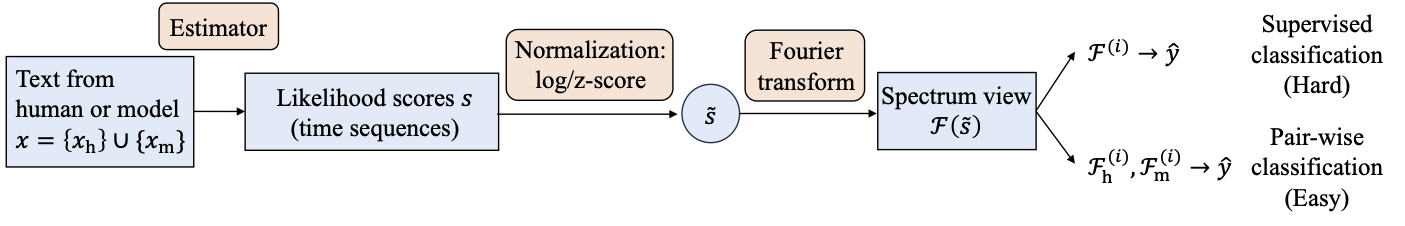
\includegraphics[width=1.0\textwidth]{images/procedure.png}
\vspace{0.3cm}
\small{
\begin{itemize}
    \item \textbf{Augmented spectrum-based classifier} trained using frequency features derived from multiple circularized variants of the original likelihood sequence
    \item Process involves \textbf{circularization of the score sequence}, \textbf{Fourier transform} of each circularized version, and \textbf{averaging the resulting spectra} to form a robust feature representation
    \item Inspired by \textbf{circular convolution in signal processing}, this approach acts as a form of \textbf{data augmentation} to amplify weak periodicity and extract salient features for classification
\end{itemize}
}
 \end{frame}


\section{Zero-shot Detection Methods}

\begin{frame}{FourierGPT(Zero-shot) Framework}
\centering
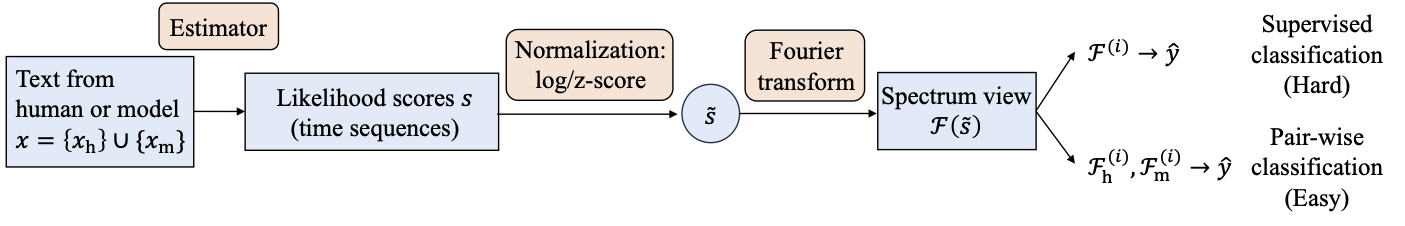
\includegraphics[width=1.0\textwidth]{images/procedure.png}
\vspace{0.3cm}
\small{
\begin{itemize}
    \item \textbf{Heuristic spectrum-based classifier} designed to distinguish human-written and machine-generated texts using \textbf{frequency-domain features}
    \item Classification decision based on summed spectral power difference over selected low-frequency range with an empirical threshold
    \[\left| \sum_{k=1}^{\delta} \| X_{\text{Human}}(\omega_k) \| - \sum_{k=1}^{\delta} \| X_{\text{Model}}(\omega_k) \| \right| > \varepsilon\]


\end{itemize}
}
\end{frame}

\section{Data Preprocessing}
\begin{frame}{Data Preprocessing for Supervised Method}
\textbf{English Data:}
\begin{itemize}
  \item Source:  {\footnotesize Ghostbuster dataset (https://github.com/vivek3141/ghostbuster-data)}
  \item Domains: \textbf{essay, reuter, wp}
  \item Each domain contains 6 types of LLM-generated texts and one human-written (HM) type
  \item \textbf{CSV with fields} — text, label {\footnotesize \textbf{(1 for LLM, 0 for HM)}}, domain
  \item Created mixed-domain and domain-specific CSV files
  \item Split into train, validation, test sets with ratio \textbf{8:1:1}
  \item Data cleaning applied to handle corrupted or missing entries
\end{itemize}

\textbf{Chinese Data:}
\begin{itemize}
  \item Domains: \textbf{news, webnovel, wiki}
  \item Human-written data and Qwen2-72b generated data
  \item \textbf{Same preprocessing pipeline} as English data
  \item Input format well structured; tested both \textbf{concatenated input-output} and \textbf{input only}
  \item Found better results \textbf{without concatenation} of input 
\end{itemize}
\end{frame}

\begin{frame}{Data Preprocessing for Zero-shot Method}
\begin{itemize}
  \item \textbf{Same datasets} as supervised method used for consistency
  \item For each domain, data split into \textbf{two separate text files}: one for human-written (HM), one for LLM-generated (LLM) texts
  \item Each line in txts corresponds to \textbf{one data entry} from the original dataset
  \item Related metadata such as topics and prompts stored in separate files, \textbf{aligned by line number} across HM and LLM files
  \item Missing or anomalous values identified and cleaned 
  \item For English data, each domain contains 6 LLM samples and 1 HM sample per topic, duplicate HM for 6 times to \textbf{balance sample counts}
\end{itemize}
\end{frame}


\begin{frame}{Processed Data Overview}
\begin{columns}[t]

\column{0.48\textwidth}
\textbf{CSV Files:}
\begin{itemize}
  \item \textbf{English Data:}
  \begin{itemize}
    \item eng\_essay.csv, eng\_reuter.csv, eng\_wp.csv
    \item eng\_hm\_essay.csv, eng\_hm\_reuter.csv, eng\_hm\_wp.csv
    \item eng\_llm\_essay.csv, eng\_llm\_reuter.csv, eng\_llm\_wp.csv
    \item eng\_mix (mixed domain)
  \end{itemize}
  \item \textbf{Chinese Data:}
  \begin{itemize}
    \item zh\_domain
    \item zh\_mix (mixed domain)
  \end{itemize}
\end{itemize}

\column{0.48\textwidth}
\textbf{TXT Files:}
\begin{itemize}
  \item \textbf{English Data:}
  \begin{itemize}
    \item eng\_essay\_hm.txt, eng\_essay\_llm.txt
    \item eng\_reuter\_hm.txt, eng\_reuter\_llm.txt
    \item eng\_wp\_hm.txt, eng\_wp\_llm.txt
  \end{itemize}
  \item \textbf{Chinese Data:(similar)}
  \begin{itemize}
    \item zh\_news\_hm.txt, zh\_news\_llm.txt
    \item zh\_webnovel\_hm.txt, zh\_webnovel\_llm.txt
    \item zh\_wiki\_hm.txt, zh\_wiki\_llm.txt
  \end{itemize}
\end{itemize}

\end{columns}
\end{frame}



\section{Experiment Design}

\begin{frame}{Supervised Learning Method Experiment}
\begin{itemize}
  \item Training parameters:
  \begin{itemize}
    \item Epochs: 10
    \item Learning rate Eng: \(1 \times 10^{-7}\), Zh: \(1 \times 10^{-5}\)
    \item Batch size: 16
    \item Log interval: 50 steps
    \item Optimizer: AdamW
  \end{itemize}
  \item Models used:
  \begin{itemize}
    \item English: bert-base-uncased, bert-base-multilingual-cased, roberta-base, xlm-roberta-base
    \item Chinese: bert-base-chinese, xlm-roberta-base, roberta-base
  \end{itemize}
  \item \textbf{Controlled variables} to ensure fair comparison:
  \begin{itemize}
    \item Same training and validation splits used across all models
    \item Consistent batch size, number of epochs, and optimizer settings per language
    \item Evaluation metrics include accuracy, precision, recall, F1, and AUROC
  \end{itemize}
  \item \textbf{Final step: Compare the five evaluation metrics across models and datasets}
\end{itemize}
\end{frame}

\begin{frame}{Supervised Learning Method: Experimental Setup}
\begin{itemize}
  \item \textbf{In-Domain Evaluation:}
  \begin{itemize}
    \item \textbf{Combine} data from all three domains (essay, reuter, wp) and \textbf{shuffle}
    \item Split into train, validation, and test sets with ratio 8:1:1
    \item Compute five evaluation metrics (accuracy, precision, recall, F1, AUROC) on test set
    \item Report both \textbf{overall metrics} and metrics for \textbf{each individual domain}
  \end{itemize}
  \item \textbf{Out-of-Domain (OOD) Evaluation:}
  \begin{itemize}
    \item For each domain (A, B, C), \textbf{train and validate} \textbf{only} on data from \textbf{domain A}
    \item Use \textbf{mixed-domain} data as the \textbf{test} set
    \item Compute the five metrics on the test set overall and for each domain within test
    \item \textbf{Discard metrics for domain A} in test, since training and validation data overlap
    \item Repeat the same procedure by training/validating on domain B and C, respectively
  \end{itemize}
\end{itemize}
\end{frame}

\begin{frame}{FourierGPT supervised learning experiment}
\begin{itemize}
  \item Models used:
  \begin{itemize}
    \item English: gpt2-xl, Mistral-7B-v0.1
    \item Chinese: gpt2-chinese-cluecorpussmall, Wenzhong2.0-GPT2-3.5B-chinese
  \end{itemize}
\item \textbf{Controlled variables} to ensure fair comparison:
  \begin{itemize}
    \item Consistent spectrum generation using circular shifts on NLL data with\textbf{ fixed interpolation length}
    \item Standard scaling, \textbf{fixed feature selection ($k=120$)}, and \textbf{SVM} with \textbf{RBF kernel} and fixed hyperparameters
    \item Comprehensive evaluation metrics including accuracy, precision, recall, F1 score, and AUROC; 
  \end{itemize}
\end{itemize}
\end{frame}

\begin{frame}{Zero-shot detection method experiment}
\begin{itemize}
  \item Models used:
  \begin{itemize}
    \item English: gpt2-xl, Mistral-7B-v0.1
    \item Chinese: gpt2-chinese-cluecorpussmall, Wenzhong2.0-GPT2-3.5B-chinese
  \end{itemize}
  \item \textbf{Controlled variables} to ensure fair comparison:
  \begin{itemize}
    \item Same procedure to generate spectrum across all models
    \item Same k range and threshold $\epsilon = 0$
    \item Evaluation metrics include accuracy, and plot AUROC curve 
  \end{itemize}
\end{itemize}
\end{frame}

\begin{frame}{Zero-shot Detection Method: Experimental Setup}
\begin{itemize}
  \item A sample is classified as model-generated if
 \textbf{ \( \sum_{i=1}^k P_{\text{model}}(\omega_i) - \sum_{i=1}^k P_{\text{human}}(\omega_i) > \varepsilon \)}; otherwise, it is classified as human-written.
  \item The optimal \( k \in [1, 50] \) is selected by evaluating accuracy, precision, recall, and F1 score for each \( k \), and choosing the one with the \textbf{highest accuracy}.
  \item Given the \textbf{selected \( k \)}, multiple power thresholds are tested to compute true positive rate (TPR) and false positive rate (FPR) pairs, forming the ROC curve and enabling the calculation of AUROC.

\end{itemize}
\end{frame}


%------------------------------------
\section{Result}
\begin{frame}{Supervised Learning Method(Eng):in domain}
\centering
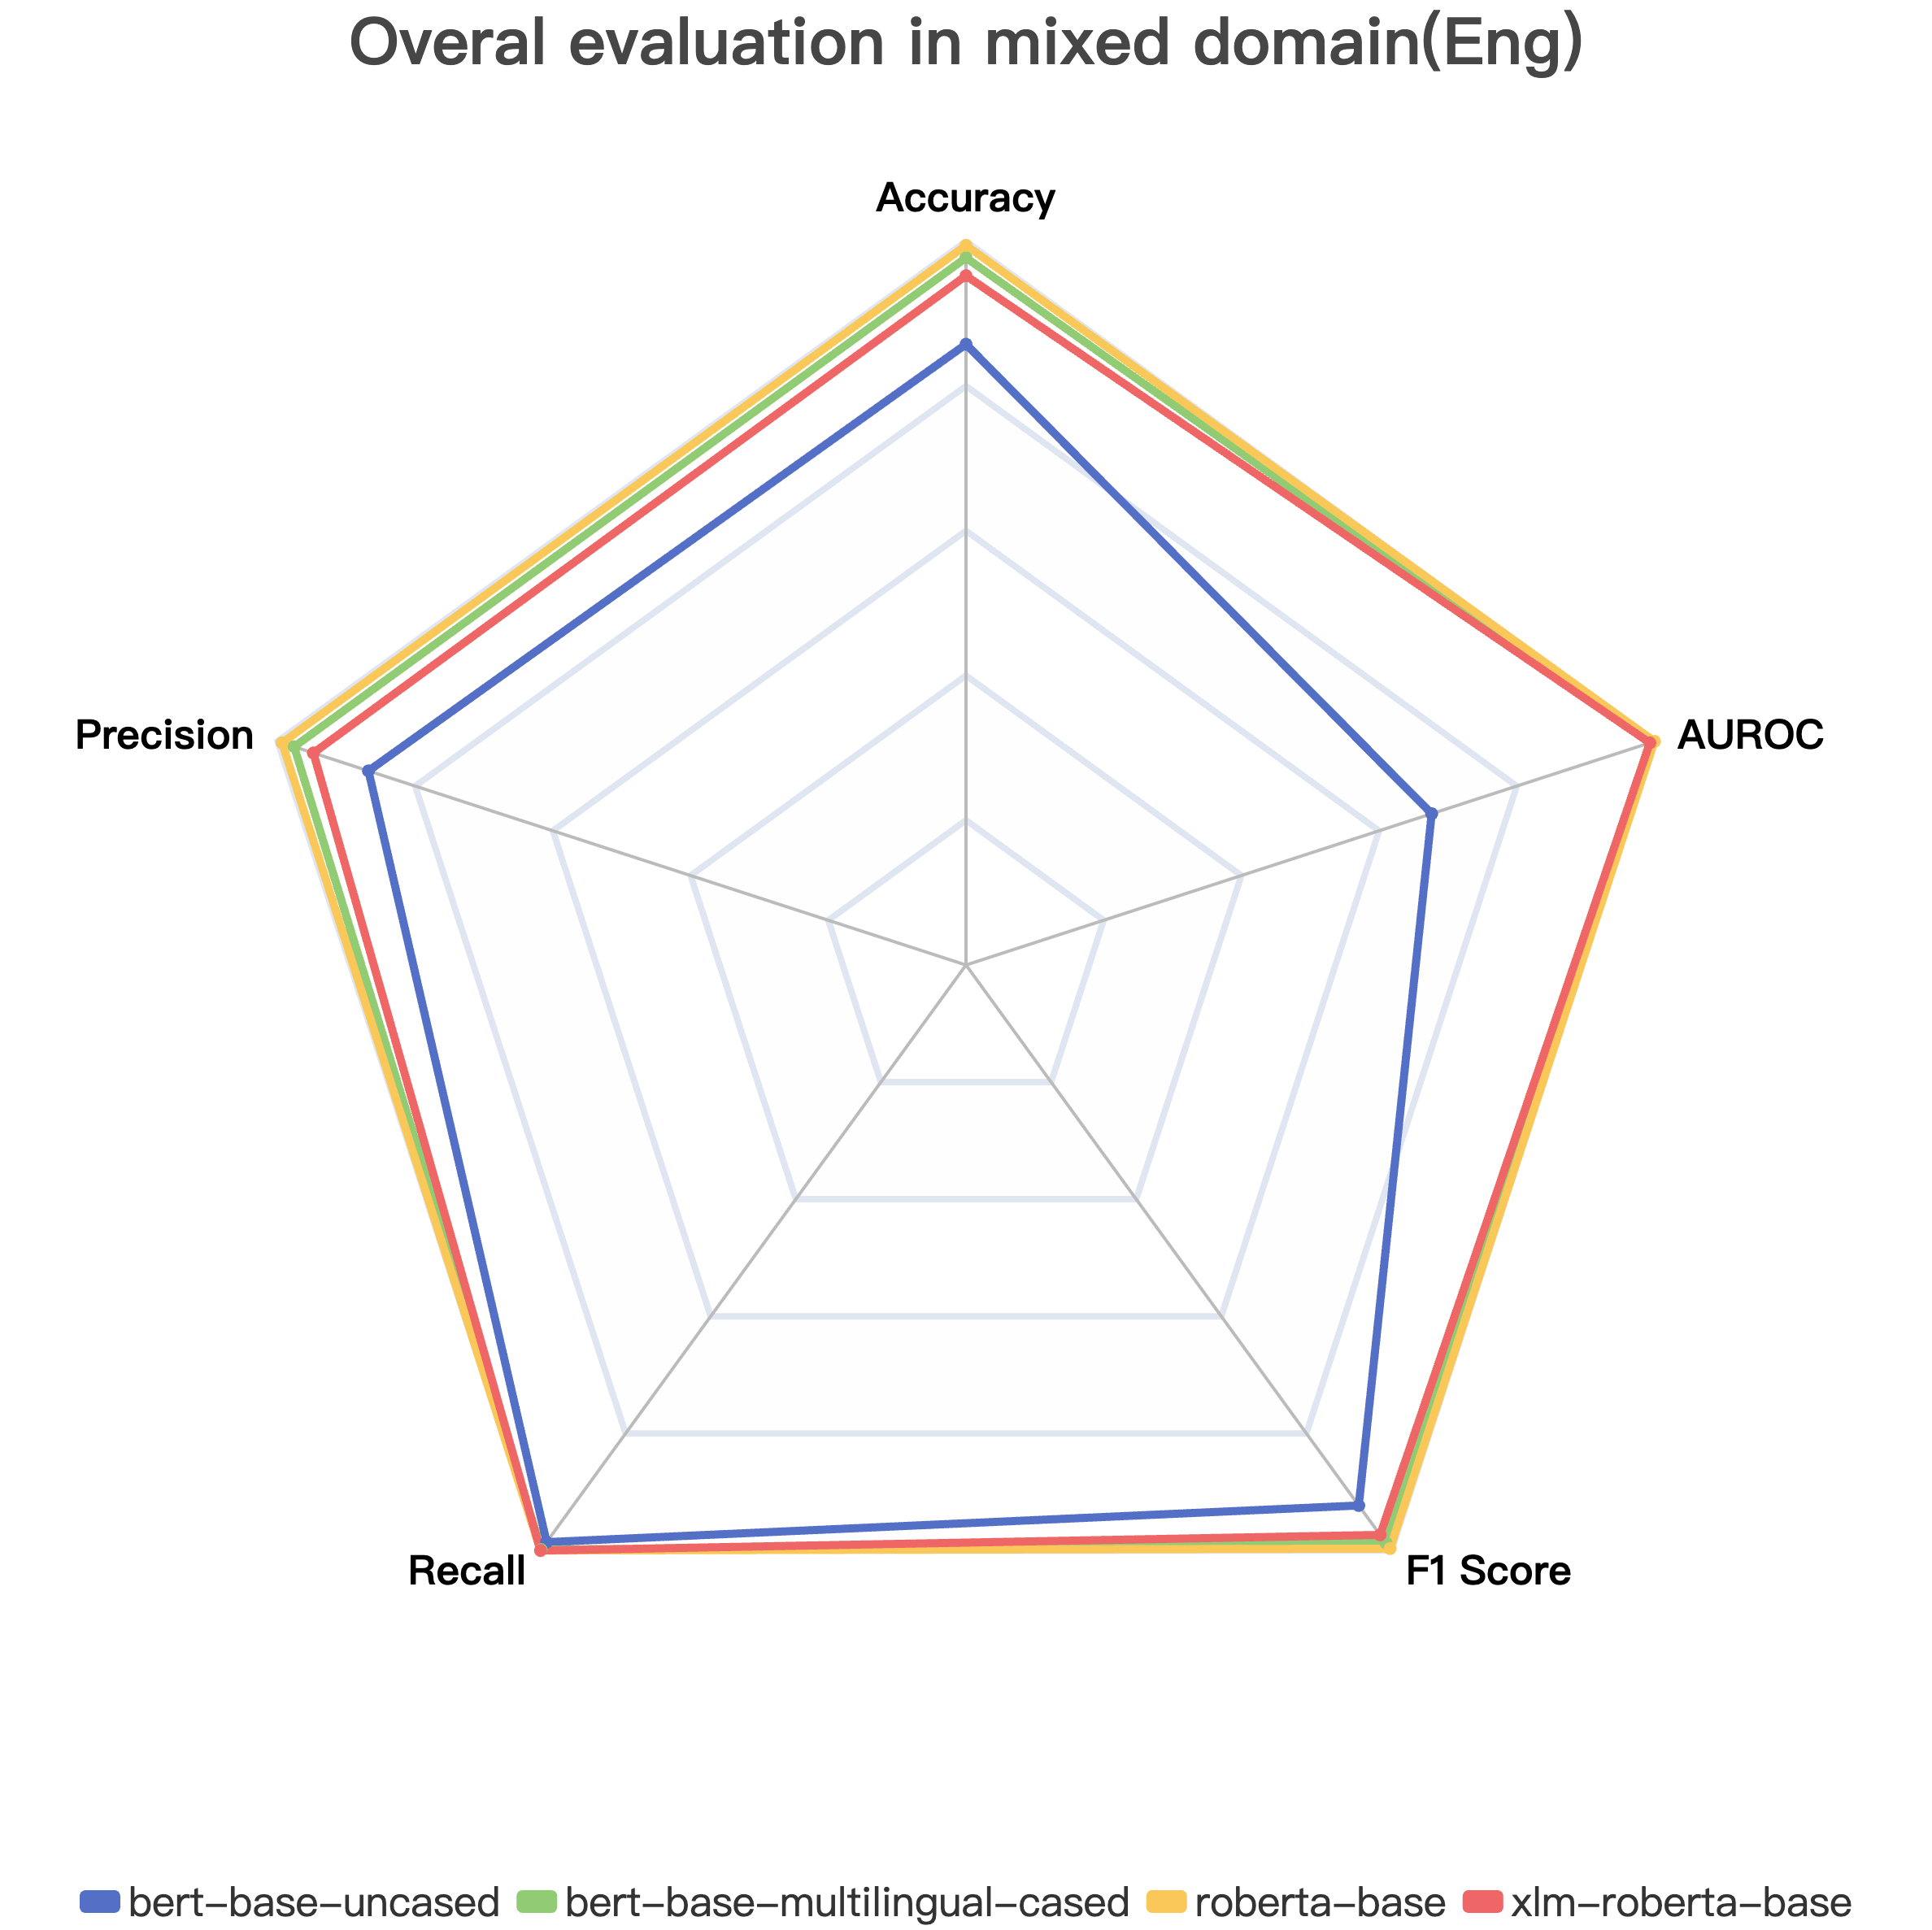
\includegraphics[width=0.6\textwidth]{images/Overal evaluation in mixed domain(Eng).png}

\begin{flushleft}
\scriptsize
In the English mixed domain, \textbf{roberta-base and xlm-roberta-base} outperform bert-base-uncased and bert-base-multilingual-cased in accuracy, F1 score, and AUROC.
\normalize
\end{flushleft}
\end{frame}

\begin{frame}{Supervised Learning Method (Eng): Out of Domain}
\begin{columns}[t]
  \column{0.35\textwidth}
    \centering
    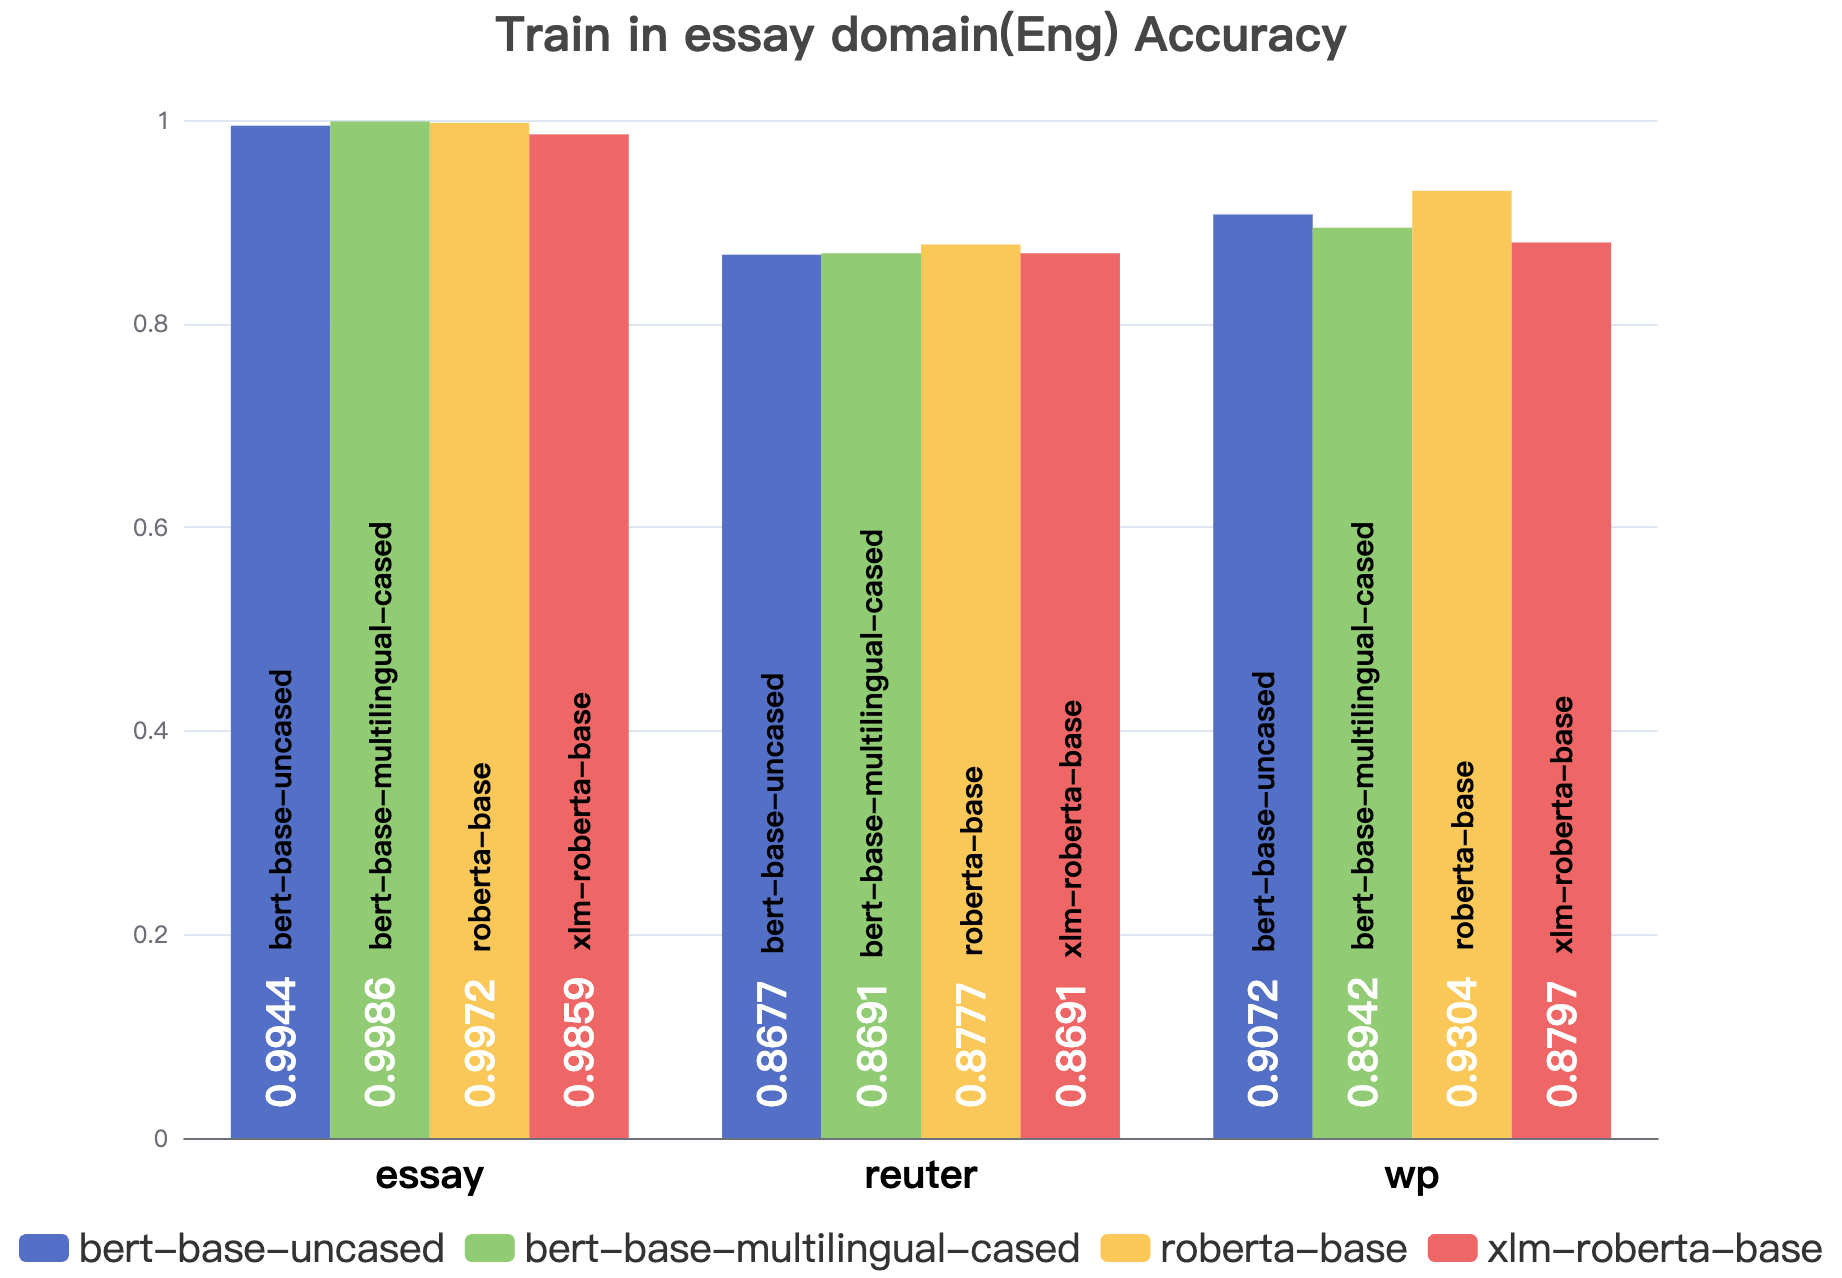
\includegraphics[width=\linewidth]{images/Train in essay domain(Eng) Accuracy.png}



  \column{0.35\textwidth}
    \centering
    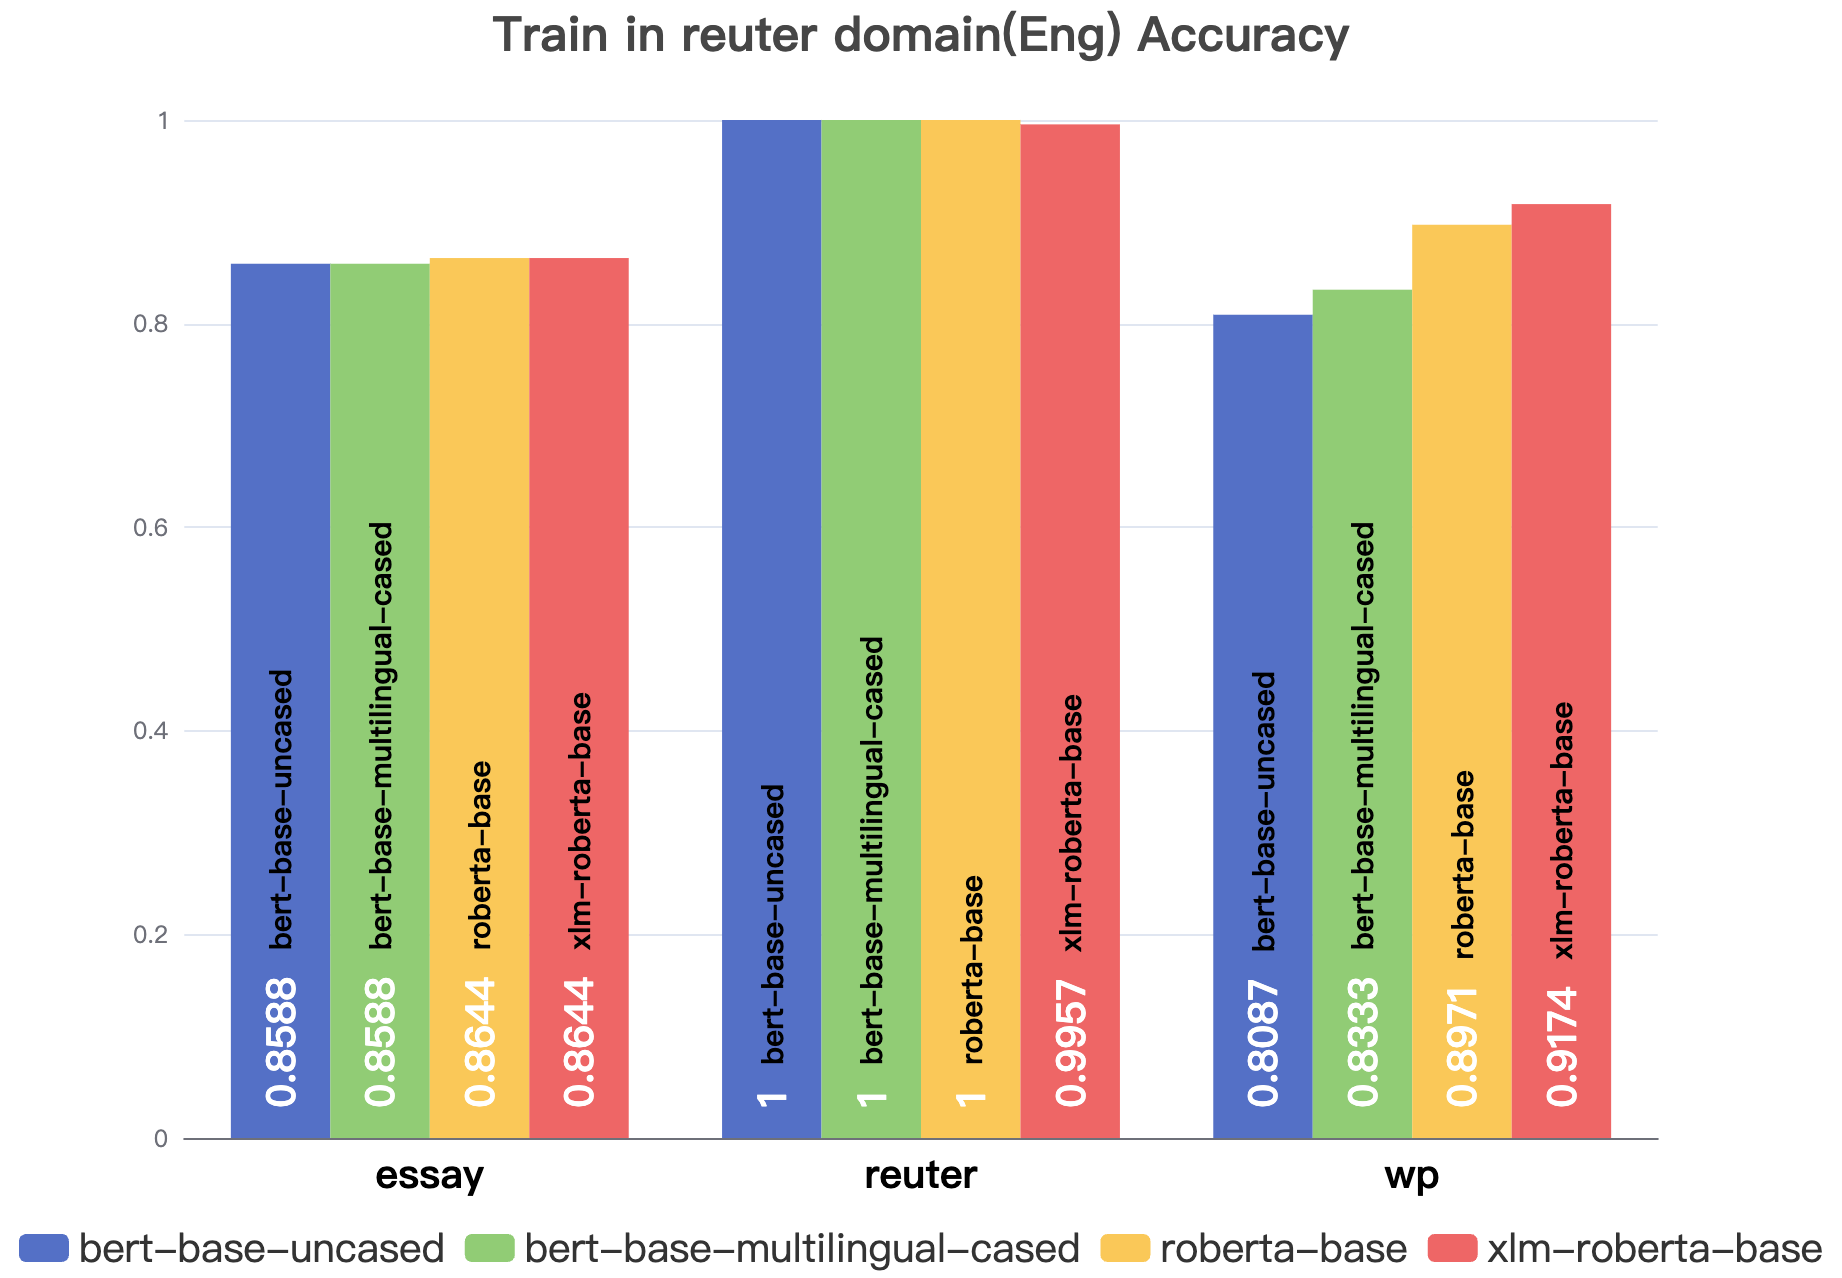
\includegraphics[width=\linewidth]{images/Train in reuter domain(Eng) Accuracy.png}



  \column{0.35\textwidth}
    \centering
    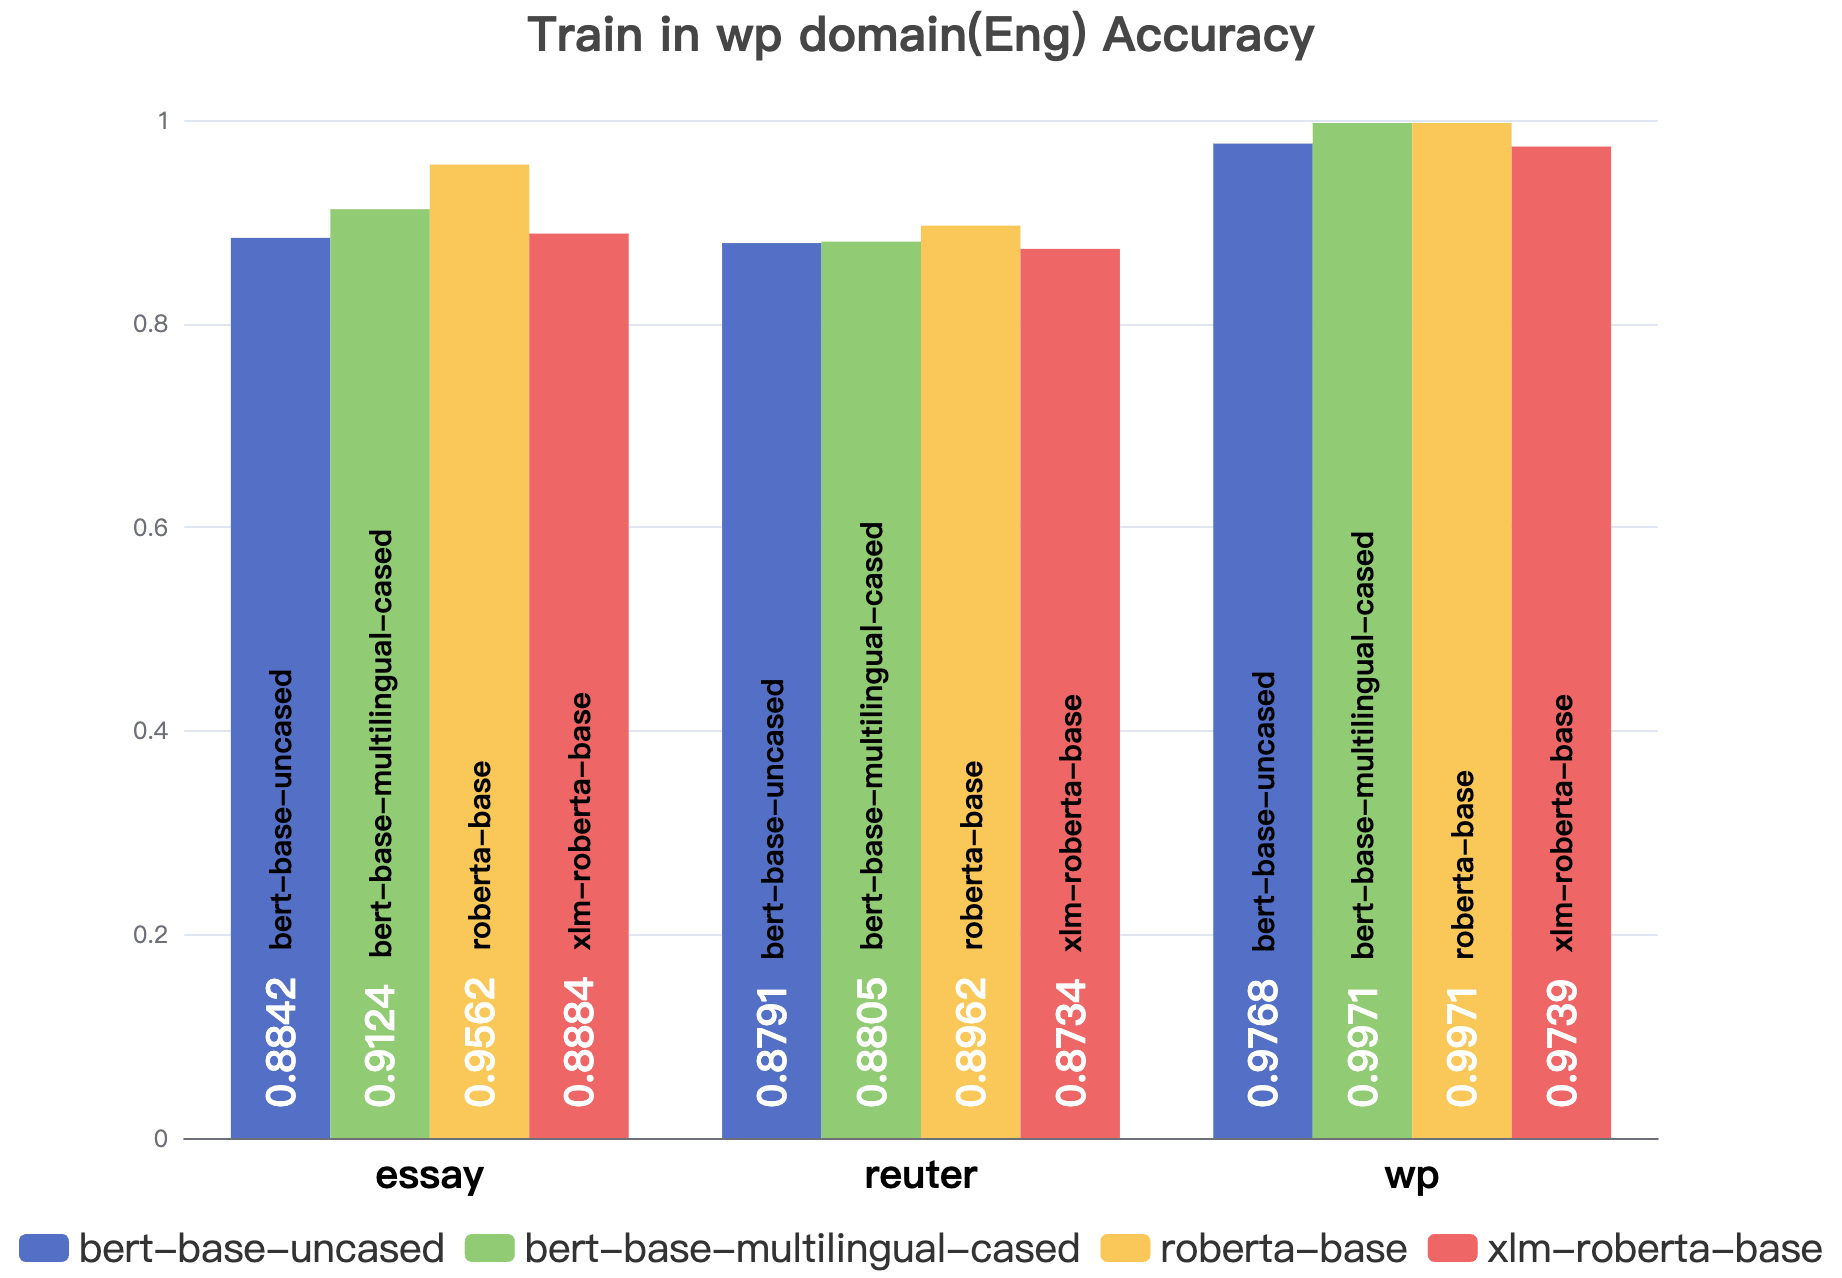
\includegraphics[width=\linewidth]{images/Train in wp domain(Eng) Accuracy.png}
\end{columns}

\begin{itemize}
    \item Perform well within their \textbf{own training domain}, achieving accuracy generally \textbf{above 0.88}
    \item Accuracy significantly decreases when \textbf{tested on other domains}, often dropping \textbf{below 0.80}
    \item Among the four models, \textbf{roberta-base} shows relatively better generalization across different domains.
    
\end{itemize}

\end{frame}
%----------------------------------------

\begin{frame}{Supervised Learning Method: Loss Curve (Eng)}
\begin{figure}[htbp]
    \centering
    \begin{subfigure}[b]{0.44\linewidth}
        \centering
        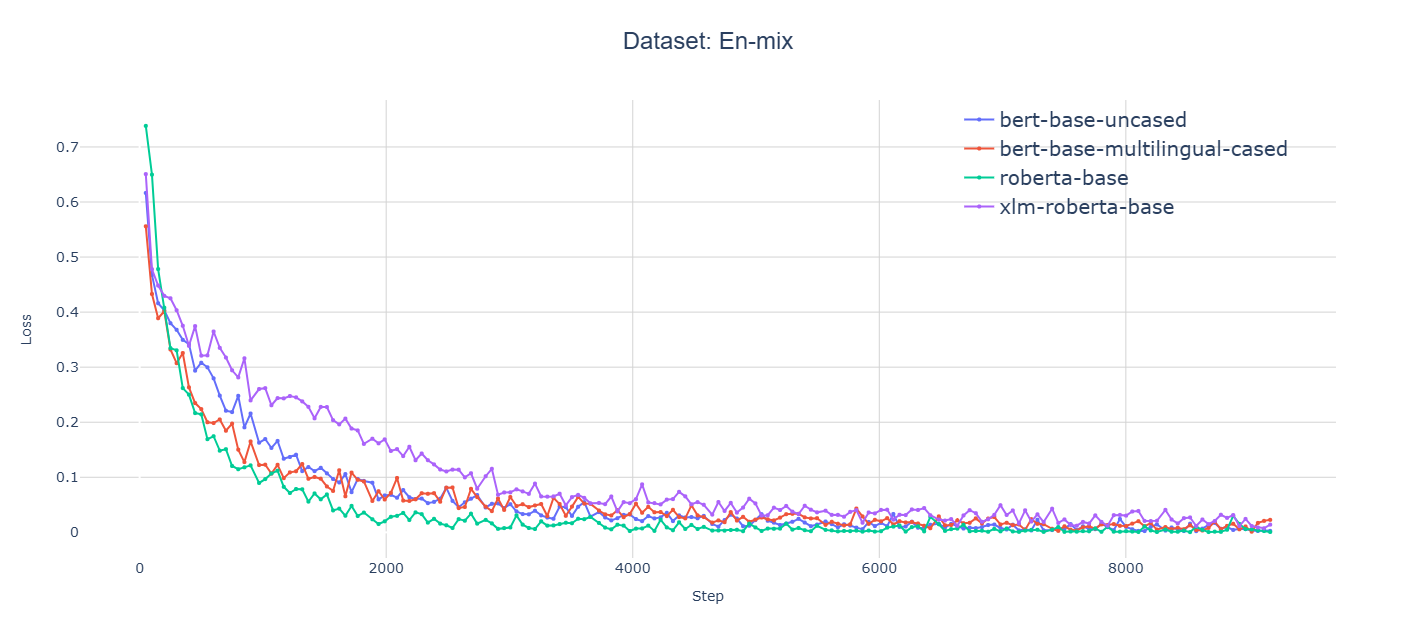
\includegraphics[width=\linewidth]{images/en_mix.png}
        \caption{Eng-mix}
        \label{fig:en-mix}
    \end{subfigure}
    \hfill
    \begin{subfigure}[b]{0.44\linewidth}
        \centering
        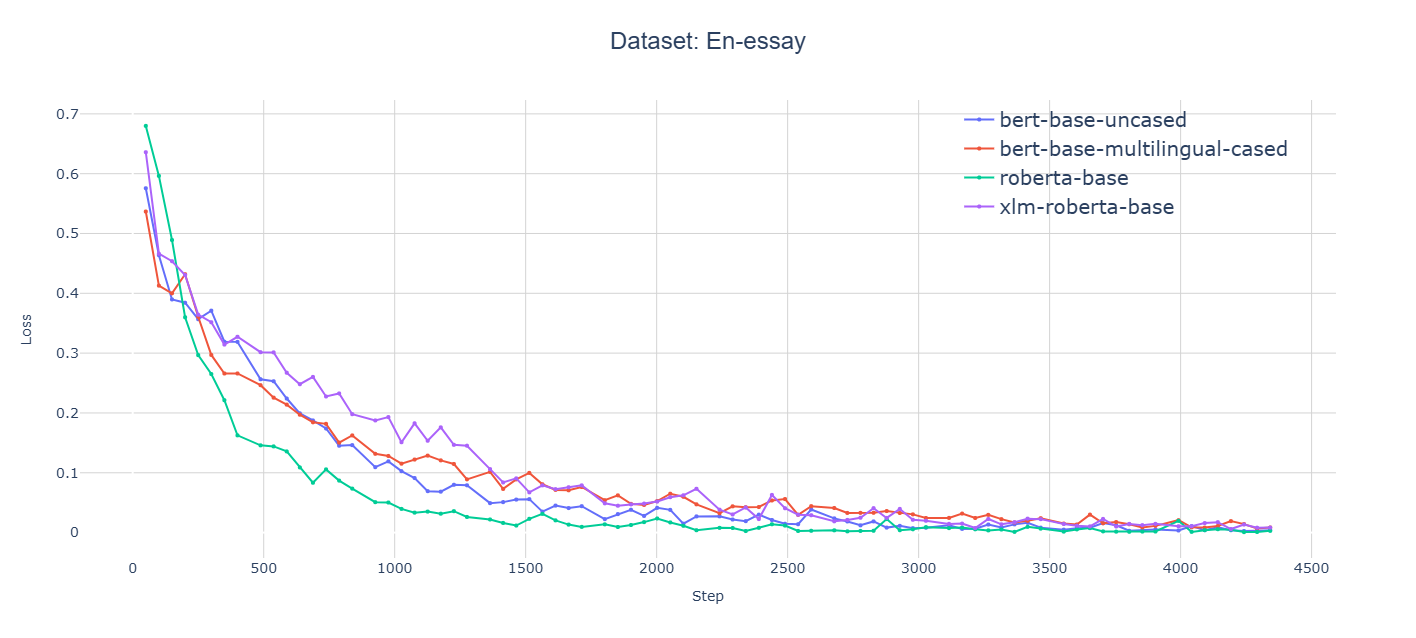
\includegraphics[width=\linewidth]{images/en_essay.png}
        \caption{Eng-essay}
        \label{fig:en-essay}
    \end{subfigure}

    \vspace{-0.2em}  % 控制两行子图之间的垂直间距

    \begin{subfigure}[b]{0.44\linewidth}
        \centering
        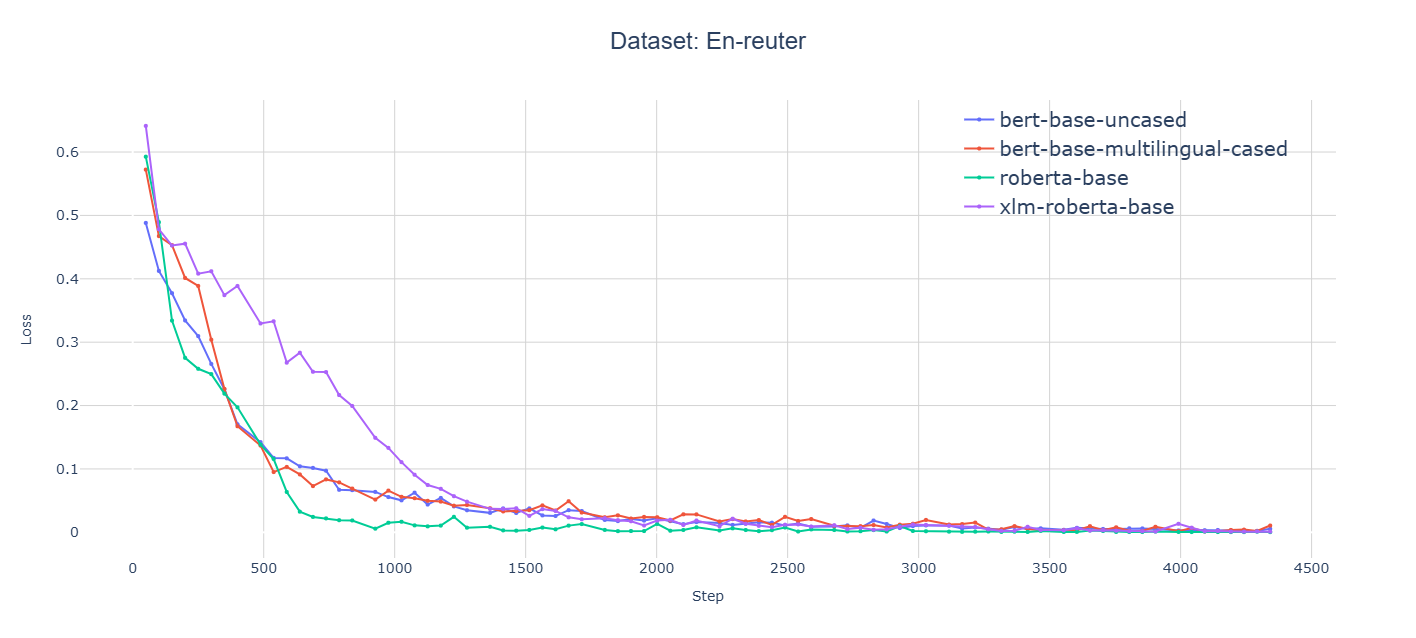
\includegraphics[width=\linewidth]{images/en_reuter.png}
        \caption{Eng-reuter}
        \label{fig:en-reuter}
    \end{subfigure}
    \hfill
    \begin{subfigure}[b]{0.44\linewidth}
        \centering
        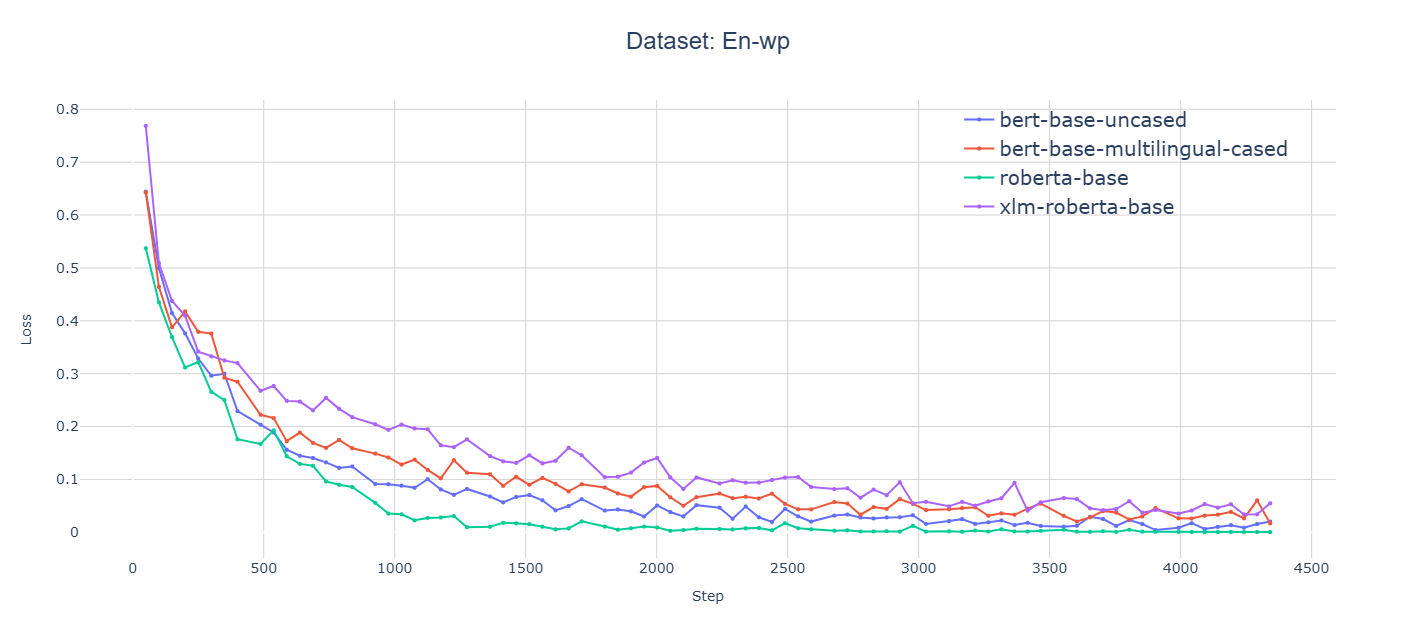
\includegraphics[width=\linewidth]{images/en_wp.png}
        \caption{Eng-wp}
        \label{fig:en-wp}
    \end{subfigure}

    \label{fig:four-plots}
    \vspace{-1em}  % 在图下方空出几行以写正文
\end{figure}
\footnotesize
Among the four models, \textbf{roberta-base} exhibits the fastest loss decline across all datasets. Eventually, all models \textbf{converge and stabilize} with the loss values near \textbf{0.005 to 0.001}, indicating effective training and good convergence behavior.

\end{frame}

%------------------------------
\begin{frame}{Supervised Learning Method: Metrics Comparison (Eng)}

\centering
\tiny
\setlength{\tabcolsep}{2pt}
\renewcommand{\arraystretch}{1.0}

\resizebox{0.95\textwidth}{!}{%
\begin{tabular}{|l|c|c|c|c|}
\hline
\textbf{FT domain} & \textbf{mixed} & \textbf{essay} & \textbf{reuter} & \textbf{wp} \\
\hline
Accuracy & 
0.8577 / 0.8460 / 0.8578 / 0.8696 & 
0.9234 / 0.9944 / 0.8677 / 0.9072 & 
0.8896 / 0.8588 / 1.0000 / 0.8087 & 
0.9129 / 0.8842 / 0.8791 / 0.9768 \\
\hline
Precision & 
0.8679 / 0.8640 / 0.8590 / 0.8813 & 
0.9291 / 0.9935 / 0.8889 / 0.9091 & 
0.9421 / 0.8657 / 1.0000 / 0.9797 & 
0.9107 / 0.8829 / 0.8811 / 0.9742 \\
\hline
Recall & 
0.9857 / 0.9755 / 0.9983 / 0.9834 & 
0.9868 / 1.0000 / 0.9669 / 0.9934 & 
0.9297 / 0.9902 / 1.0000 / 0.7980 & 
0.9973 / 0.9984 / 0.9934 / 1.0000 \\
\hline
F1 Score & 
0.9231 / 0.9163 / 0.9234 / 0.9296 & 
0.9571 / 0.9967 / 0.9262 / 0.9494 & 
0.9358 / 0.9238 / 1.0000 / 0.8796 & 
0.9520 / 0.9371 / 0.9339 / 0.9869 \\
\hline
AUROC & 
0.6764 / 0.6967 / 0.5726 / 0.8464 & 
0.9526 / 0.9999 / 0.9178 / 0.9474 & 
0.8558 / 0.8016 / 1.0000 / 0.9022 & 
0.9435 / 0.8843 / 0.8828 / 1.0000 \\
\hline
\end{tabular}%
}

\vspace{0.1cm}
{\scriptsize \captionof{table}{bert-base-uncased (Eng) overall/essay/reuter/wp}}

\vspace{0.3cm}

\resizebox{0.95\textwidth}{!}{%
\begin{tabular}{|l|c|c|c|c|}
\hline
\textbf{FT domain} & \textbf{mixed} & \textbf{essay} & \textbf{reuter} & \textbf{wp} \\
\hline
Accuracy & 
0.9772 / 0.9774 / 0.9844 / 0.9696 & 
0.9210 / 0.9986 / 0.8691 / 0.8942 & 
0.8977 / 0.8588 / 1.0000 / 0.8333 & 
0.9296 / 0.9124 / 0.8805 / 0.9971 \\
\hline
Precision & 
0.9758 / 0.9760 / 0.9837 / 0.9679 & 
0.9432 / 0.9984 / 0.9051 / 0.9275 & 
0.9412 / 0.8636 / 1.0000 / 0.9785 & 
0.9553 / 0.9270 / 0.9437 / 0.9967 \\
\hline
Recall & 
0.9984 / 0.9984 / 0.9983 / 0.9983 & 
0.9670 / 1.0000 / 0.9470 / 0.9536 & 
0.9407 / 0.9935 / 1.0000 / 0.8278 & 
0.9637 / 0.9755 / 0.9156 / 1.0000 \\
\hline
F1 Score & 
0.9870 / 0.9871 / 0.9910 / 0.9829 & 
0.9550 / 0.9992 / 0.9256 / 0.9404 & 
0.9409 / 0.9240 / 1.0000 / 0.8969 & 
0.9595 / 0.9506 / 0.9294 / 0.9983 \\
\hline
AUROC & 
0.9938 / 0.9942 / 0.9948 / 0.9948 & 
0.8951 / 1.0000 / 0.8050 / 0.8857 & 
0.8161 / 0.6701 / 1.0000 / 0.9163 & 
0.9573 / 0.8957 / 0.9276 / 0.9999 \\
\hline
\end{tabular}
}

\vspace{0.1cm}
{\scriptsize \captionof{table}{bert-base-multilingual (Eng) overall/essay/reuter/wp}}
\end{frame}





\begin{frame}{Supervised Learning Method: Metrics Comparison (Eng)}

\centering
\tiny
\setlength{\tabcolsep}{2pt}
\renewcommand{\arraystretch}{1.0}

% roberta-base
\resizebox{0.95\textwidth}{!}{%
\begin{tabular}{|l|c|c|c|c|}
\hline
\textbf{FT domain} & \textbf{mixed} & \textbf{essay} & \textbf{reuter} & \textbf{wp} \\
\hline
Accuracy & 
0.9943 / 0.9887 / 0.9972 / 0.9971 & 
0.9353 / 0.9972 / 0.8777 / 0.9304 & 
0.9205 / 0.8644 / 1.0000 / 0.8971 & 
0.9495 / 0.9562 / 0.8962 / 0.9971 \\
\hline
Precision & 
0.9934 / 0.9871 / 0.9967 / 0.9967 & 
0.9340 / 0.9967 / 0.8787 / 0.9330 & 
0.9160 / 0.8644 / 1.0000 / 0.8948 & 
0.9482 / 0.9532 / 0.8992 / 0.9967 \\
\hline
Recall & 
1.0000 / 1.0000 / 1.0000 / 1.0000 & 
0.9956 / 1.0000 / 0.9950 / 0.9917 & 
1.0000 / 1.0000 / 1.0000 / 1.0000 & 
0.9962 / 0.9984 / 0.9901 / 1.0000 \\
\hline
F1 Score & 
0.9967 / 0.9935 / 0.9983 / 0.9983 & 
0.9638 / 0.9984 / 0.9332 / 0.9615 & 
0.9561 / 0.9273 / 1.0000 / 0.9445 & 
0.9716 / 0.9753 / 0.9425 / 0.9983 \\
\hline
AUROC & 
1.0000 / 1.0000 / 1.0000 / 1.0000 & 
0.9797 / 1.0000 / 0.9662 / 0.9696 & 
0.9024 / 0.9039 / 1.0000 / 0.9316 & 
0.9826 / 0.9799 / 0.9392 / 1.0000 \\
\hline
\end{tabular}%
}

\vspace{0.1cm}
{\scriptsize \captionof{table}{roberta-base (Eng) overall/essay/reuter/wp}}

\vspace{0.3cm}

% xlm-roberta-base
\resizebox{0.95\textwidth}{!}{%
\begin{tabular}{|l|c|c|c|c|}
\hline
\textbf{FT domain} & \textbf{mixed} & \textbf{essay} & \textbf{reuter} & \textbf{wp} \\
\hline
Accuracy & 
0.8777 / 0.8686 / 0.8649 / 0.9000 & 
0.9119 / 0.9859 / 0.8691 / 0.8797 & 
0.9257 / 0.8644 / 0.9957 / 0.9174 & 
0.9115 / 0.8884 / 0.8734 / 0.9739 \\
\hline
Precision & 
0.8766 / 0.8691 / 0.8641 / 0.8975 & 
0.9123 / 0.9839 / 0.8678 / 0.8917 & 
0.9249 / 0.8644 / 0.9951 / 0.9253 & 
0.9093 / 0.8913 / 0.8716 / 0.9711 \\
\hline
Recall & 
0.9995 / 0.9984 / 1.0000 / 1.0000 & 
0.9940 / 1.0000 / 1.0000 / 0.9818 & 
0.9951 / 1.0000 / 1.0000 / 0.9851 & 
0.9973 / 0.9918 / 1.0000 / 1.0000 \\
\hline
F1 Score & 
0.9340 / 0.9293 / 0.9271 / 0.9460 & 
0.9514 / 0.9919 / 0.9292 / 0.9346 & 
0.9587 / 0.9273 / 0.9975 / 0.9543 & 
0.9513 / 0.9389 / 0.9314 / 0.9853 \\
\hline
AUROC & 
0.9618 / 0.9502 / 0.9653 / 0.9800 & 
0.8359 / 0.9999 / 0.6537 / 0.7428 & 
0.8115 / 0.5012 / 1.0000 / 0.9369 & 
0.9291 / 0.8743 / 0.8691 / 0.9978 \\
\hline
\end{tabular}
}

\vspace{0.1cm}
{\scriptsize \captionof{table}{xlm-roberta-base (Eng) overall/essay/reuter/wp}}

\end{frame}






% ------------------------------------
\begin{frame}{Supervised Learning Method(Zh):in domain}

\centering
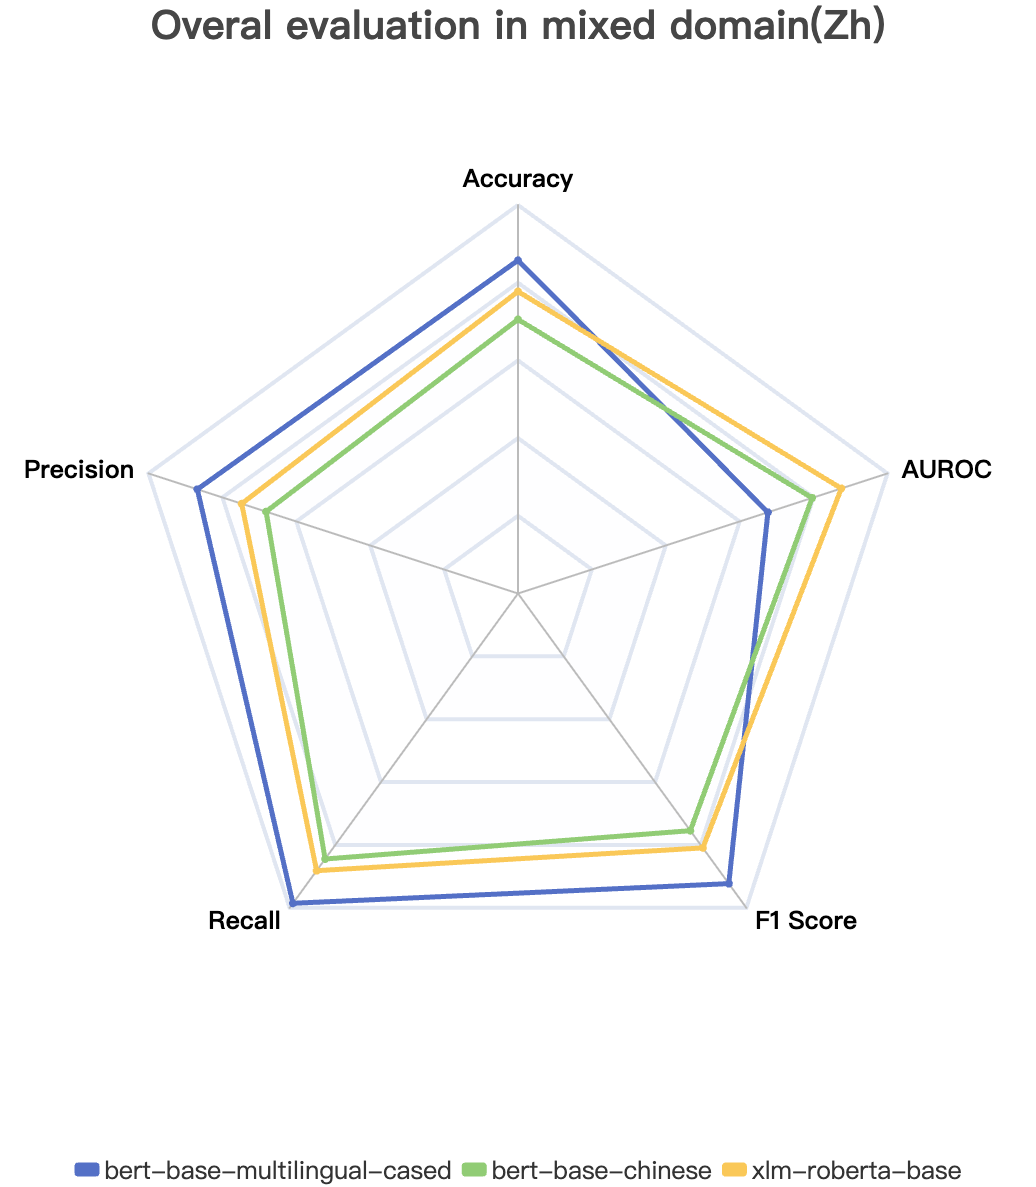
\includegraphics[width=0.5\textwidth]{images/Overal evaluation in mixed domain(Zh).png}

\vspace{-0.2em}
\begin{flushleft}
\scriptsize
In the Chinese mixed domain, \textbf{bert-base-multilingual-cased} achieves the highest recall and precision, while \textbf{xlm-roberta-base} leads in AUROC and F1 score, outperforming bert-base-chinese across most metrics.
\normalize
\end{flushleft}

\end{frame}


\begin{frame}{Supervised Learning Method (Zh): Out of Domain}
\begin{columns}[t]
  \column{0.35\textwidth}
    \centering
    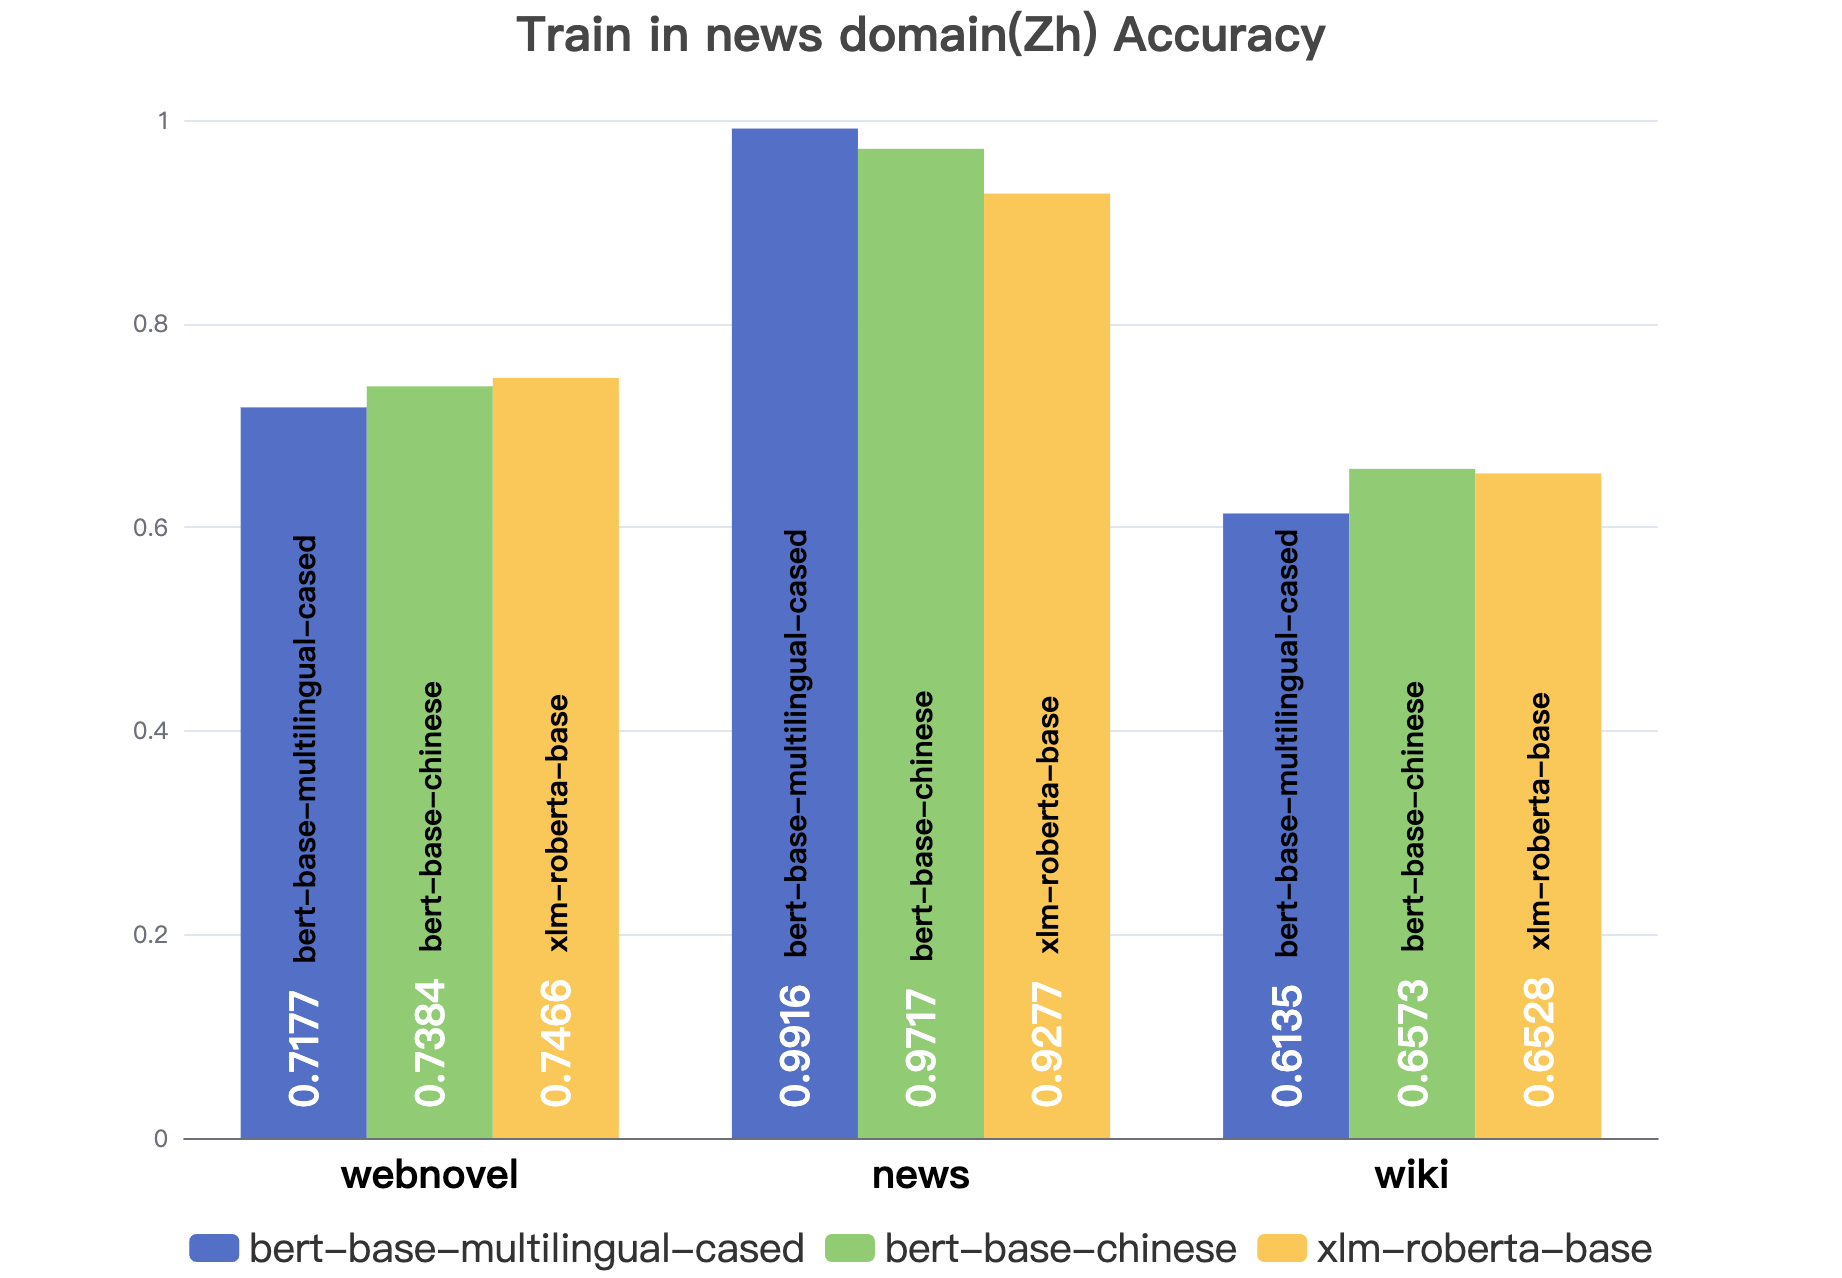
\includegraphics[width=\linewidth]{images/Train in news domain(Zh) Accuracy.png}

  \column{0.35\textwidth}
    \centering
    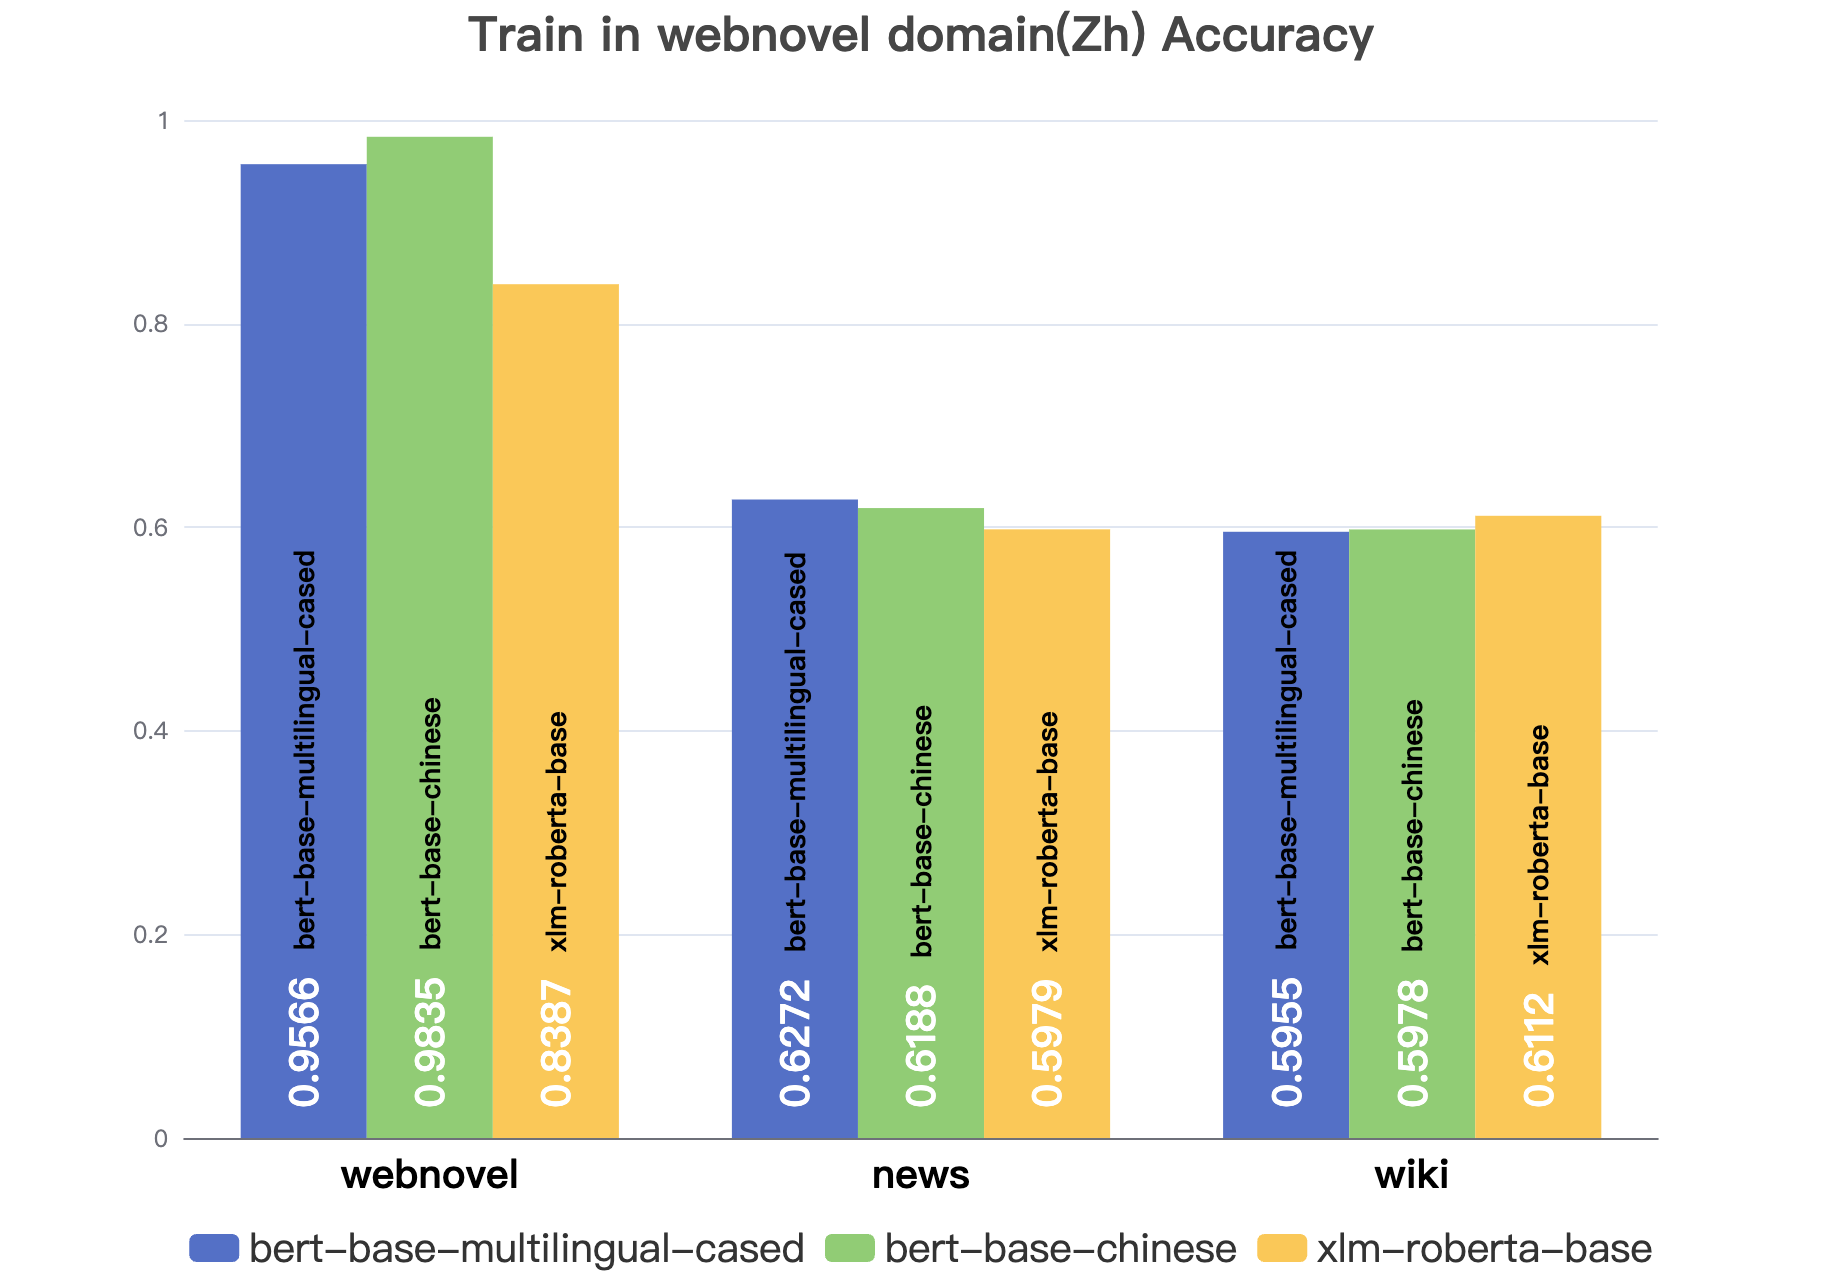
\includegraphics[width=\linewidth]{images/Train in webnovel domain(Zh) Accuracy.png}

  \column{0.35\textwidth}
    \centering
    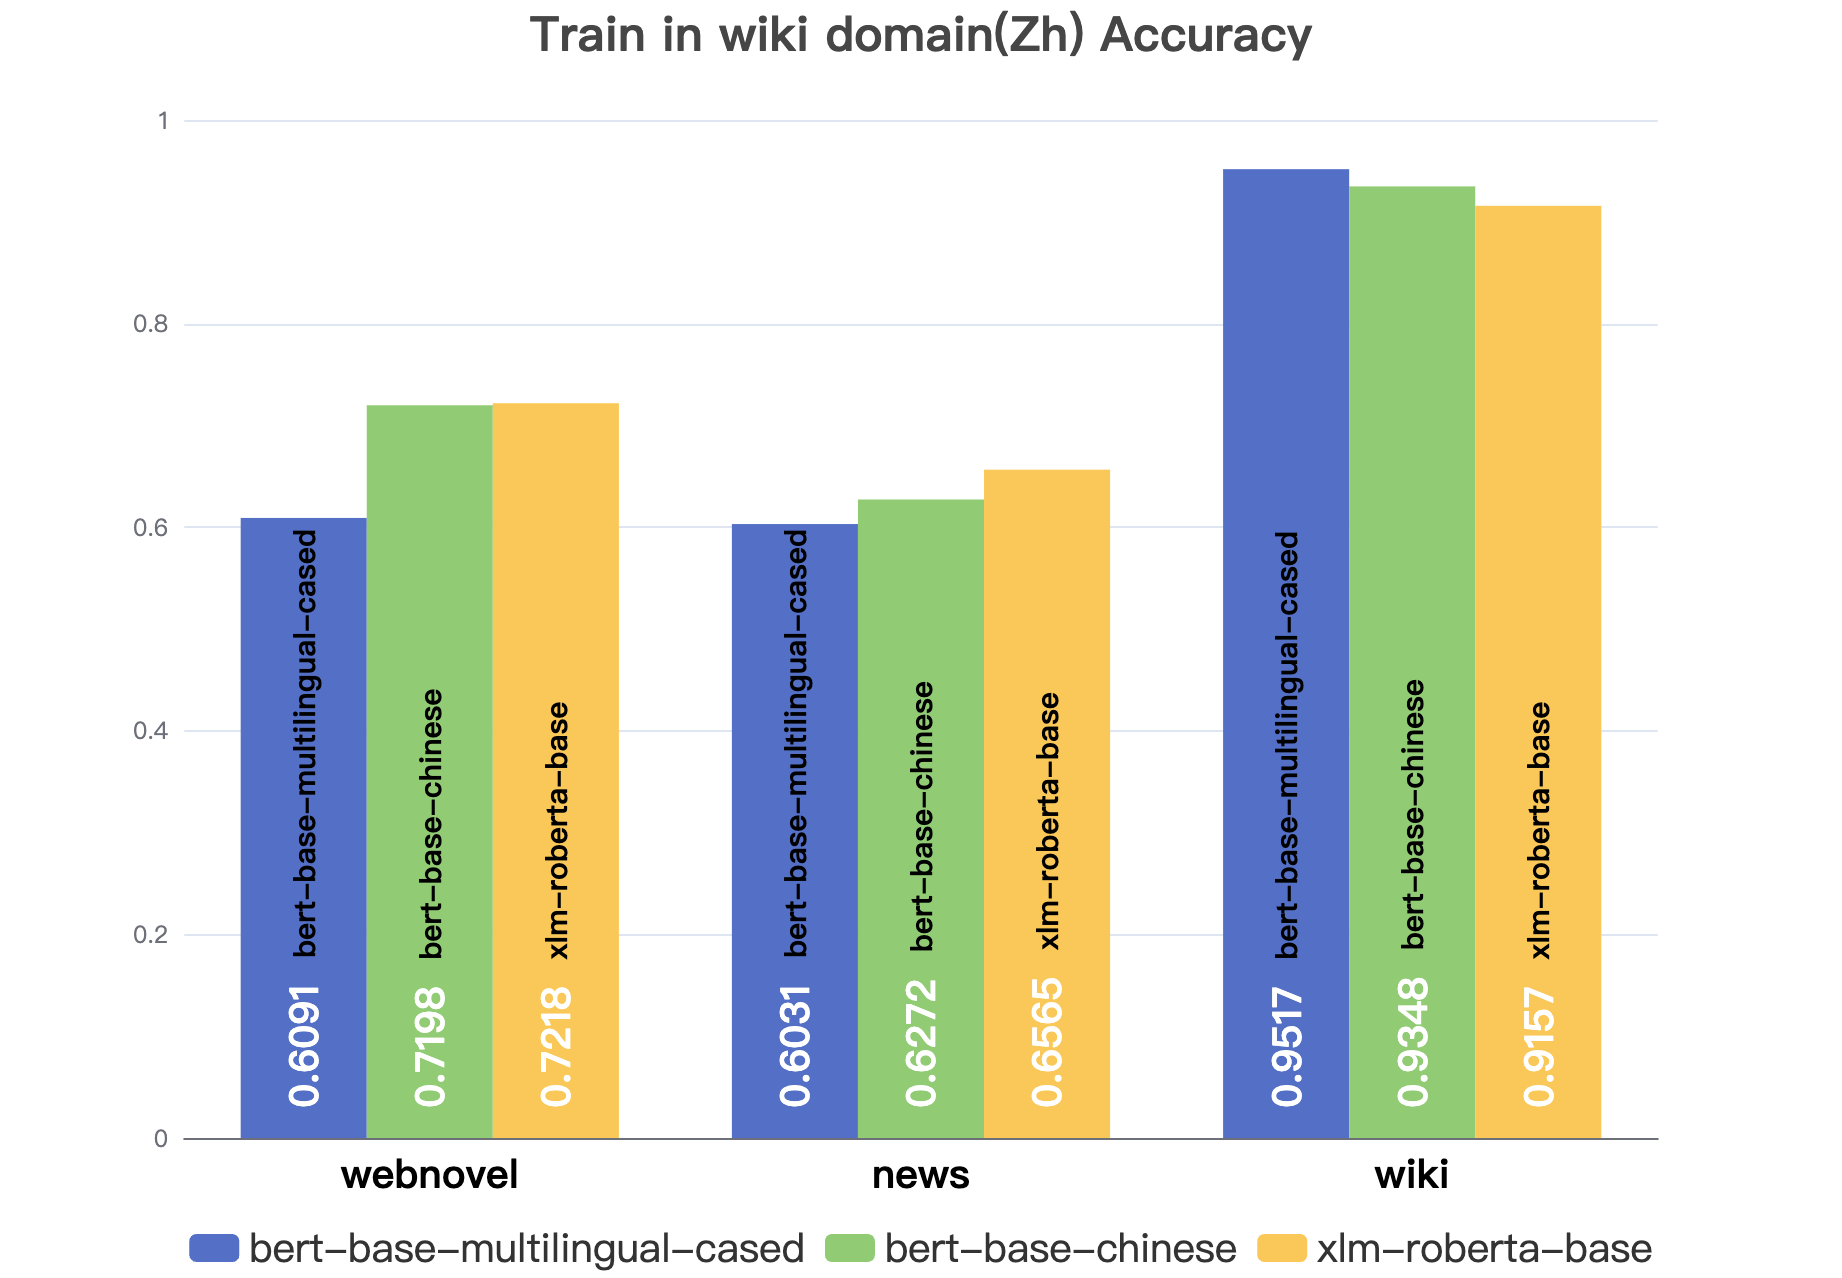
\includegraphics[width=\linewidth]{images/Train in wiki domain(Zh) Accuracy.png}
\end{columns}

\begin{itemize}
    \item Performance is strong within their \textbf{own training domain}, with accuracy mostly \textbf{above 0.83}
    \item Accuracy notably drops when \textbf{tested on other domains}, often falling in \textbf{0.63 to 0.72}
    \item Among the three models, \textbf{bert-base-chinese} shows relatively better generalization across different domains.
\end{itemize}
\end{frame}

\begin{frame}{Supervised Learning Method: Loss Curve (Zh)}
\begin{figure}[htbp]
    \centering
    \begin{subfigure}[b]{0.44\linewidth}
        \centering
        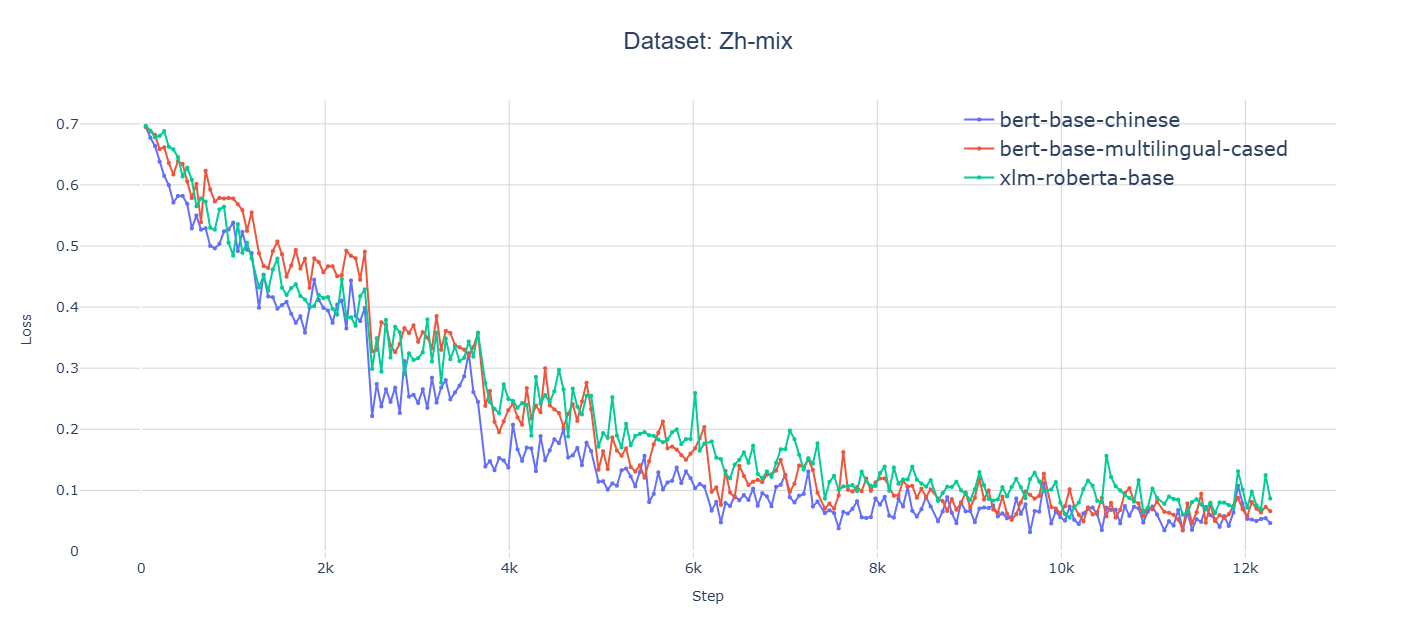
\includegraphics[width=\linewidth]{images/zh-mix.png}
        \caption{Zh-mix}
        \label{fig:en-mix}
    \end{subfigure}
    \hfill
    \begin{subfigure}[b]{0.44\linewidth}
        \centering
        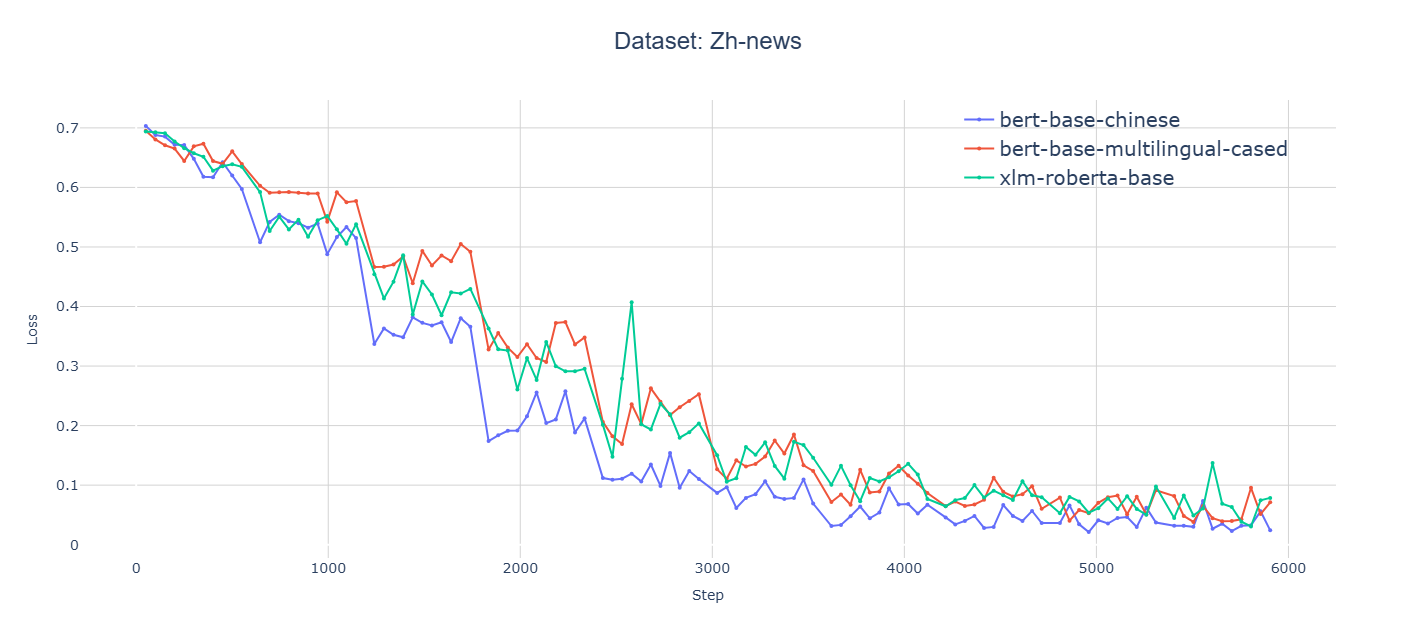
\includegraphics[width=\linewidth]{images/zh-news.png}
        \caption{Zh-news}
        \label{fig:en-essay}
    \end{subfigure}

    \vspace{-0.2em}  % 控制两行子图之间的垂直间距

    \begin{subfigure}[b]{0.44\linewidth}
        \centering
        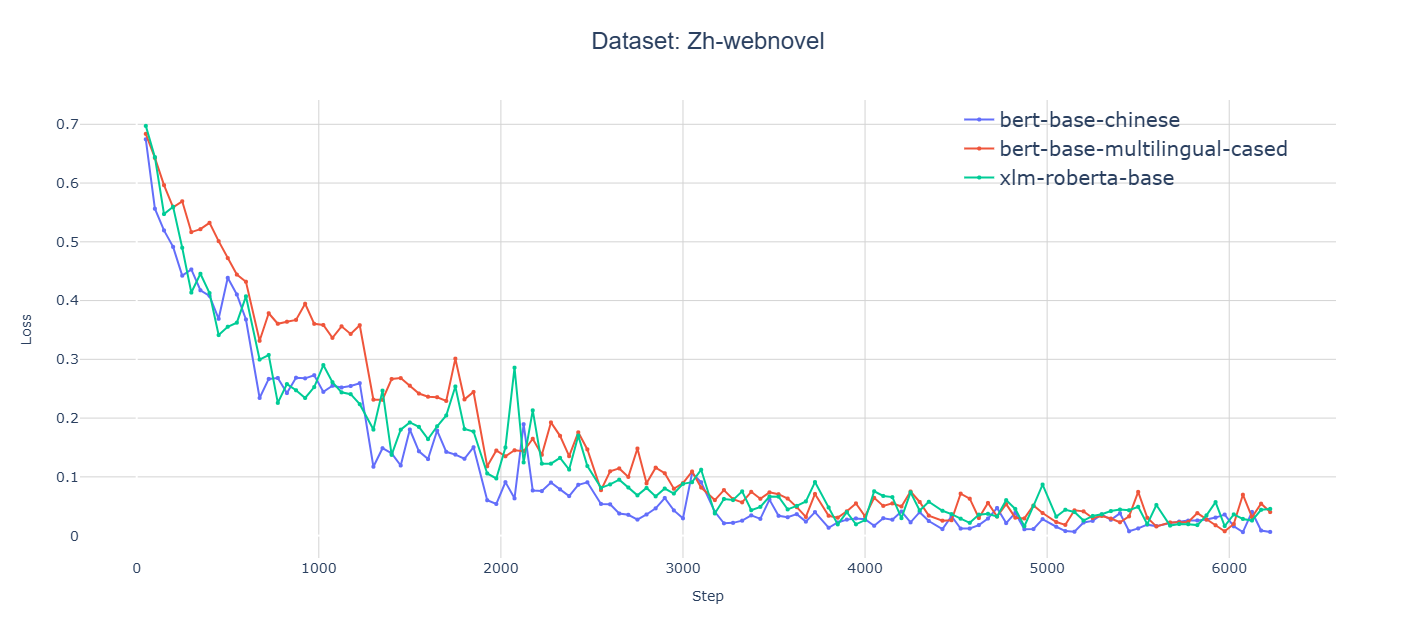
\includegraphics[width=\linewidth]{images/zh-webnovel.png}
        \caption{Zh-webnovel}
        \label{fig:en-reuter}
    \end{subfigure}
    \hfill
    \begin{subfigure}[b]{0.44\linewidth}
        \centering
        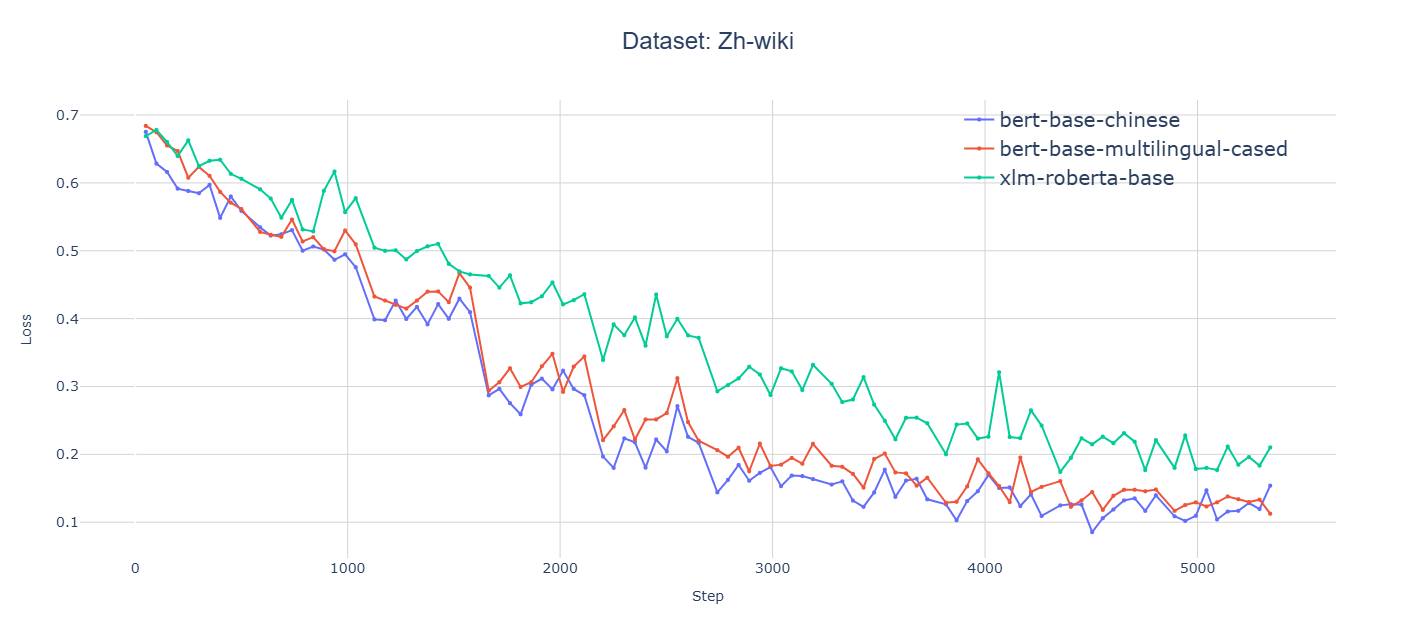
\includegraphics[width=\linewidth]{images/zh-wiki.png}
        \caption{Zh-wiki}
        \label{fig:en-wp}
    \end{subfigure}

    \label{fig:four-plots}
\end{figure}
\vspace{-0.2em}
\footnotesize
Among the three models, \textbf{bert-base-chinese} shows the fastest loss decline. All models stabilize with loss values around \textbf{0.05}, demonstrating stable and effective training.
\end{frame}


% --------------------------
\begin{frame}{Supervised Learning Method: Metrics Comparison (Zh)}

\centering
\tiny
\setlength{\tabcolsep}{2pt}
\renewcommand{\arraystretch}{1.0}

% 第一个模型:bert-base-multilingual-cased (补全wiki数据)
\resizebox{0.95\textwidth}{!}{%
\begin{tabular}{|l|c|c|c|c|}
\hline
\textbf{FT domain} & \textbf{mixed} & \textbf{webnovel} & \textbf{news} & \textbf{wiki} \\
\hline
Accuracy & 
0.7055 / 0.7880 / 0.6440 / 0.6820 & 
0.7304 / 0.9566 / 0.6272 / 0.5955 & 
0.7155 / 0.6091 / 0.6031 / 0.9517 & 
0.6820 / 0.6091 / 0.6031 / 0.9517 \\
\hline
Precision & 
0.6818 / 0.7238 / 0.6289 / 0.6998 & 
0.6722 / 0.9190 / 0.5997 / 0.5952 & 
0.6924 / 0.5681 / 0.6009 / 0.9602 & 
0.6998 / 0.5681 / 0.6009 / 0.9602 \\
\hline
Recall & 
0.8447 / 0.9056 / 0.8226 / 0.8125 & 
0.9701 / 0.9979 / 0.9201 / 0.9943 & 
0.8441 / 0.7876 / 0.7778 / 0.9583 & 
0.8125 / 0.7876 / 0.7778 / 0.9583 \\
\hline
F1 Score & 
0.7546 / 0.8046 / 0.7128 / 0.7520 & 
0.7941 / 0.9568 / 0.7262 / 0.7447 & 
0.7608 / 0.6601 / 0.6780 / 0.9592 & 
0.7520 / 0.6601 / 0.6780 / 0.9592 \\
\hline
AUROC & 
0.7961 / 0.8879 / 0.6976 / 0.7649 & 
0.7528 / 0.9988 / 0.6629 / 0.5219 & 
0.7881 / 0.6637 / 0.6390 / 0.9936 & 
0.7649 / 0.6637 / 0.6390 / 0.9936 \\
\hline
\end{tabular}%
}

\vspace{0.2cm}
{\scriptsize \captionof{table}{bert-base-multilingual-cased (Zh) overall/webnovel/news/wiki}}

\vspace{0.5cm}

% 第二个模型:bert-base-chinese
\resizebox{0.95\textwidth}{!}{%
\begin{tabular}{|l|c|c|c|c|}
\hline
\textbf{FT domain} & \textbf{mixed} & \textbf{webnovel} & \textbf{news} & \textbf{wiki} \\
\hline
Accuracy & 
0.7219 / 0.7942 / 0.6754 / 0.6933 & 
0.7376 / 0.9835 / 0.6188 / 0.5978 & 
0.7920 / 0.7384 / 0.9717 / 0.6573 & 
0.7564 / 0.7198 / 0.6272 / 0.9348 \\
\hline
Precision & 
0.6893 / 0.7236 / 0.6452 / 0.7060 & 
0.6741 / 0.9668 / 0.5869 / 0.5977 & 
0.7511 / 0.6814 / 0.9500 / 0.6573 & 
0.7251 / 0.7010 / 0.6008 / 0.9181 \\
\hline
Recall & 
0.8759 / 0.9270 / 0.8791 / 0.8277 & 
0.9841 / 1.0000 / 0.9805 / 0.9848 & 
0.9151 / 0.8584 / 1.0000 / 0.8826 & 
0.8786 / 0.7296 / 0.9123 / 0.9773 \\
\hline
F1 Score & 
0.7715 / 0.8128 / 0.7442 / 0.7620 & 
0.8014 / 0.9831 / 0.7343 / 0.7439 & 
0.8250 / 0.7767 / 0.9744 / 0.6869 & 
0.7945 / 0.7150 / 0.7457 / 0.9468 \\
\hline
AUROC & 
0.8271 / 0.9125 / 0.7516 / 0.7920 & 
0.7549 / 0.9999 / 0.7053 / 0.5985 & 
0.8396 / 0.7989 / 0.9950 / 0.7081 & 
0.8328 / 0.7817 / 0.6977 / 0.9927 \\
\hline
\end{tabular}%
}

\vspace{0.2cm}
{\scriptsize \captionof{table}{bert-base-chinese (Zh) overall/webnovel/news/wiki}}

\vspace{0.5cm}

% 第三个模型:xlm-roberta-base
\resizebox{0.95\textwidth}{!}{%
\begin{tabular}{|l|c|c|c|c|}
\hline
\textbf{FT domain} & \textbf{mixed} & \textbf{webnovel} & \textbf{news} & \textbf{wiki} \\
\hline
Accuracy & 
0.7774 / 0.8676 / 0.7309 / 0.7292 & 
0.6849 / 0.8387 / 0.5979 / 0.6112 & 
0.7784 / 0.7466 / 0.9277 / 0.6528 & 
0.7610 / 0.7218 / 0.6565 / 0.9157 \\
\hline
Precision & 
0.7479 / 0.8062 / 0.6975 / 0.7487 & 
0.6324 / 0.7566 / 0.5734 / 0.6056 & 
0.7656 / 0.6751 / 0.8868 / 0.7386 & 
0.7158 / 0.6518 / 0.6190 / 0.9450 \\
\hline
Recall & 
0.8819 / 0.9549 / 0.8811 / 0.8182 & 
0.9841 / 0.9807 / 0.9825 / 0.9886 & 
0.8454 / 0.9142 / 0.9922 / 0.9376 & 
0.9190 / 0.9077 / 0.9376 / 0.9110 \\
\hline
F1 Score & 
0.8094 / 0.8743 / 0.7786 / 0.7819 & 
0.7700 / 0.8542 / 0.7241 / 0.7511 & 
0.8035 / 0.7767 / 0.9365 / 0.6869 & 
0.8048 / 0.7587 / 0.7457 / 0.9277 \\
\hline
AUROC & 
0.8751 / 0.9531 / 0.8099 / 0.8259 & 
0.7549 / 0.9704 / 0.7112 / 0.5307 & 
0.8685 / 0.8667 / 0.9910 / 0.7081 & 
0.8304 / 0.8204 / 0.7144 / 0.9831 \\
\hline
\end{tabular}%
}

\vspace{0.2cm}
{\scriptsize \captionof{table}{xlm-roberta-base (Zh) overall/webnovel/news/wiki}}

\end{frame}

\begin{frame}{Supervised Learning Method(Spectrum)(Eng): In domain}
    \begin{figure}
        \centering
        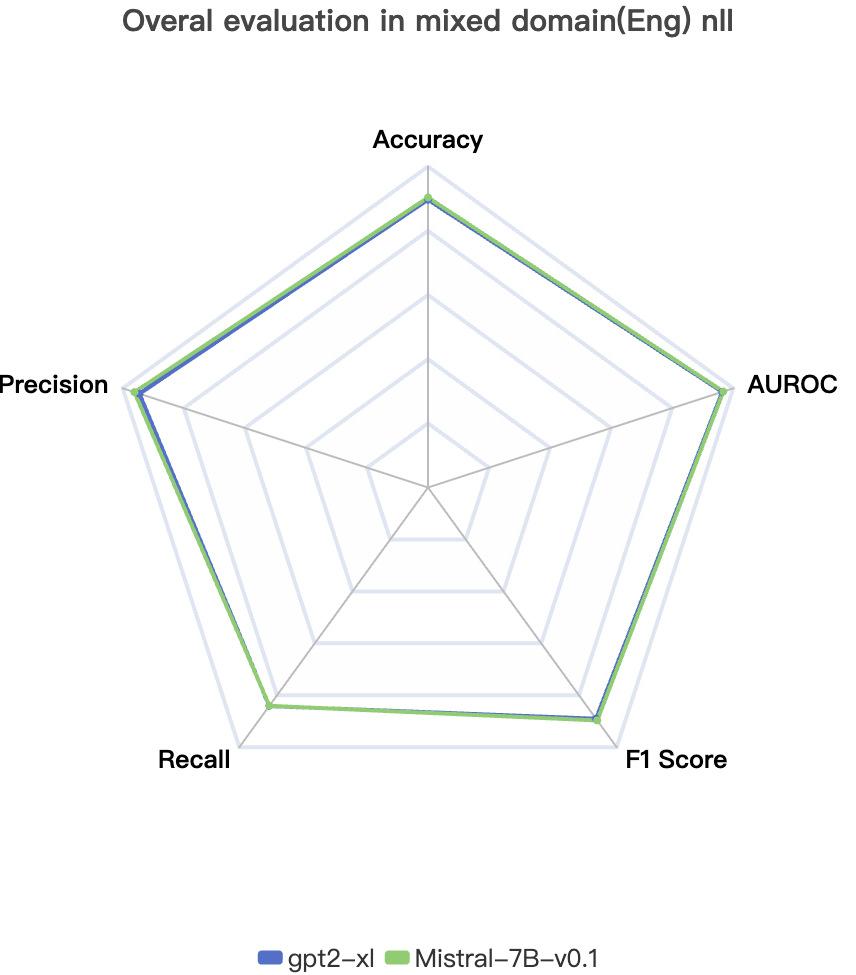
\includegraphics[width=0.5\linewidth]{images/Overal evaluation in mixed domain(Eng) nll.png}
        \label{fig:enter-label}
    \end{figure}
    \vspace{-0.2em}
\begin{flushleft}
\scriptsize
In the English mixed domain, the metrics of the two models are almost identical.
\normalize
\end{flushleft}
\end{frame}

\begin{frame}{Supervised Learning Method(Spectrum)(Eng):OOD}
\begin{columns}[t]
  \column{0.33\textwidth}
    \centering
    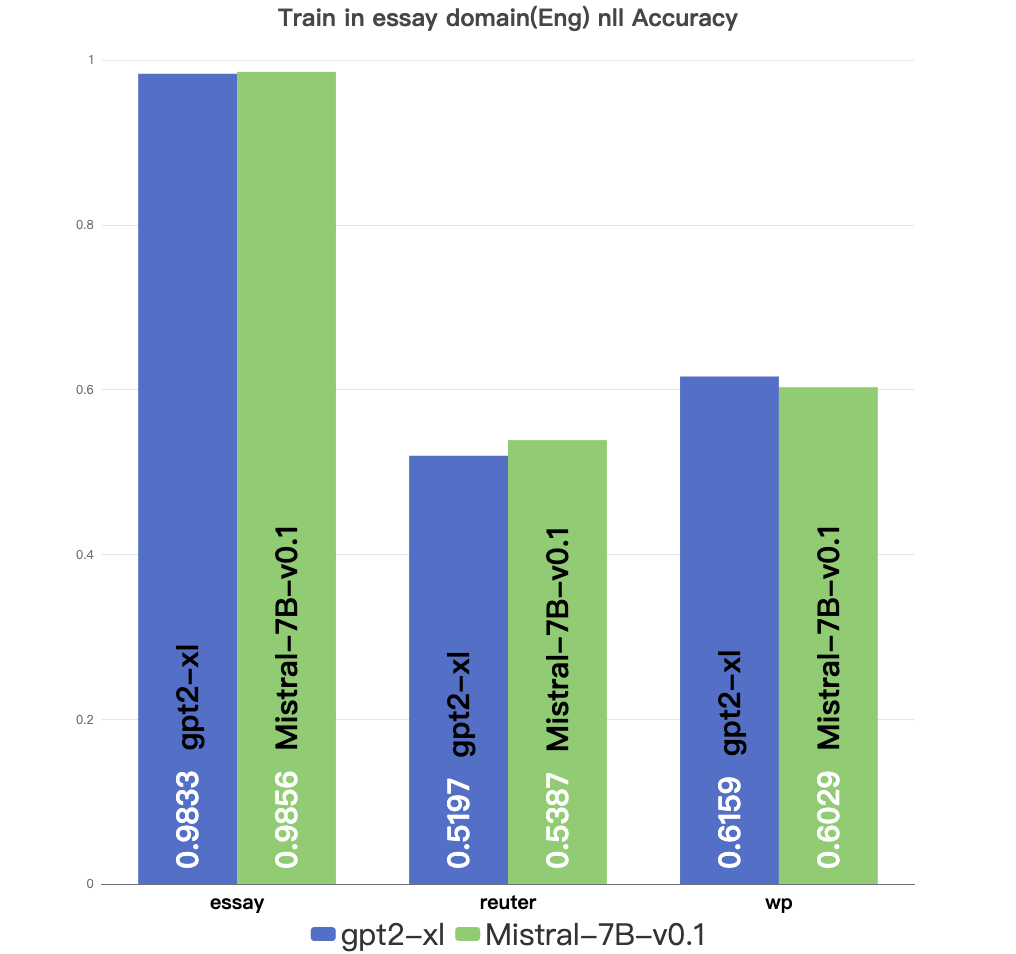
\includegraphics[width=\linewidth]{images/Train in essay domain(Eng) nll Accuracy.png}
    \caption*{Essay}

  \column{0.33\textwidth}
    \centering
    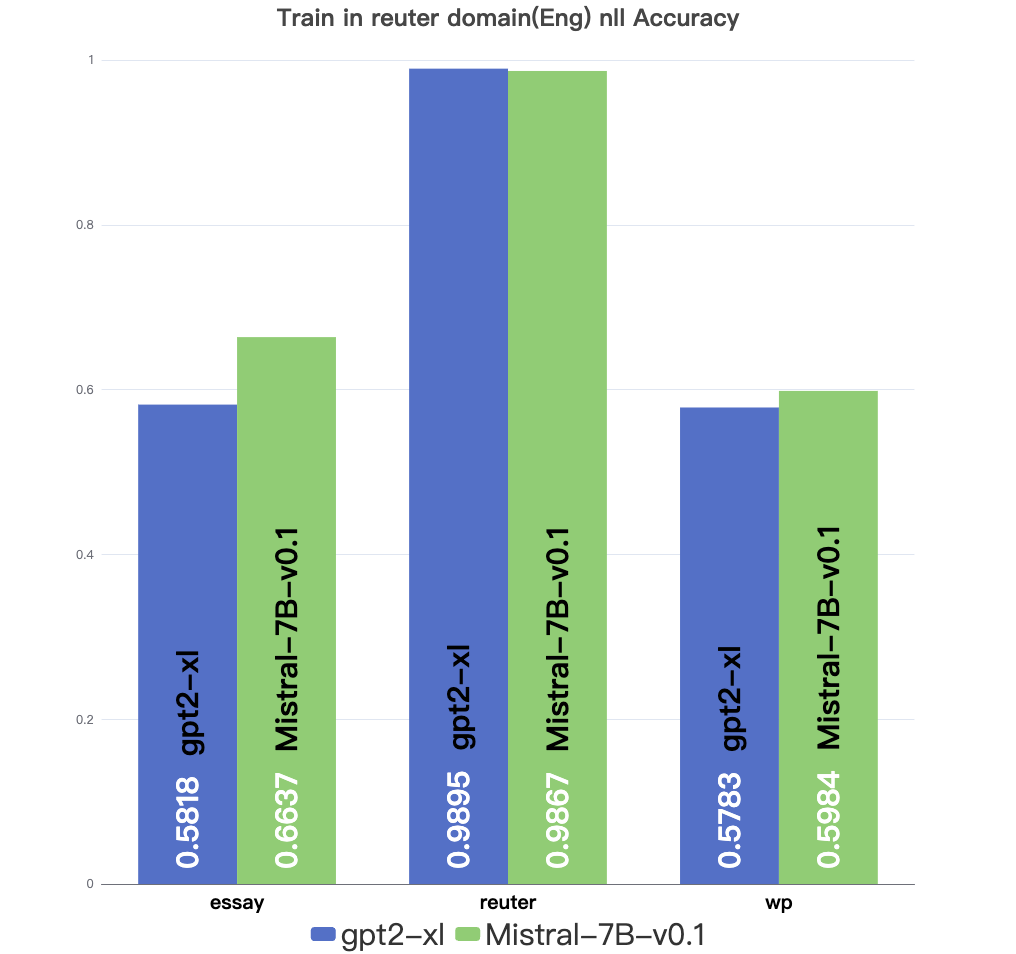
\includegraphics[width=\linewidth]{images/Train in reuter domain(Eng) nll Accuracy.png}
    \caption*{Reuter}

  \column{0.33\textwidth}
    \centering
    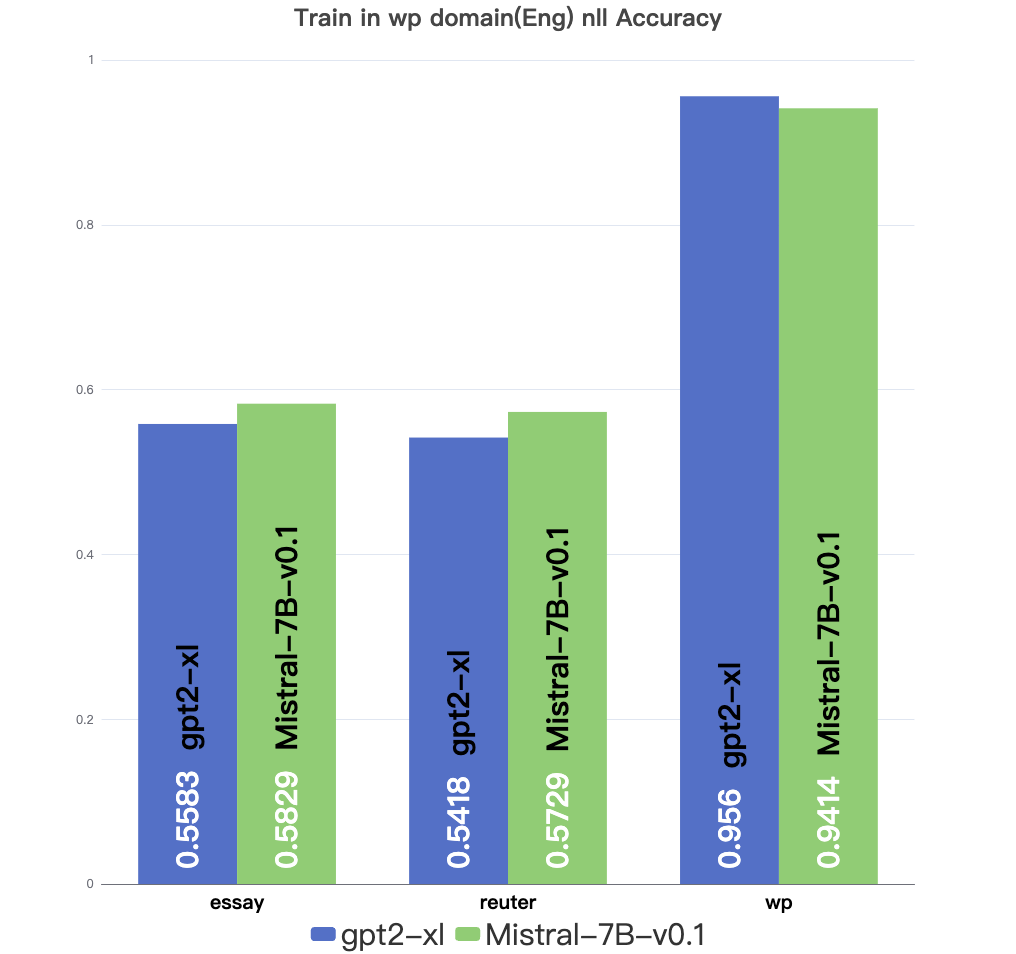
\includegraphics[width=\linewidth]{images/Train in wp domain(Eng) nll Accuracy.png}
    \caption*{Wp}
\end{columns}
\begin{itemize}
    \item Perform well within their \textbf{own training domain}, \textbf{above 0.95}
    \item Accuracy significantly decreases when \textbf{tested on other domains}, often dropping \textbf{below 0.6}
    \item Among the two models, \textbf{Mistral-7B-v0.1} shows relatively better generalization across different domains.
    
\end{itemize}
\end{frame}


\begin{frame}{Supervised Learning Method(Spectrum)(Zh):In domain}
    \begin{figure}
        \centering
        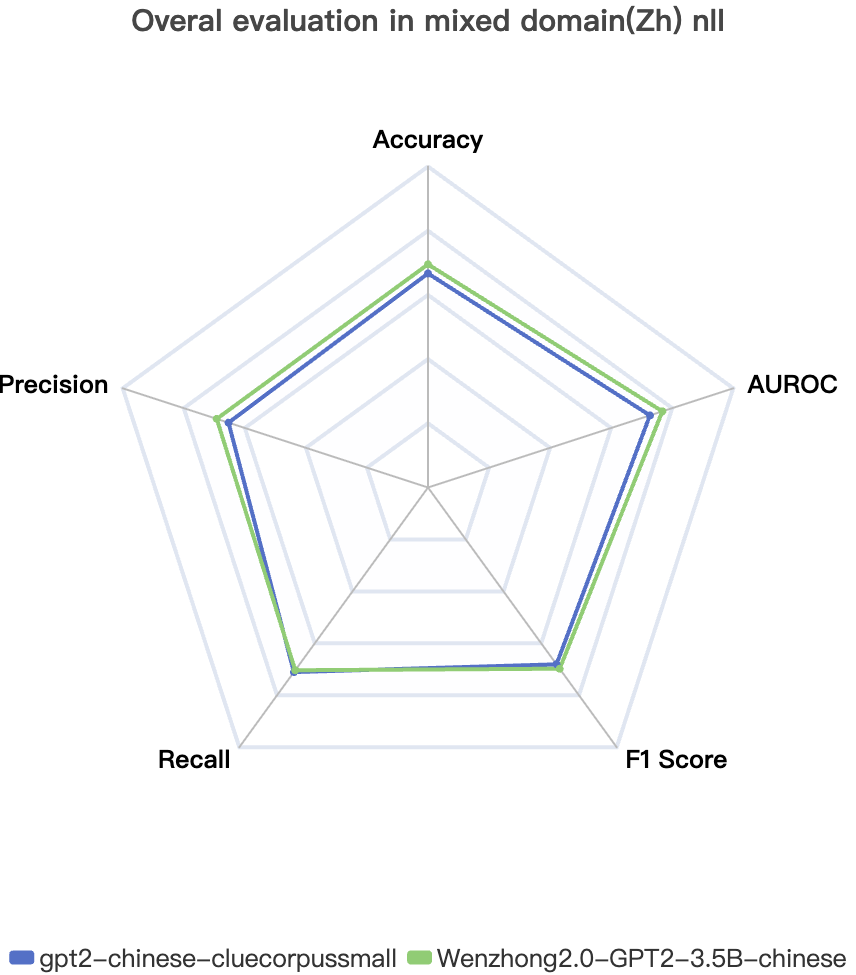
\includegraphics[width=0.5\linewidth]{images/Overal evaluation in mixed domain(Zh) nll.png}
        \label{fig:enter-label}
    \end{figure}
    \vspace{-0.2em}
\begin{flushleft}
\scriptsize
In the Chinese mixed domain, \textbf{Wenzhong2.0-GPT2-3.5B-chinese} performs better across most metrics except recall.
\normalize
\end{flushleft}
\end{frame}

\begin{frame}{Supervised Learning Method(Spectrum)(Zh):OOD}
\begin{columns}[t]
  \column{0.33\textwidth}
    \centering
    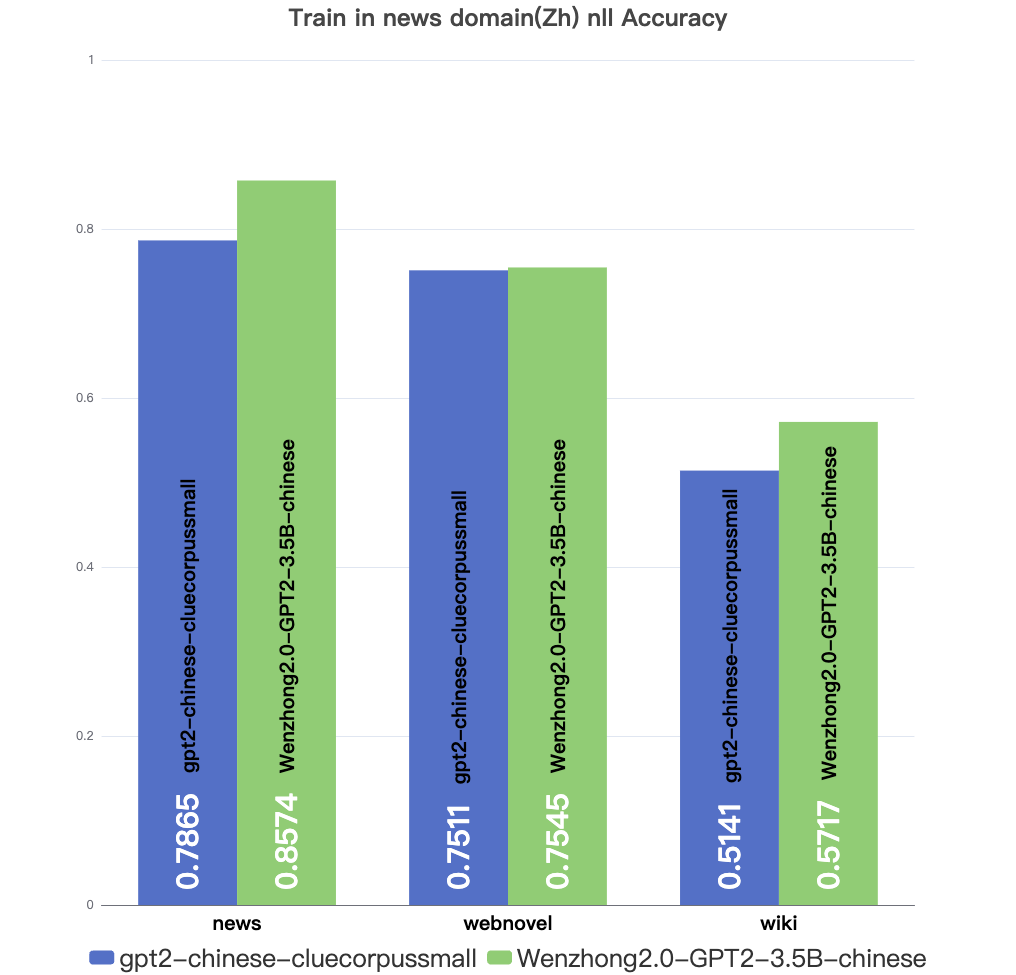
\includegraphics[width=\linewidth]{images/Train in news domain(Zh) nll Accuracy.png}
    \caption*{News}

  \column{0.33\textwidth}
    \centering
    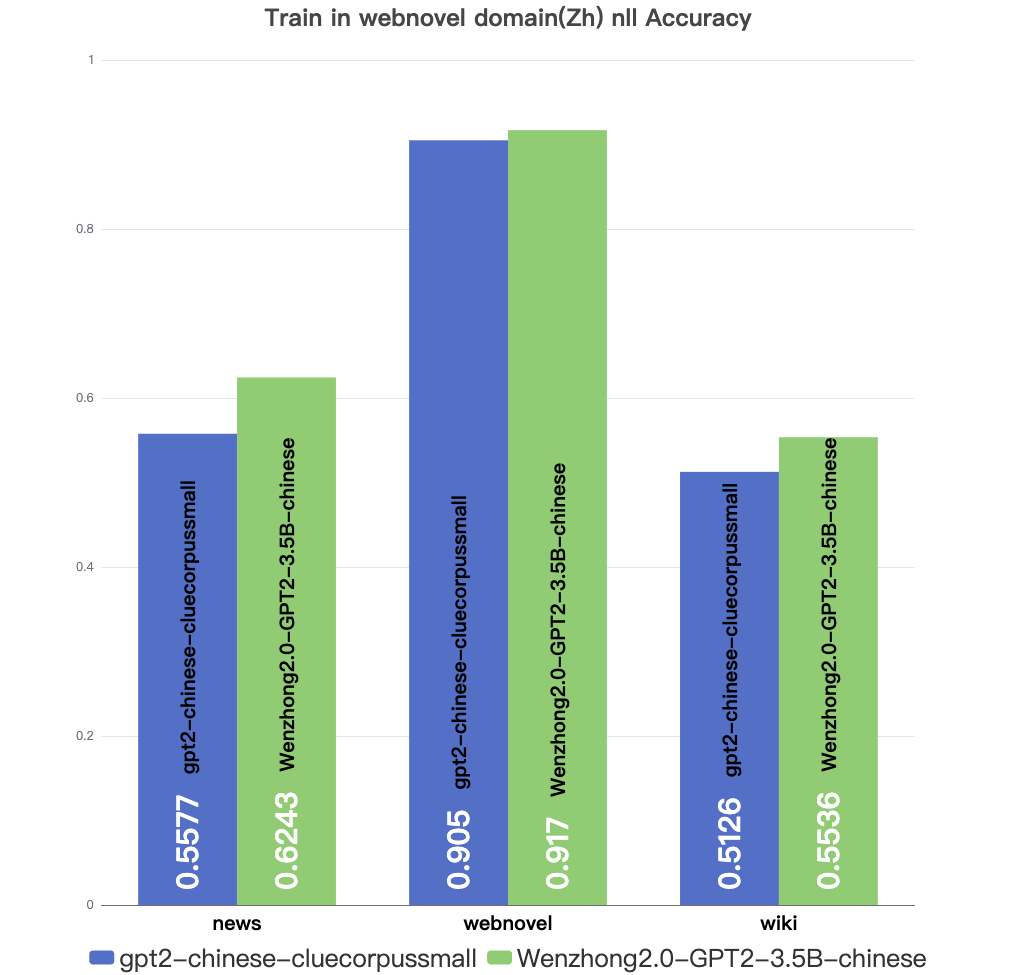
\includegraphics[width=\linewidth]{images/Train in webnovel domain(Zh) nll Accuracy.png}
    \caption*{Webnovel}

  \column{0.33\textwidth}
    \centering
    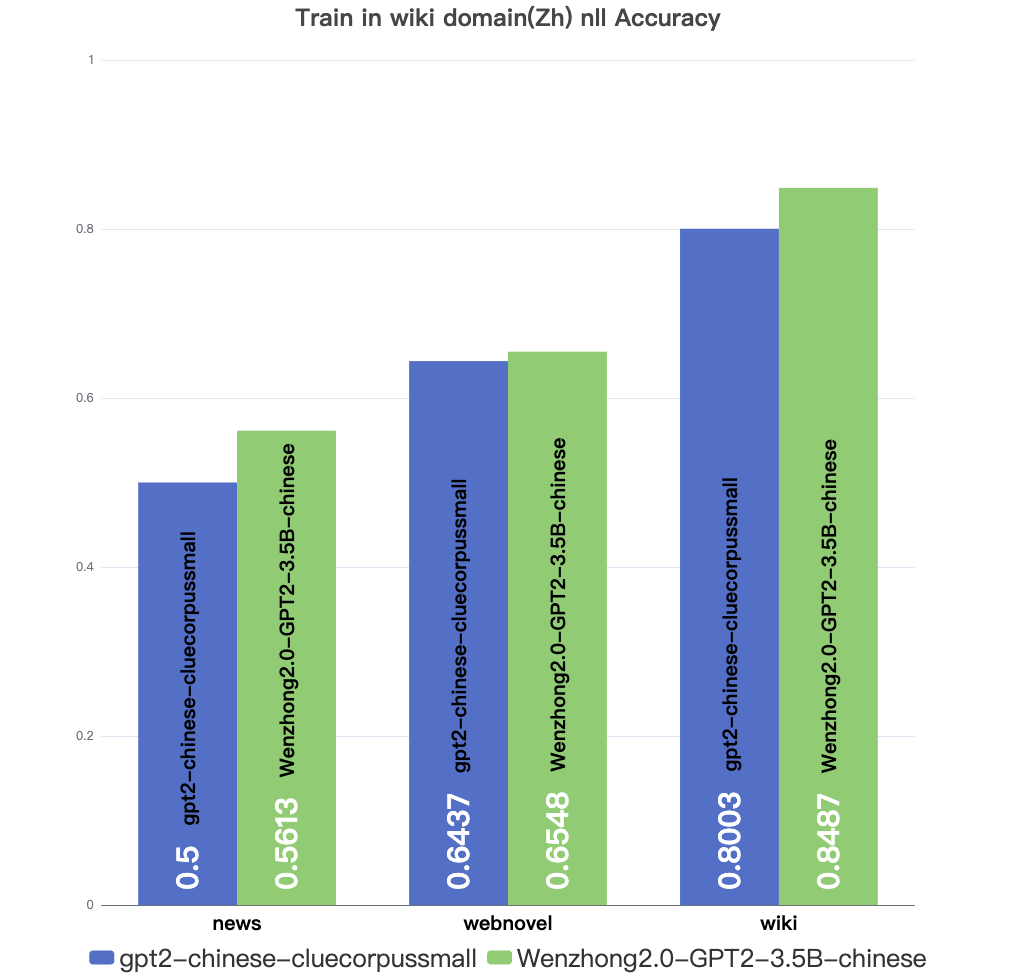
\includegraphics[width=\linewidth]{images/Train in wiki domain(Zh) nll Accuracy.png}
    \caption*{Wiki}
\end{columns}
\begin{itemize}
    \item Perform well within their \textbf{own training domain}, \textbf{above 0.8}
    \item Accuracy significantly decreases when \textbf{tested on other domains}, often dropping \textbf{below 0.6}
    \item Among the two models, \textbf{Wenzhong2.0-GPT2-3.5B-chinese} shows relatively better generalization across different domains.
    
\end{itemize}
\end{frame}


% --------------------------
\begin{frame}{Zero-shot Detection:Aggregated Power Spectrum}
\begin{columns}[t]
  \column{0.2\textwidth}
    \centering
    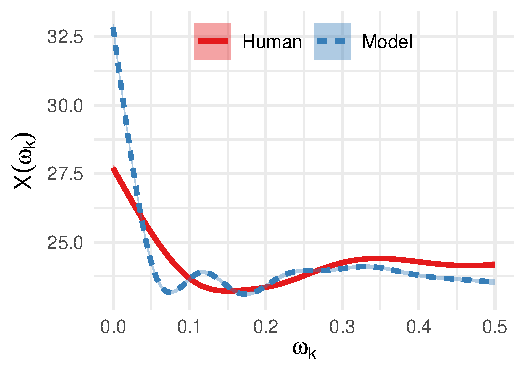
\includegraphics[width=\linewidth]{images/en_essay_aggregated.pdf}
    
    {\scriptsize \textbf{k=5, higher=model}}

  \column{0.2\textwidth}
    \centering
    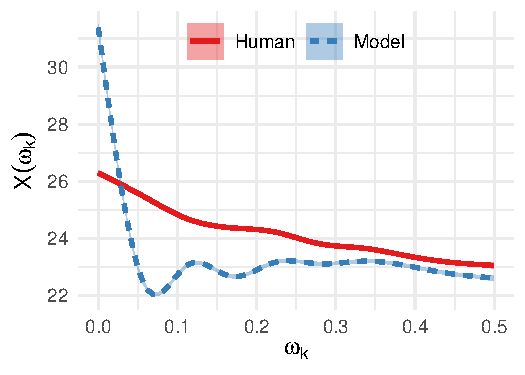
\includegraphics[width=\linewidth]{images/en_reuter_aggregated.pdf}
    
    {\scriptsize \textbf{k=5, higher=model}}

  \column{0.2\textwidth}
    \centering
    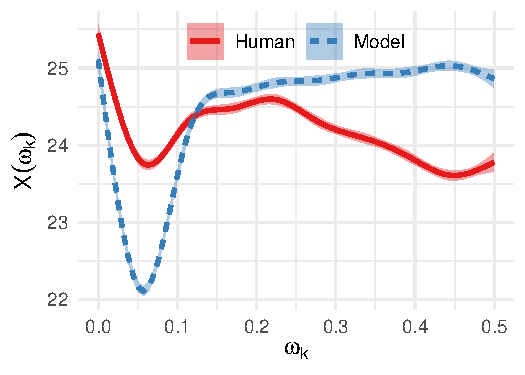
\includegraphics[width=\linewidth]{images/eng_wp_aggregated.pdf}
    
    {\scriptsize \textbf{k=3, higher=model}}
\end{columns}

\vspace{0.3cm}

\begin{columns}[t]
  \column{0.2\textwidth}
    \centering
    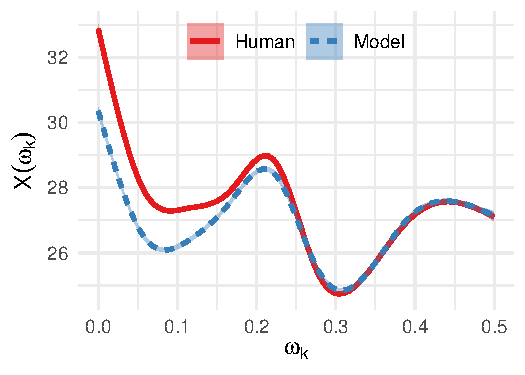
\includegraphics[width=\linewidth]{images/zh_news_aggregated.pdf}
    {\scriptsize \textbf{k=46, higher=human}}

  \column{0.2\textwidth}
    \centering
    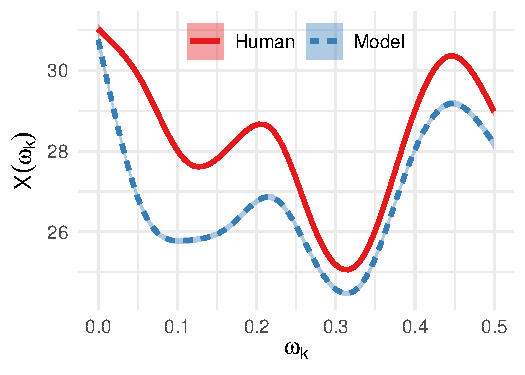
\includegraphics[width=\linewidth]{images/zh_webnovel_aggregated.pdf}
    {\scriptsize \textbf{k=50, higher=human}}

  \column{0.2\textwidth}
    \centering
    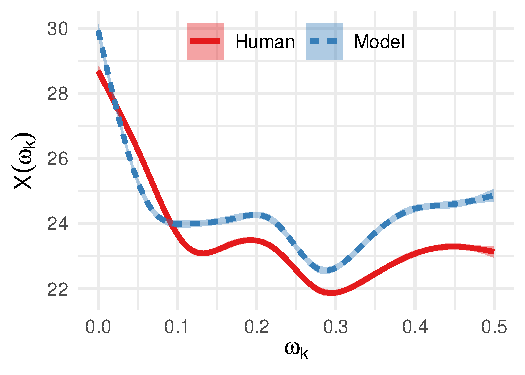
\includegraphics[width=\linewidth]{images/zh_wiki_aggregated.pdf}
    {\scriptsize \textbf{k=49, higher=human}}
\end{columns}

\begin{itemize}
    \item For English texts, model can distinguish between hm and llm texts using only \textbf{a small number of low-frequency} features.
    \item For \textbf{English} texts, the llm text has \textbf{higher} power than the hm text while for \textbf{Chinese}, where llm text has \textbf{lower} power..
\end{itemize}

\end{frame}
%----------------------------------
\begin{frame}{Zero-shot Detection (Eng)}

\centering
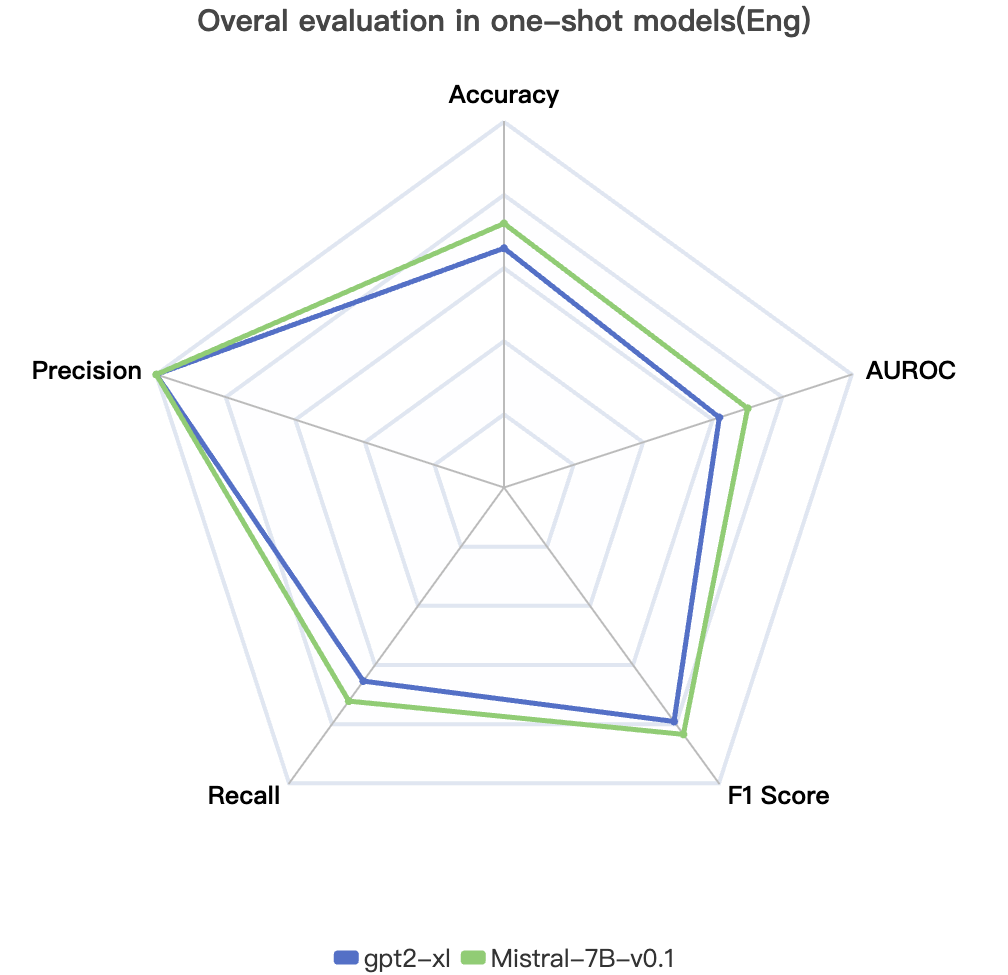
\includegraphics[width=0.5\textwidth]{images/Overal evaluation in one-shot models(Eng).png}

\vspace{-0.2em}
\begin{flushleft}
\scriptsize
\textbf{Mistral-7B-v0.1} slightly outperforms gpt2-xl across most metrics in one-shot detection for English texts.
\normalize
\end{flushleft}

\end{frame}

%--------------------
\begin{frame}{Zero-shot Detection:Accuracy (Eng)}
    \begin{figure}
        \centering
        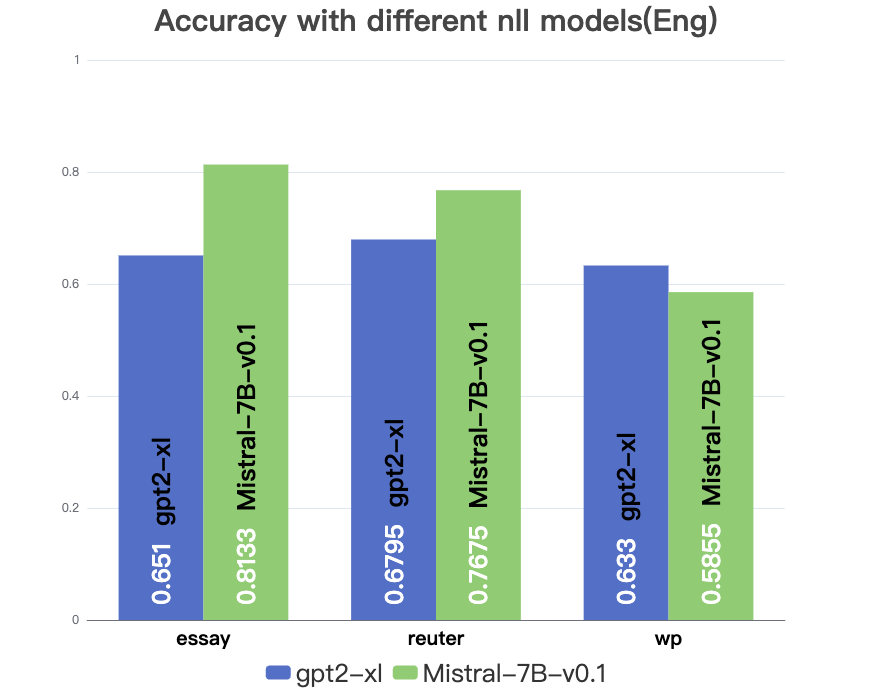
\includegraphics[width=0.5\linewidth]{images/Accuracy with different nll models(Eng).png}
        \label{fig:enter-label}
    \end{figure}
    \begin{itemize}
    \item \textbf{Mistral-7B-v0.1} Outperforms GPT2-XL in Essay and Reuter Domains(\textbf{both above 0.75})
    \item Both Models \textbf{Struggle} on the wp Domain(\textbf{0.63 and 0.59})
    \item \textbf{Mistral-7B-v0.1} generate \textbf{better nll}
\end{itemize}
\end{frame}


\begin{frame}{Zero-shot Detection:AUROC curve (Eng)}
\begin{columns}[t]
  \column{0.2\textwidth}
    \centering
    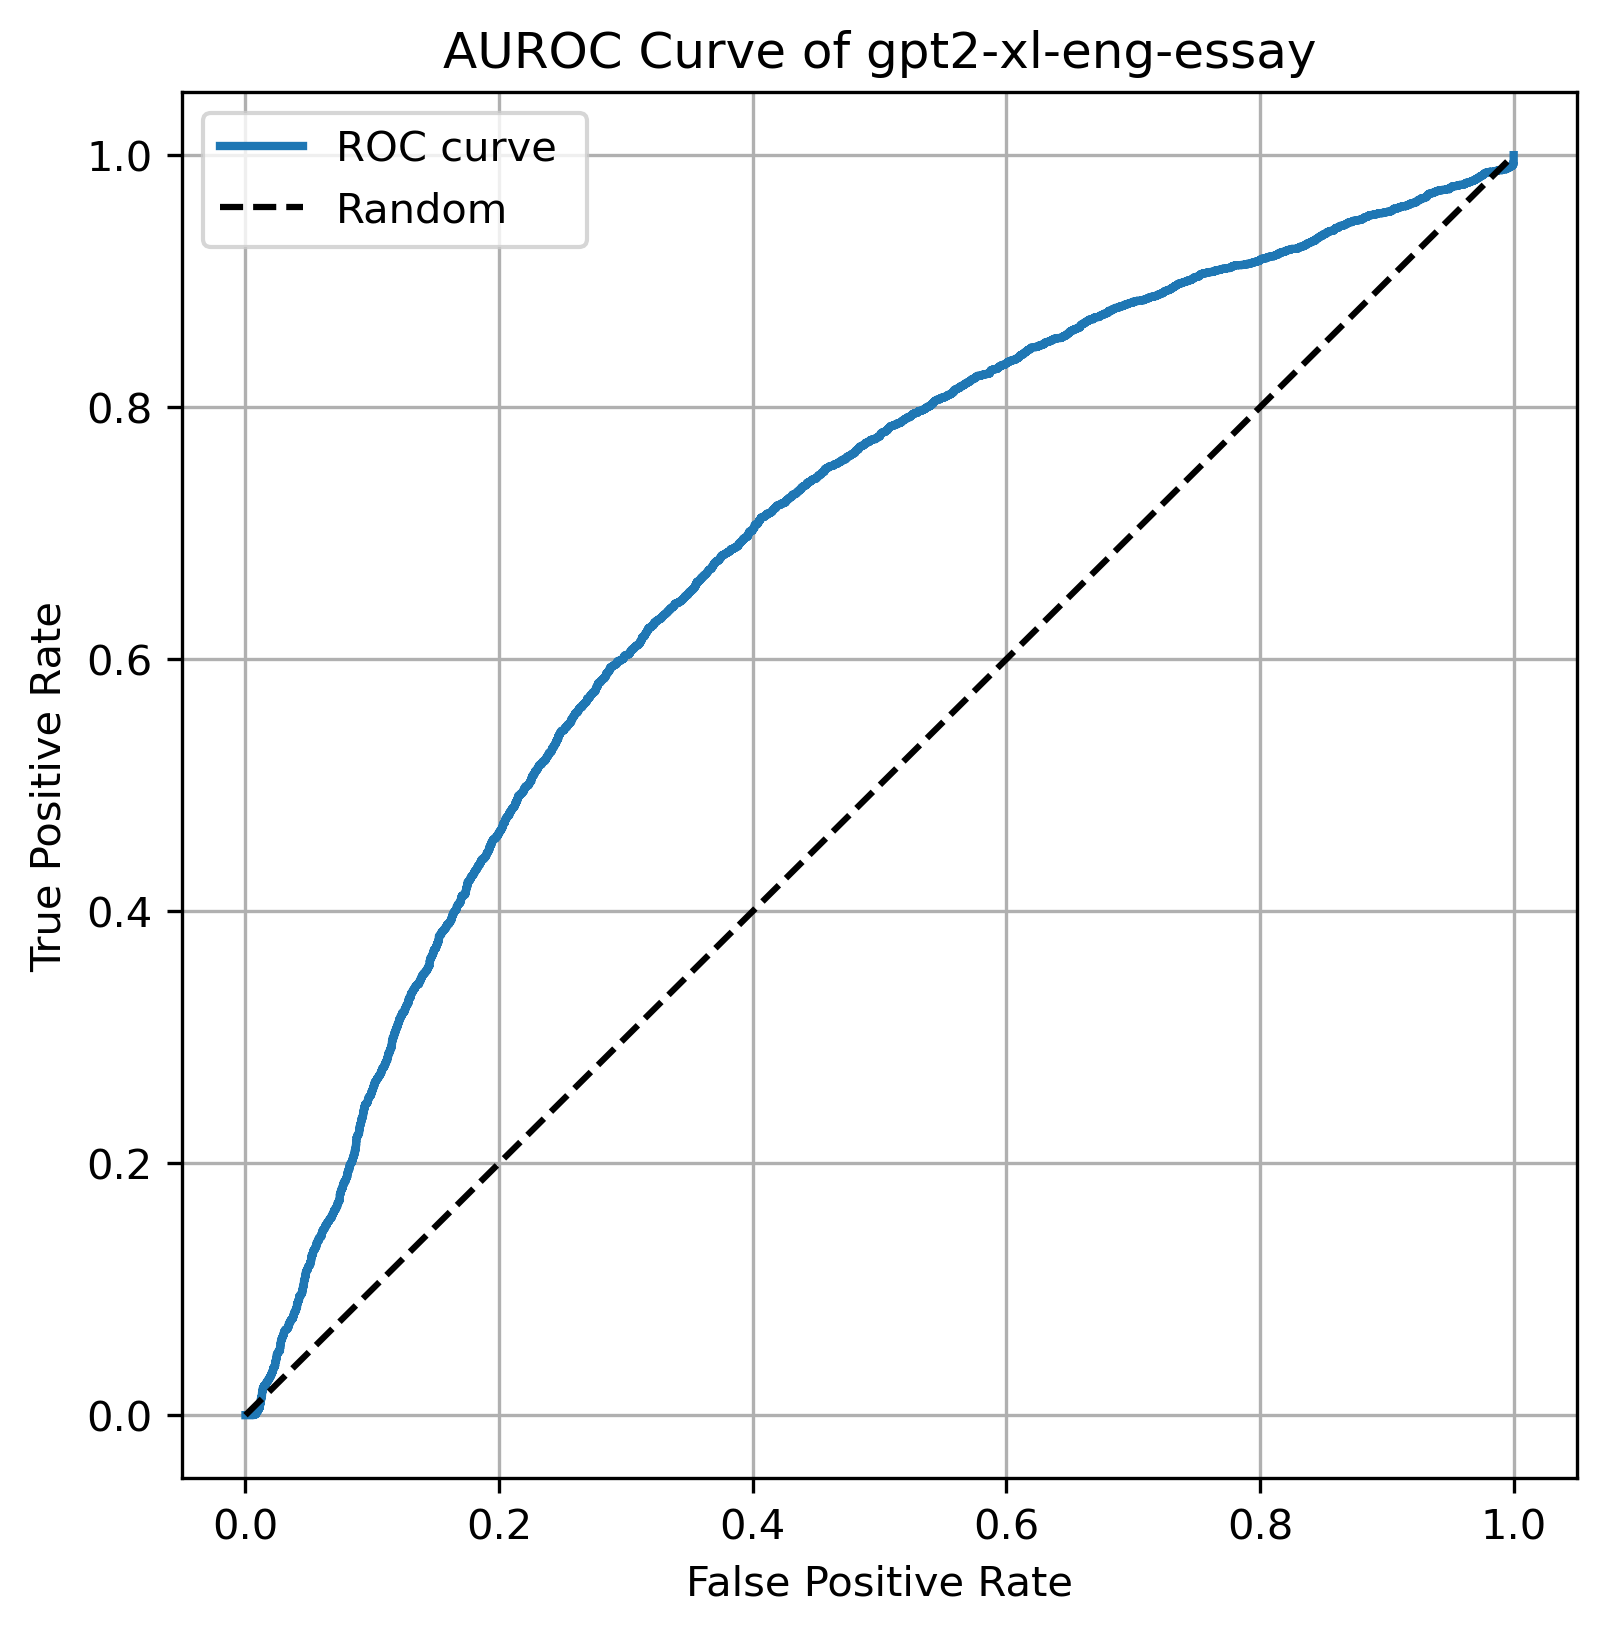
\includegraphics[width=\linewidth]{images/gpt2-xl-eng-essay.png}

  \column{0.2\textwidth}
    \centering
    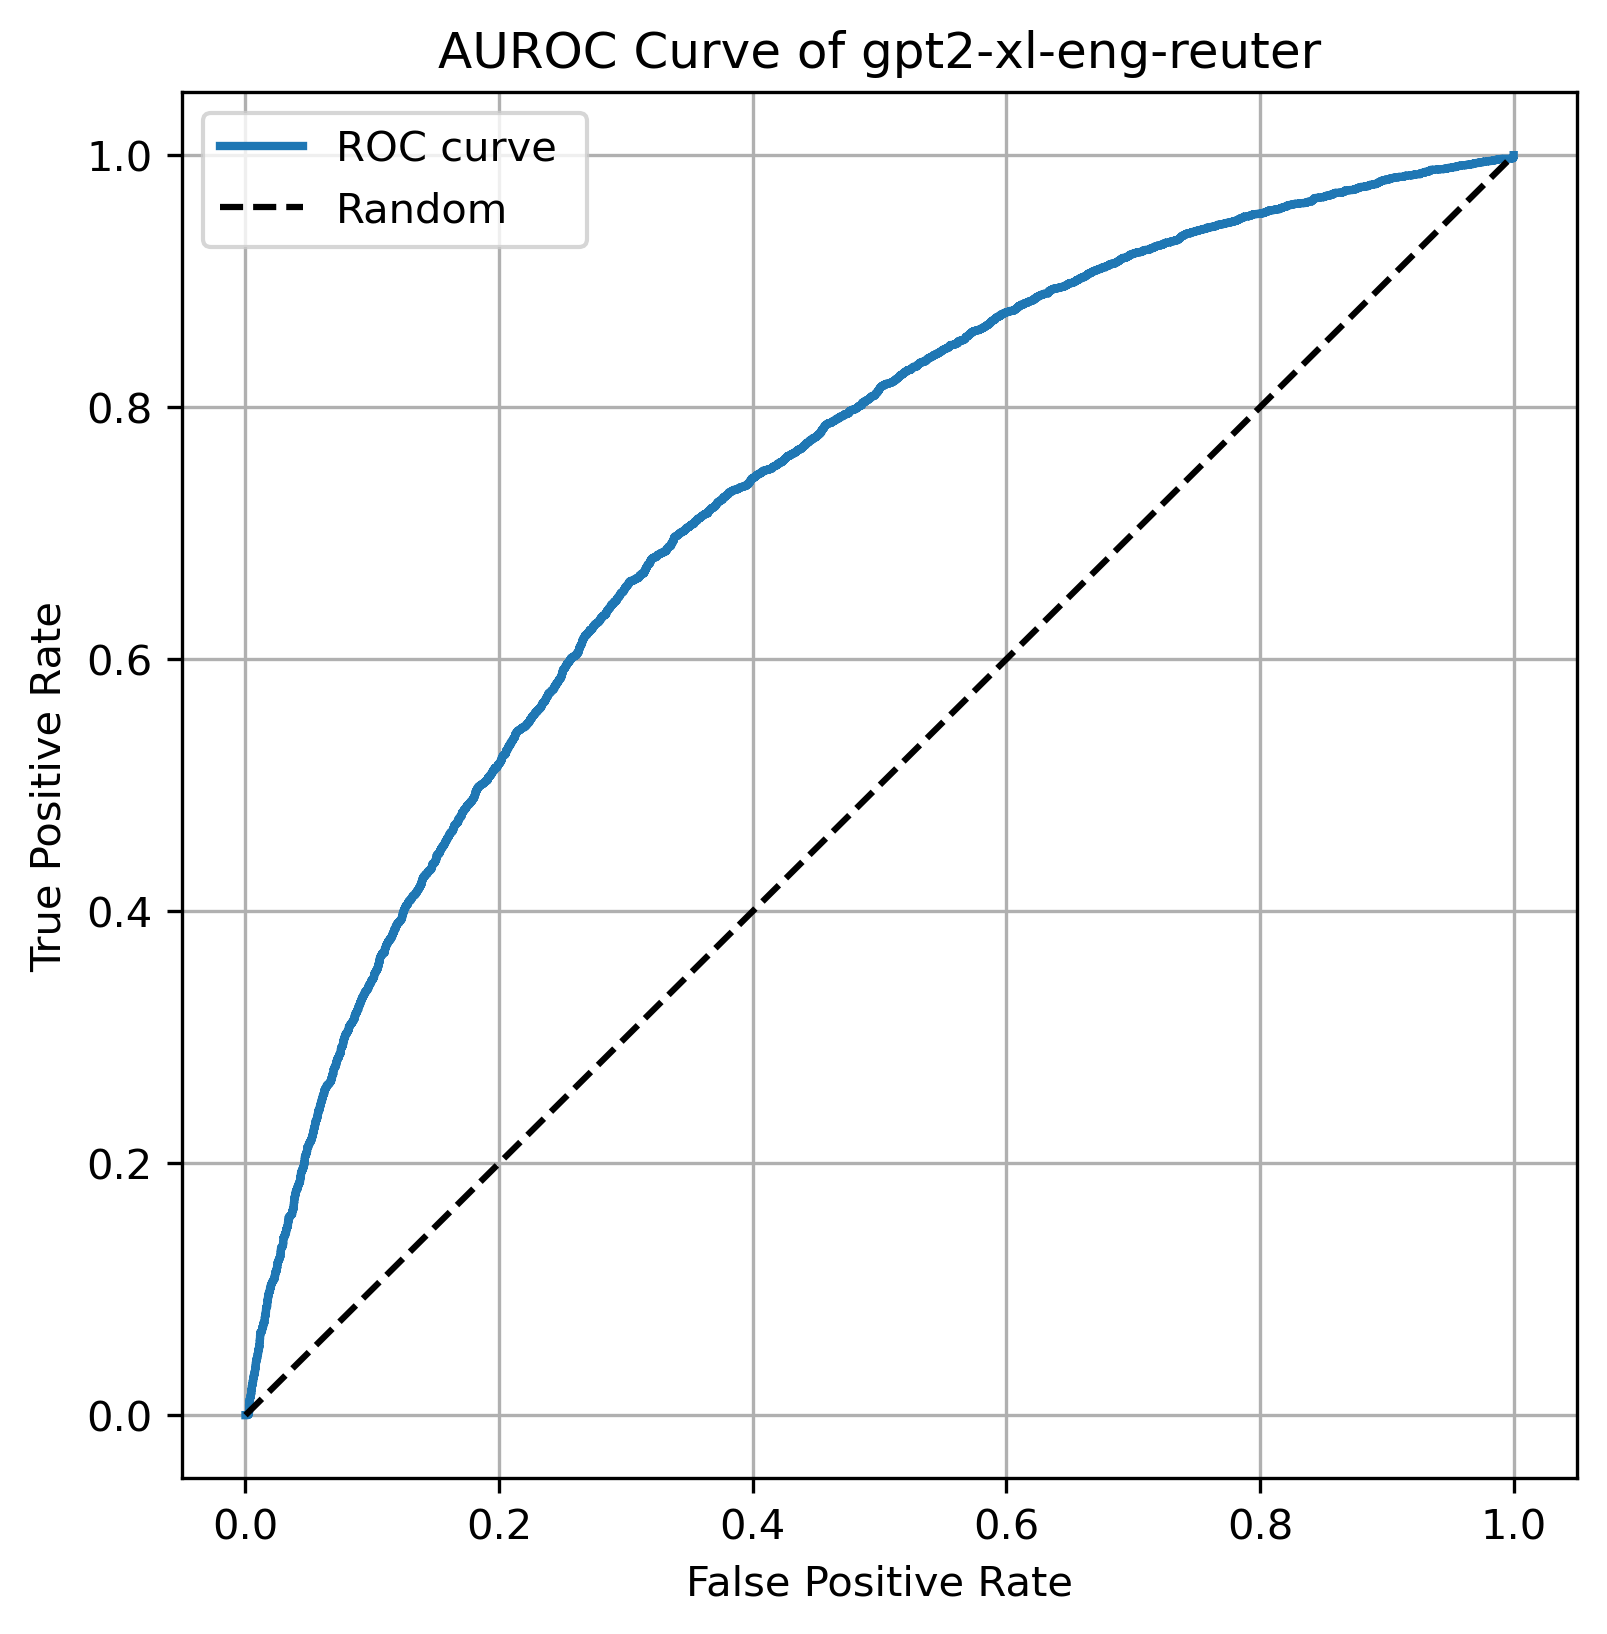
\includegraphics[width=\linewidth]{images/gpt2-xl-eng-reuter.png}

  \column{0.2\textwidth}
    \centering
    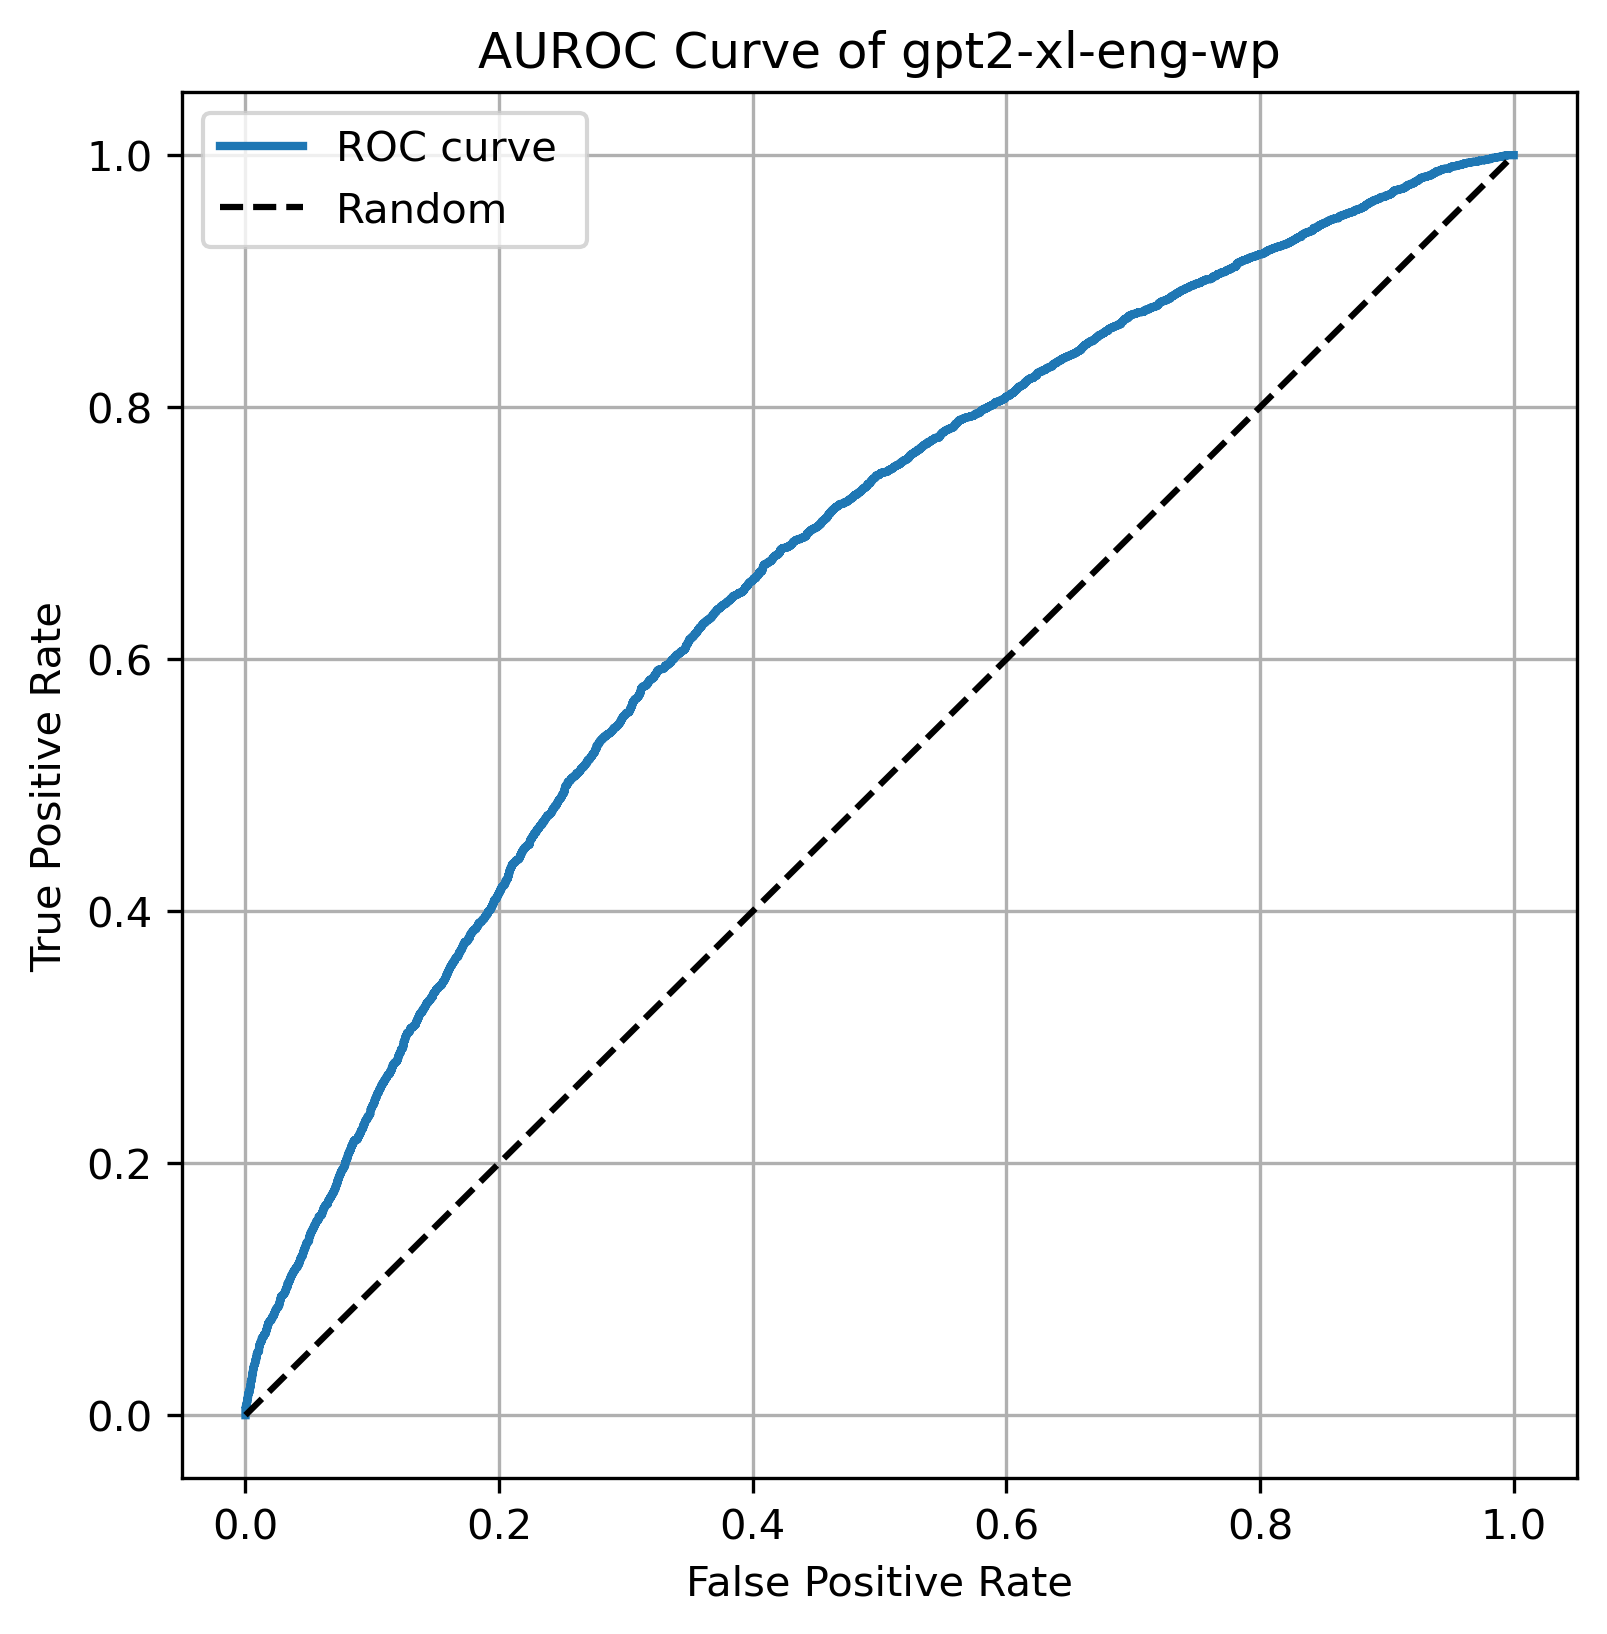
\includegraphics[width=\linewidth]{images/gpt2-xl-eng-wp.png}
\end{columns}

\vspace{0.3cm}

\begin{columns}[t]
  \column{0.2\textwidth}
    \centering
    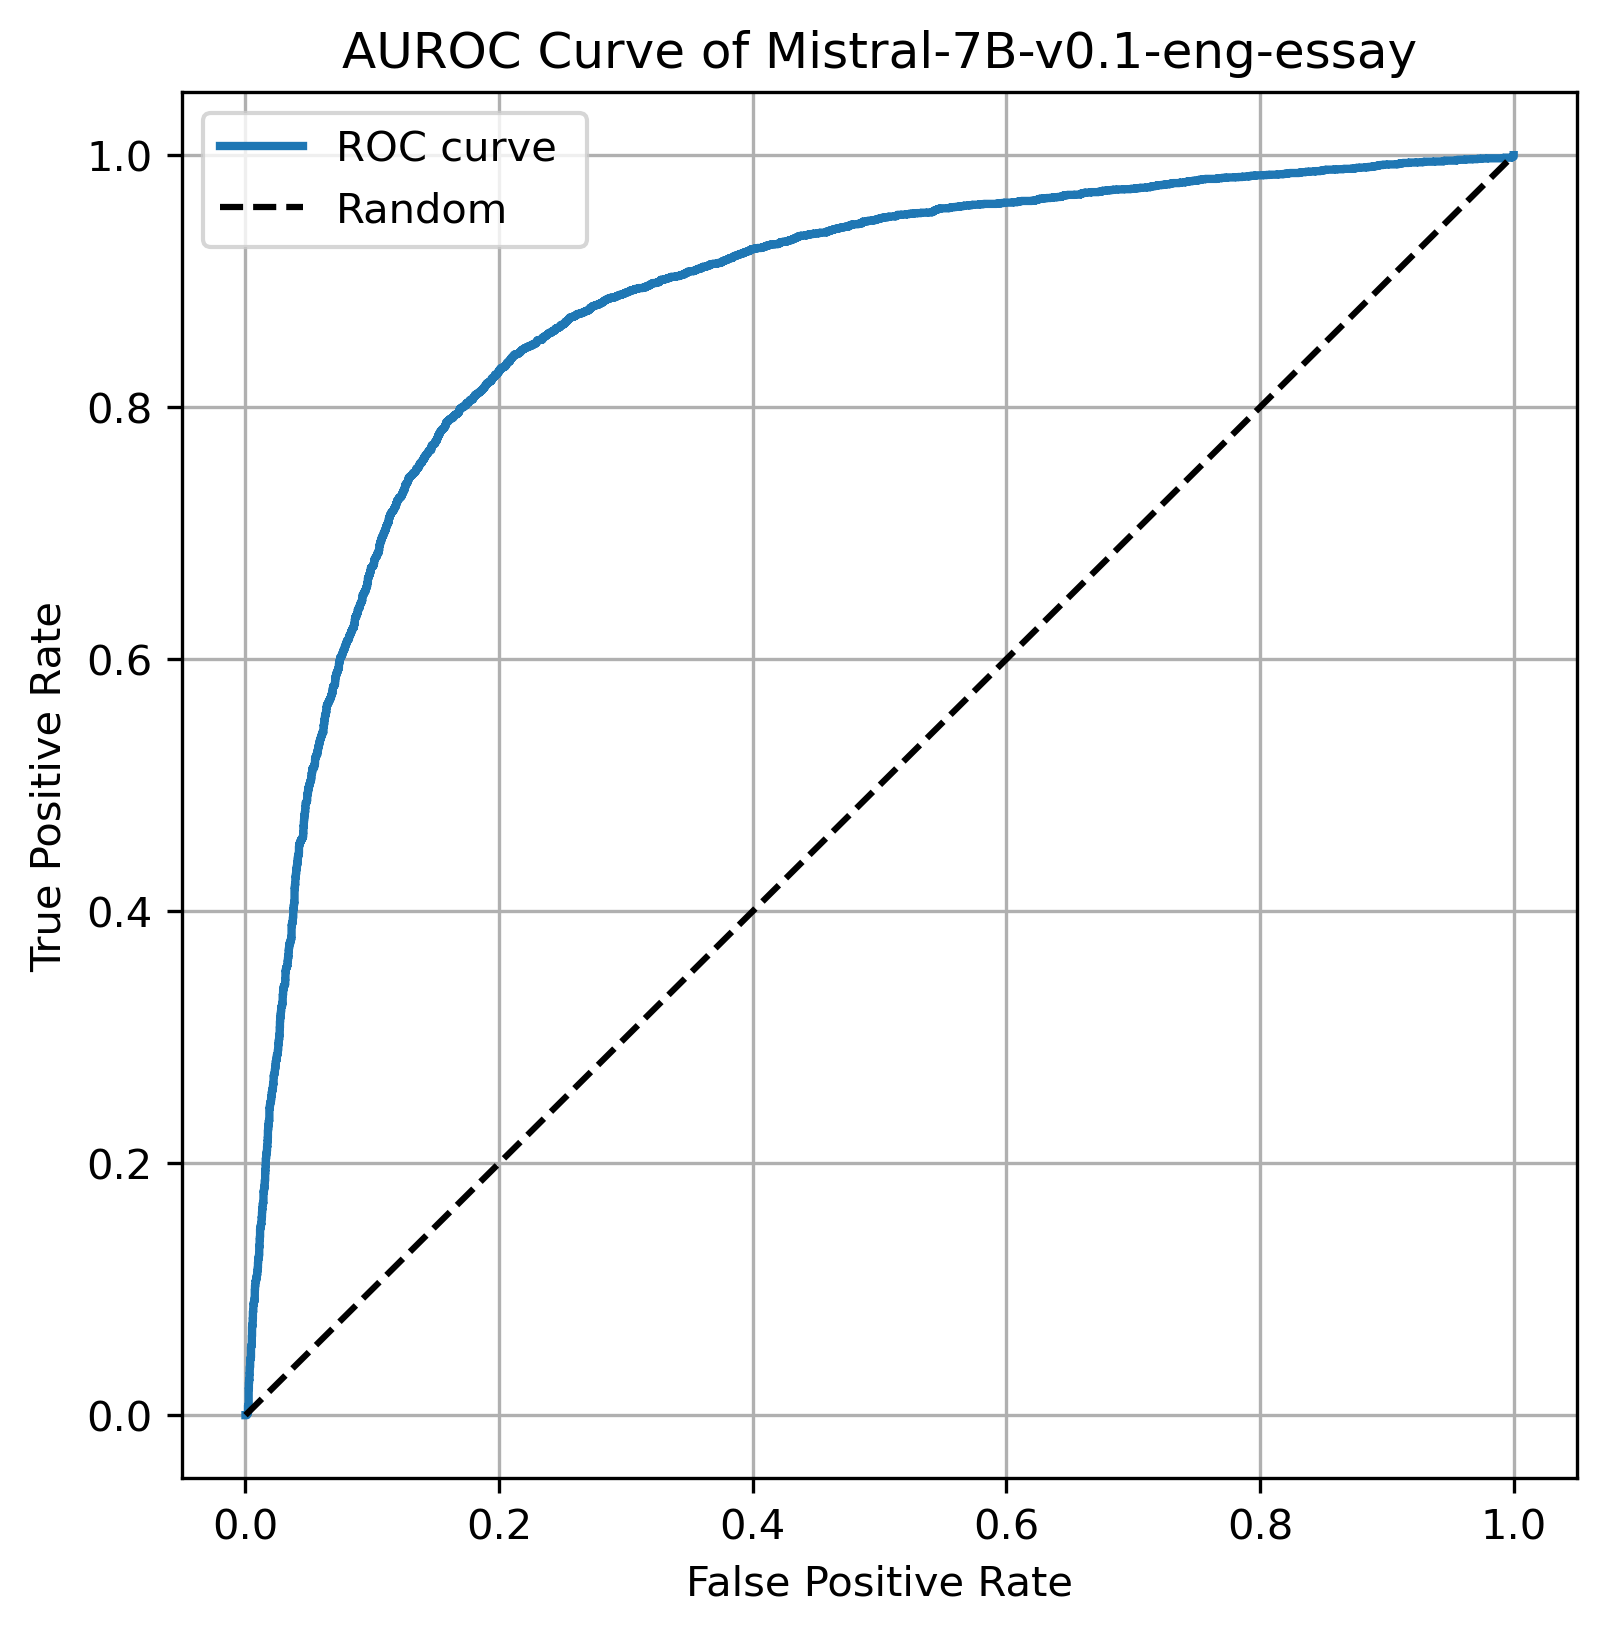
\includegraphics[width=\linewidth]{images/Mistral-7B-v0.1-eng-essay.png}

  \column{0.2\textwidth}
    \centering
    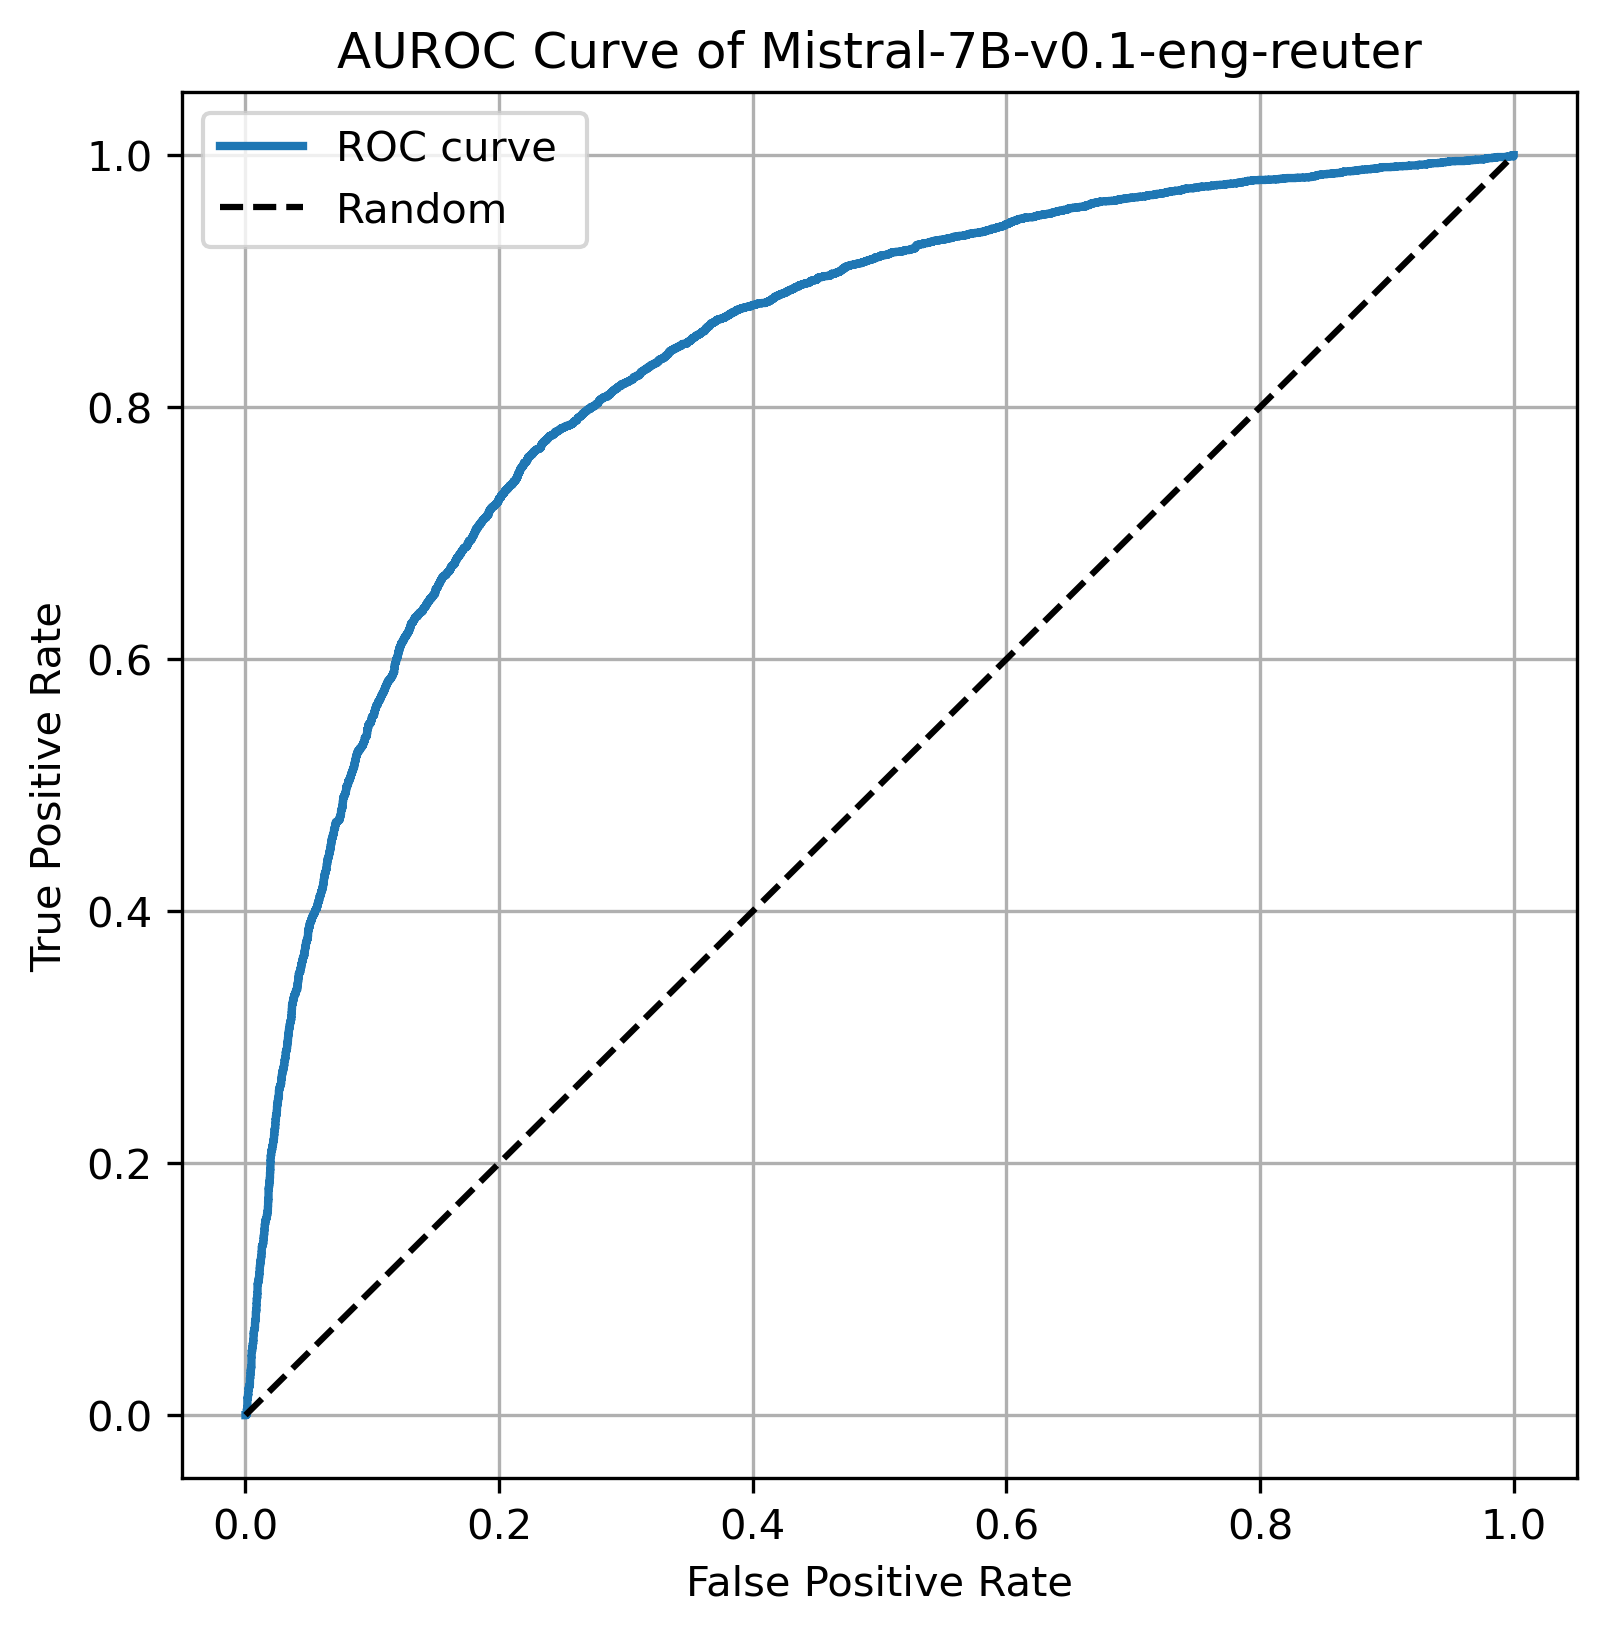
\includegraphics[width=\linewidth]{images/Mistral-7B-v0.1-eng-reuter.png}

  \column{0.2\textwidth}
    \centering
    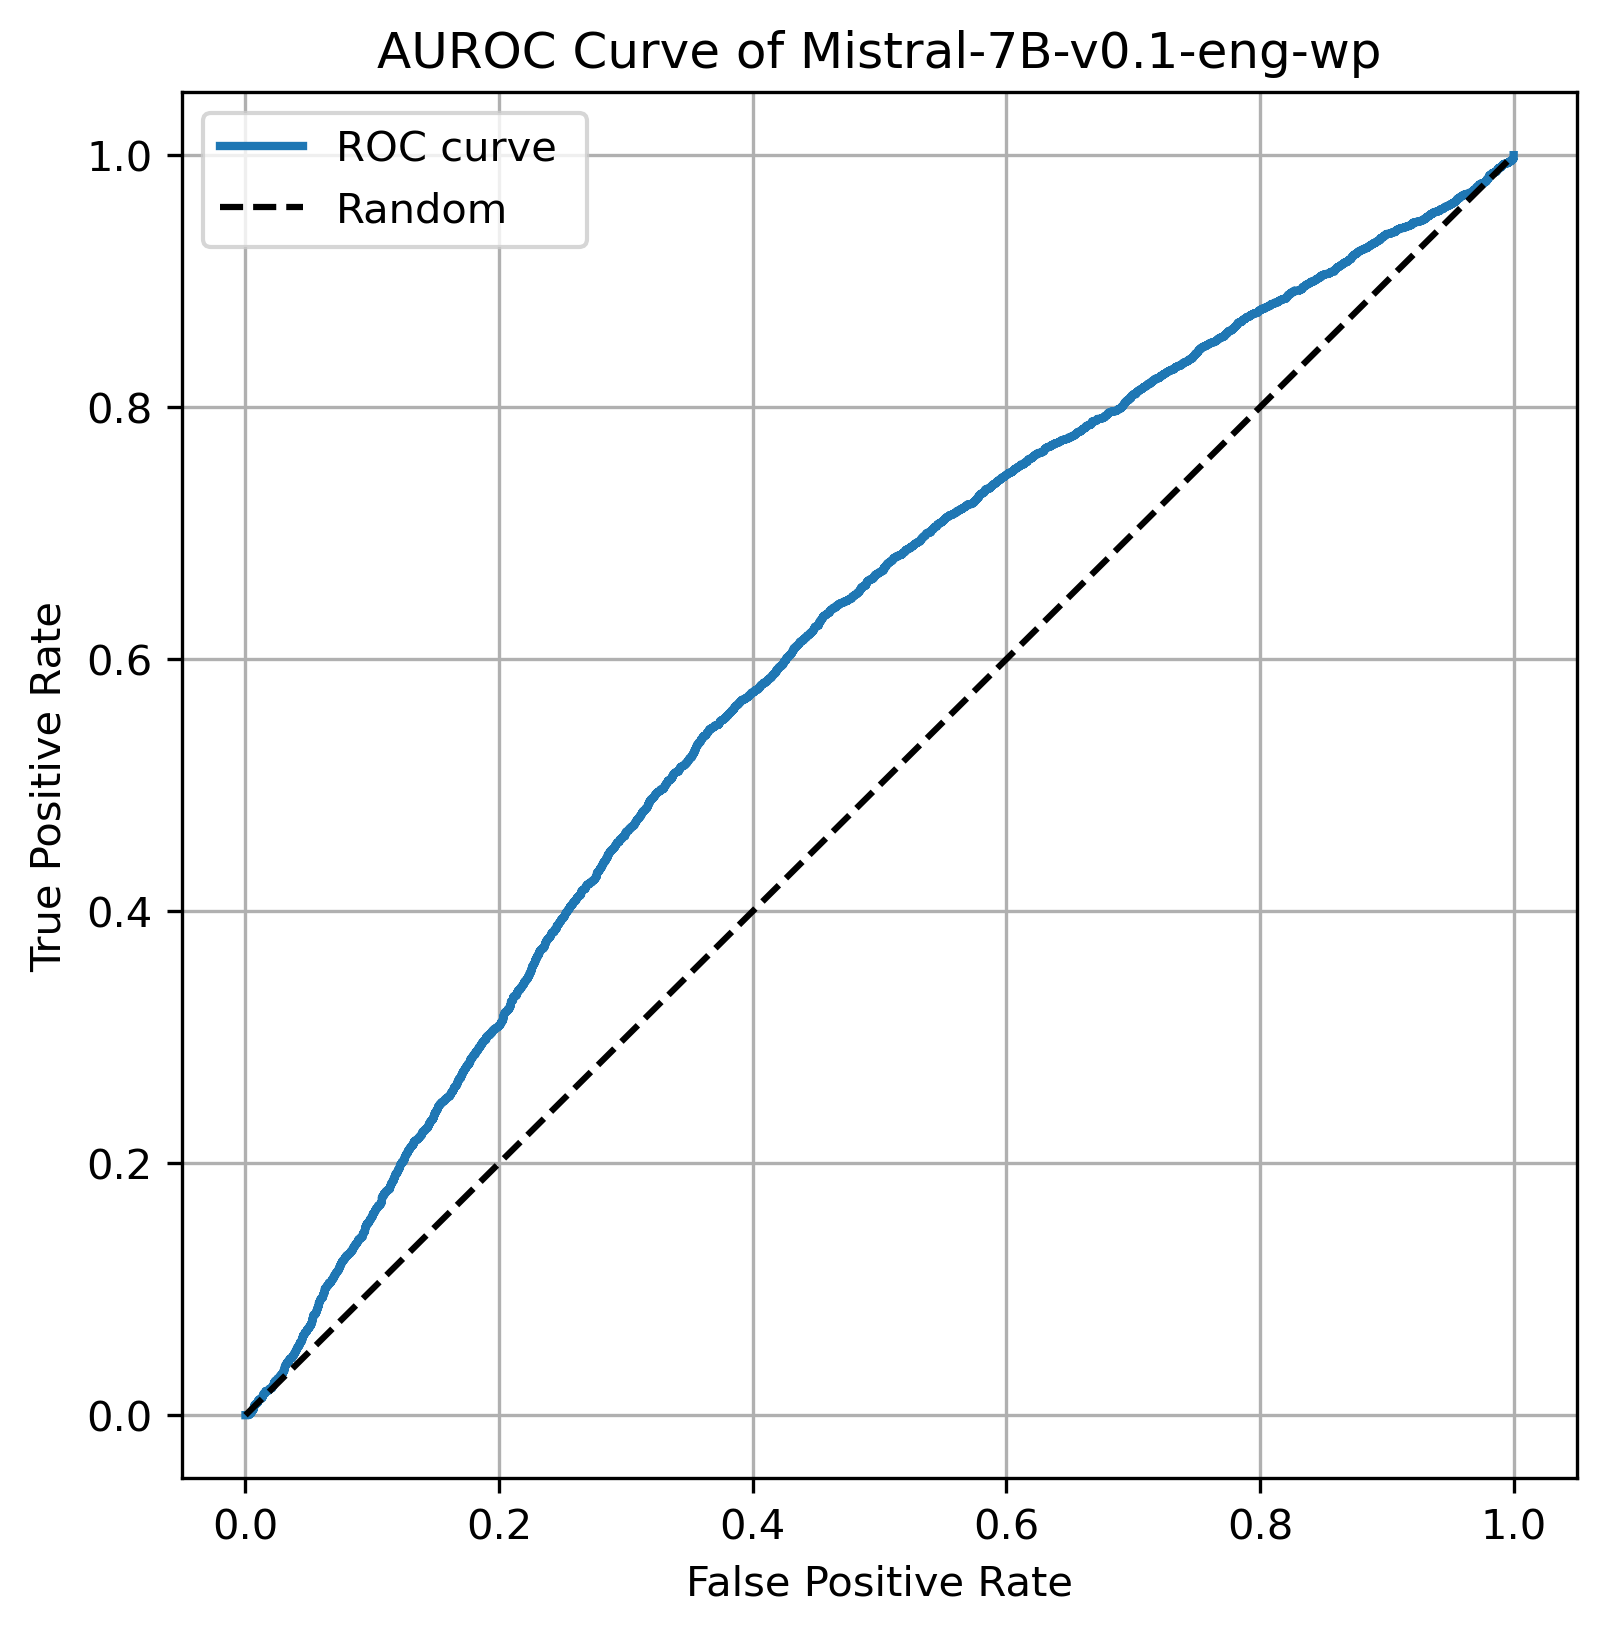
\includegraphics[width=\linewidth]{images/Mistral-7B-v0.1-eng-wp.png}
\end{columns}
\begin{itemize}
  \item On the essay and reuter, the ROC curve of \textbf{Mistral-7B-v0.1} is closer to the top-left corner, indicating stronger ability to \textbf{distinguish positive and negative samples}.
  \item The ROC curves on the\textbf{ wp} are closer to the diagonal line, suggesting a higher chance of random guessing.
\end{itemize}

\end{frame}

\begin{frame}{Zero-shot  Detection:Metrics Comparison (Eng)}
\centering
\tiny
\setlength{\tabcolsep}{2pt}
\renewcommand{\arraystretch}{1.0}
\vspace{0.3cm}
\resizebox{0.7\textwidth}{!}{%
\begin{tabular}{|l|c|c|c|}
\hline
\textbf{FT domain} & \textbf{essay} & \textbf{reuter} & \textbf{wp} \\
\hline
Accuracy & 0.6510 & 0.6795 & 0.6330 \\
\hline
AUROC & 0.6899 & 0.7348 & 0.6732 \\
\hline
\end{tabular}%
}
\vspace{0.1cm}
{\scriptsize \captionof{table}{gpt2-xl-Eng}}

\centering
\tiny
\setlength{\tabcolsep}{2pt}
\renewcommand{\arraystretch}{1.0}
\vspace{0.3cm}
\resizebox{0.7\textwidth}{!}{%
\begin{tabular}{|l|c|c|c|}
\hline
\textbf{FT domain} & \textbf{essay} & \textbf{reuter} & \textbf{wp} \\
\hline
Accuracy & 0.8133 & 0.7675 & 0.5855 \\
\hline
AUROC & 0.8798 & 0.8375 & 0.6044 \\
\hline
\end{tabular}%
}
\vspace{0.1cm}
{\scriptsize \captionof{table}{Mistral-7B-v0.1-Eng}}
\end{frame}

%-------------
\begin{frame}{Zero-shot Detection (Zh)}

\centering
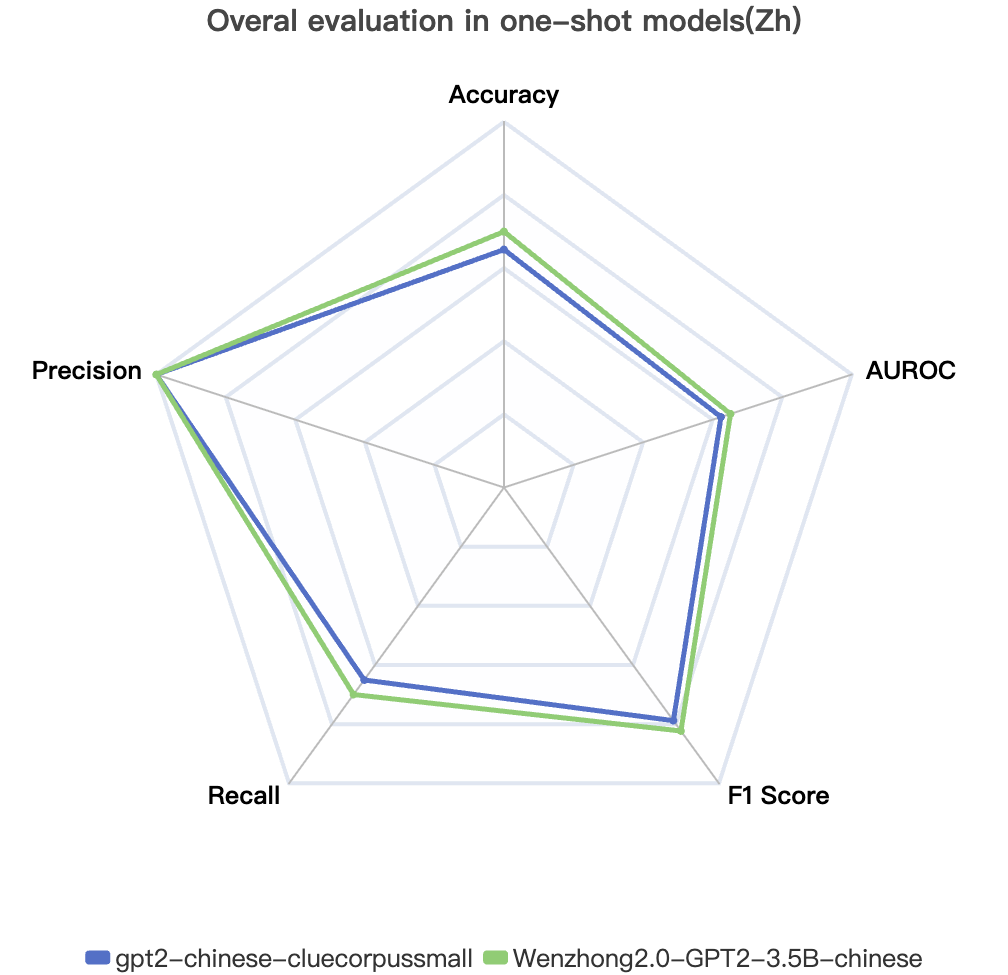
\includegraphics[width=0.5\textwidth]{images/Overal evaluation in one-shot models(Zh).png}

\vspace{-0.2em}
\begin{flushleft}
\scriptsize
\textbf{Wenzhong2.0-GPT2-3.5B-chinese} slightly outperforms gpt2-chinese-cluecorpussmall across most metrics in one-shot detection for Chinese texts.
\normalize
\end{flushleft}

\end{frame}
%--------------
\begin{frame}{Zero-shot Detection:Accuracy (Zh)}
    \begin{figure}
        \centering
        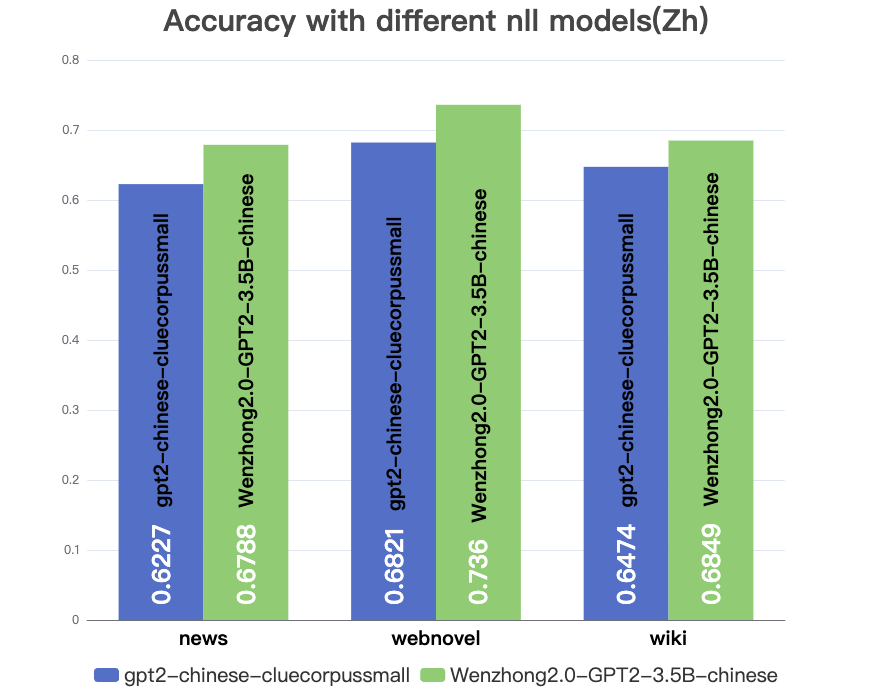
\includegraphics[width=0.5\linewidth]{images/Accuracy with different nll models(Zh).png}
        \label{fig:enter-label}
    \end{figure}
    \begin{itemize}
    \item \textbf{Wenzhong2.0-GPT2-3.5B} outperforms gpt2-chinese-cluecorpussmall across all domains
    \item Both models achieve the highest accuracy and AUROC in the \textbf{webnovel} domain(\textbf{0.73 and 0.82})
    \item Detecting differences in \textbf{news} texts is more challenging(\textbf{0.64 and 0.68})
\end{itemize}
\end{frame}

\begin{frame}{Zero-shot Detection:AUROC curve (Zh)}
\begin{columns}[t]
  \column{0.2\textwidth}
    \centering
    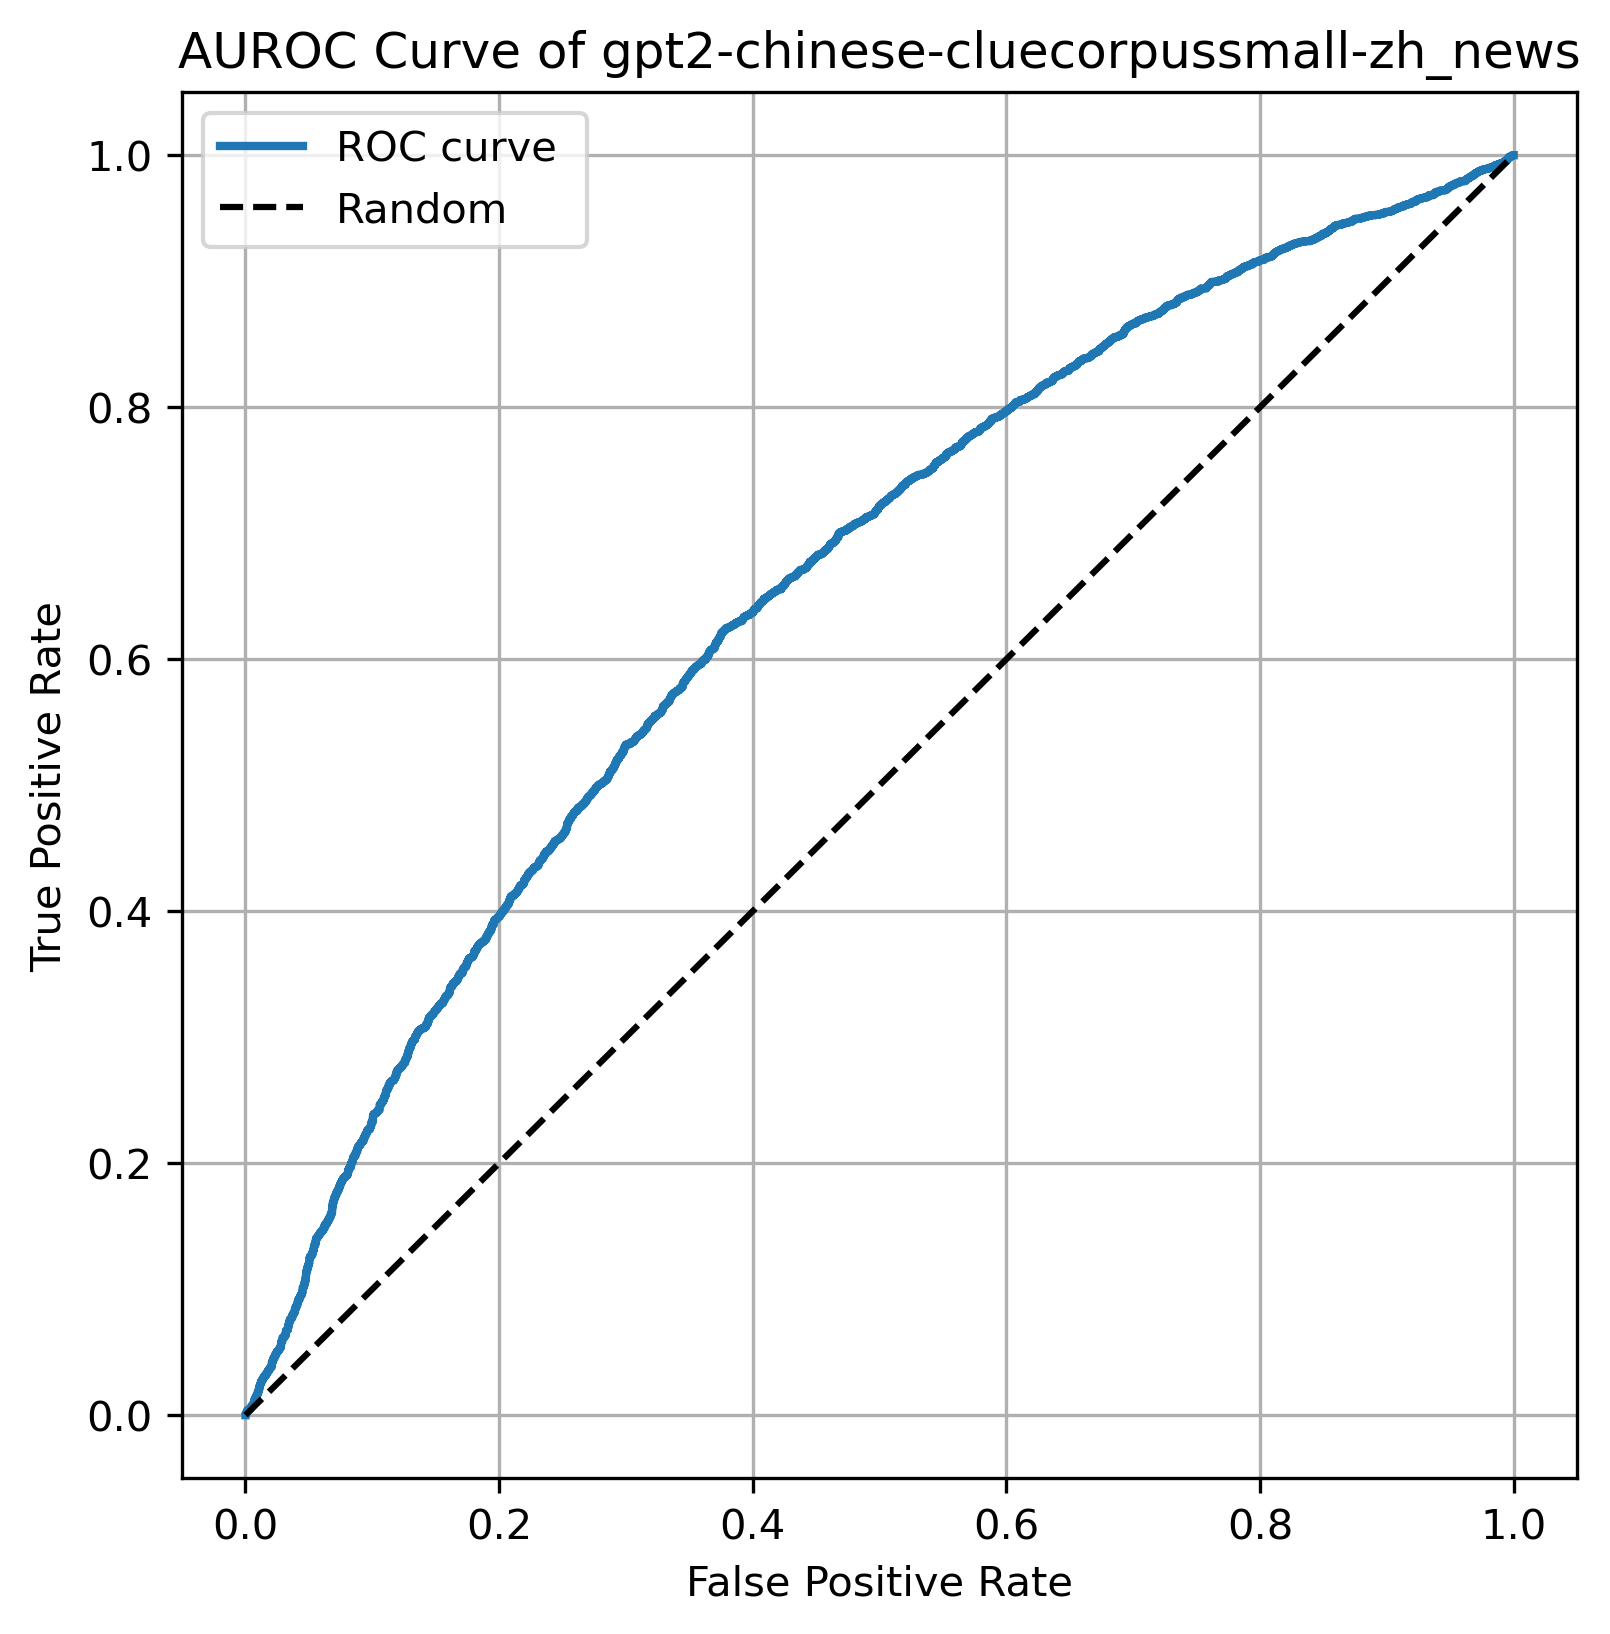
\includegraphics[width=\linewidth]{images/gpt2-chinese-cluecorpussmall-zh_news.png}

  \column{0.2\textwidth}
    \centering
    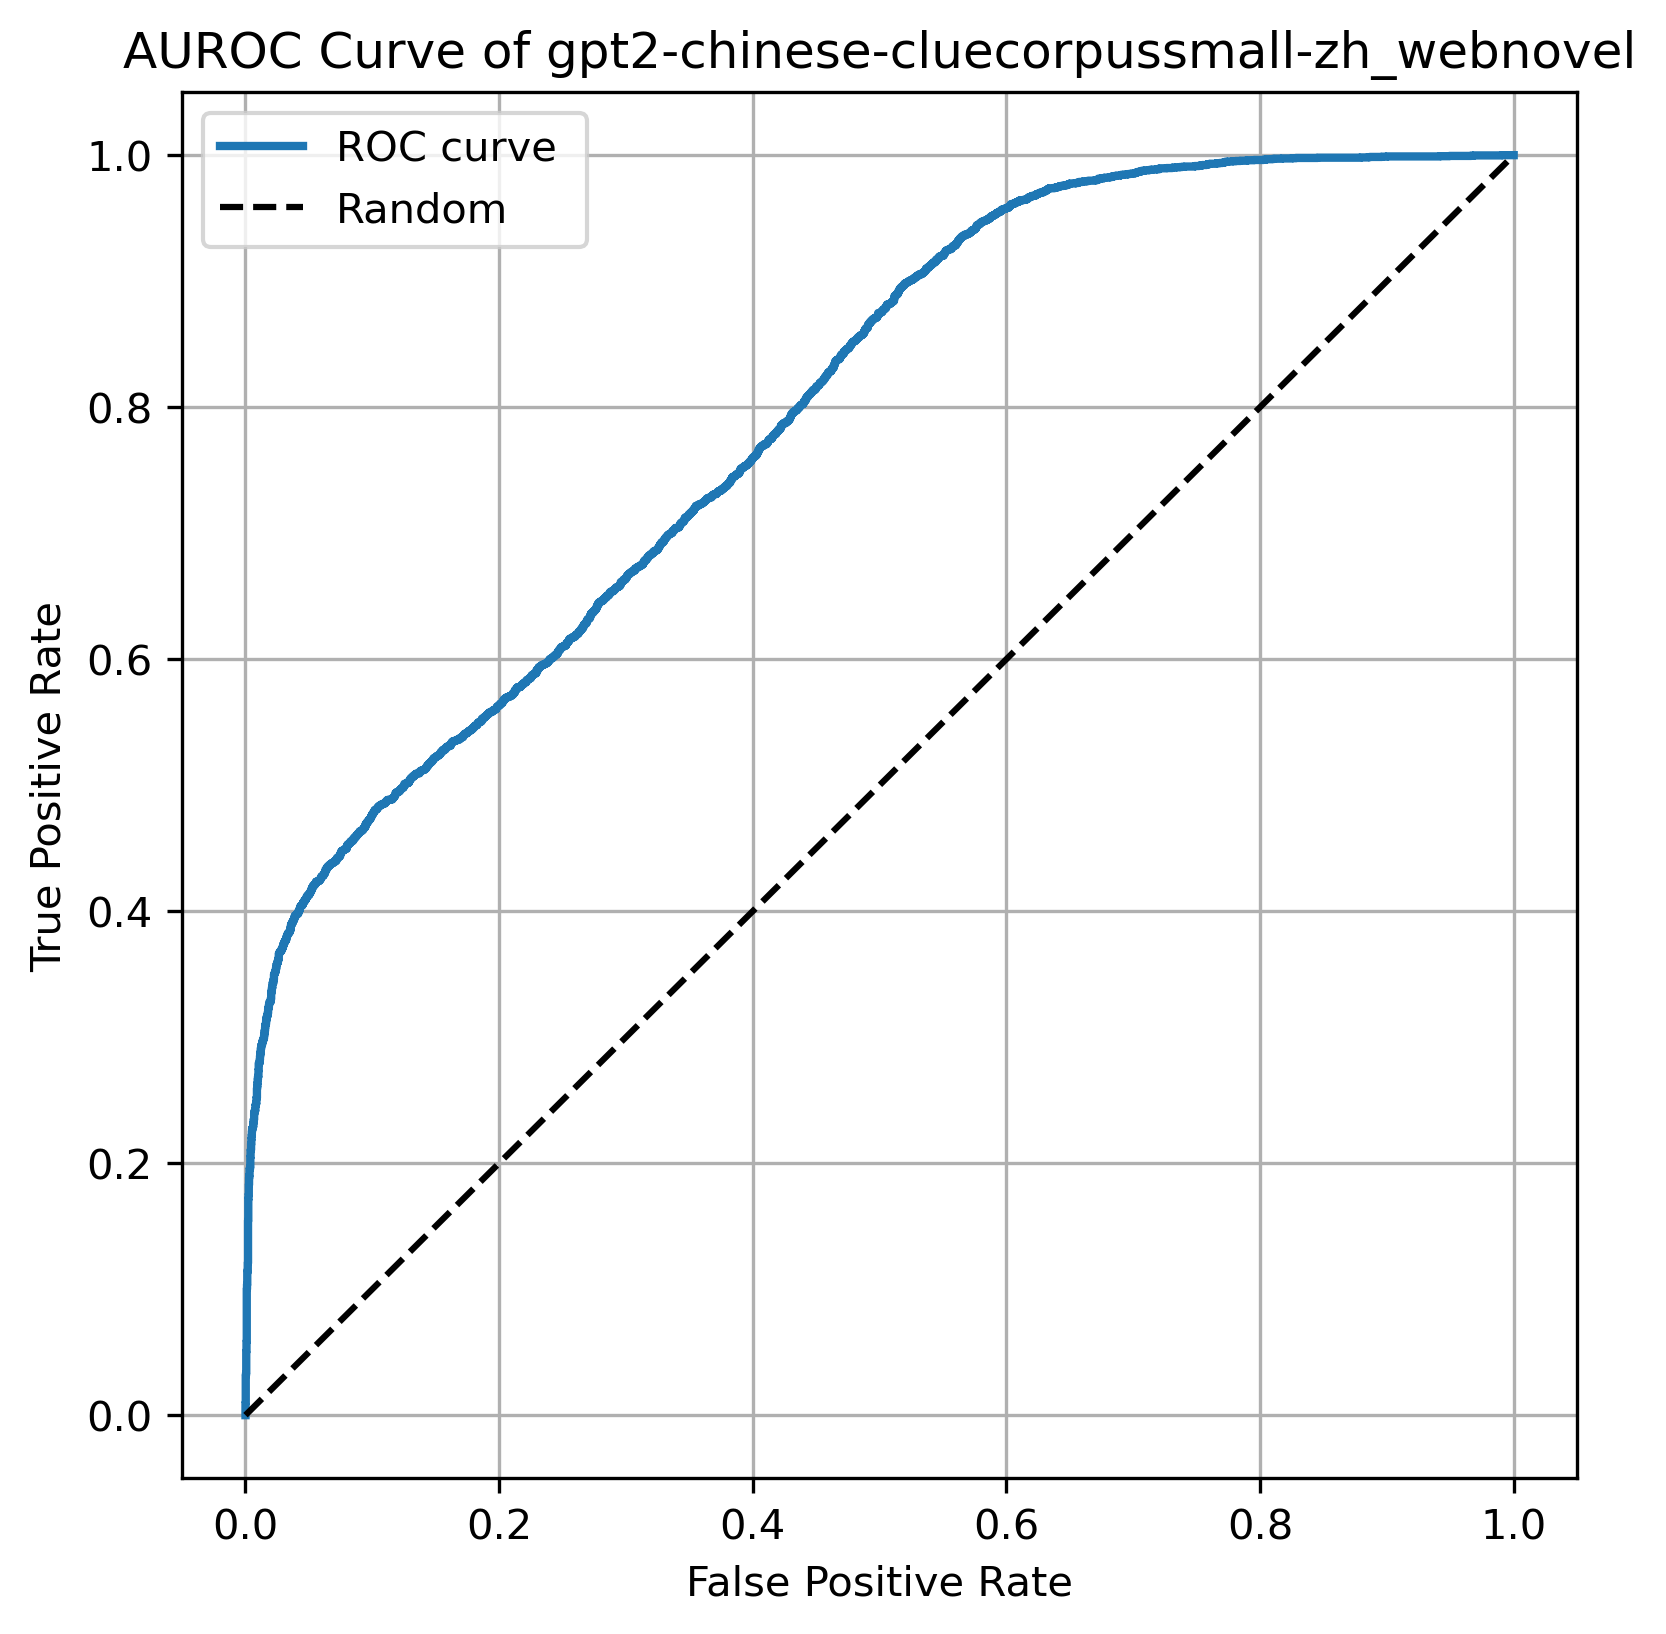
\includegraphics[width=\linewidth]{images/gpt2-chinese-cluecorpussmall-zh_webnovel.png}

  \column{0.2\textwidth}
    \centering
    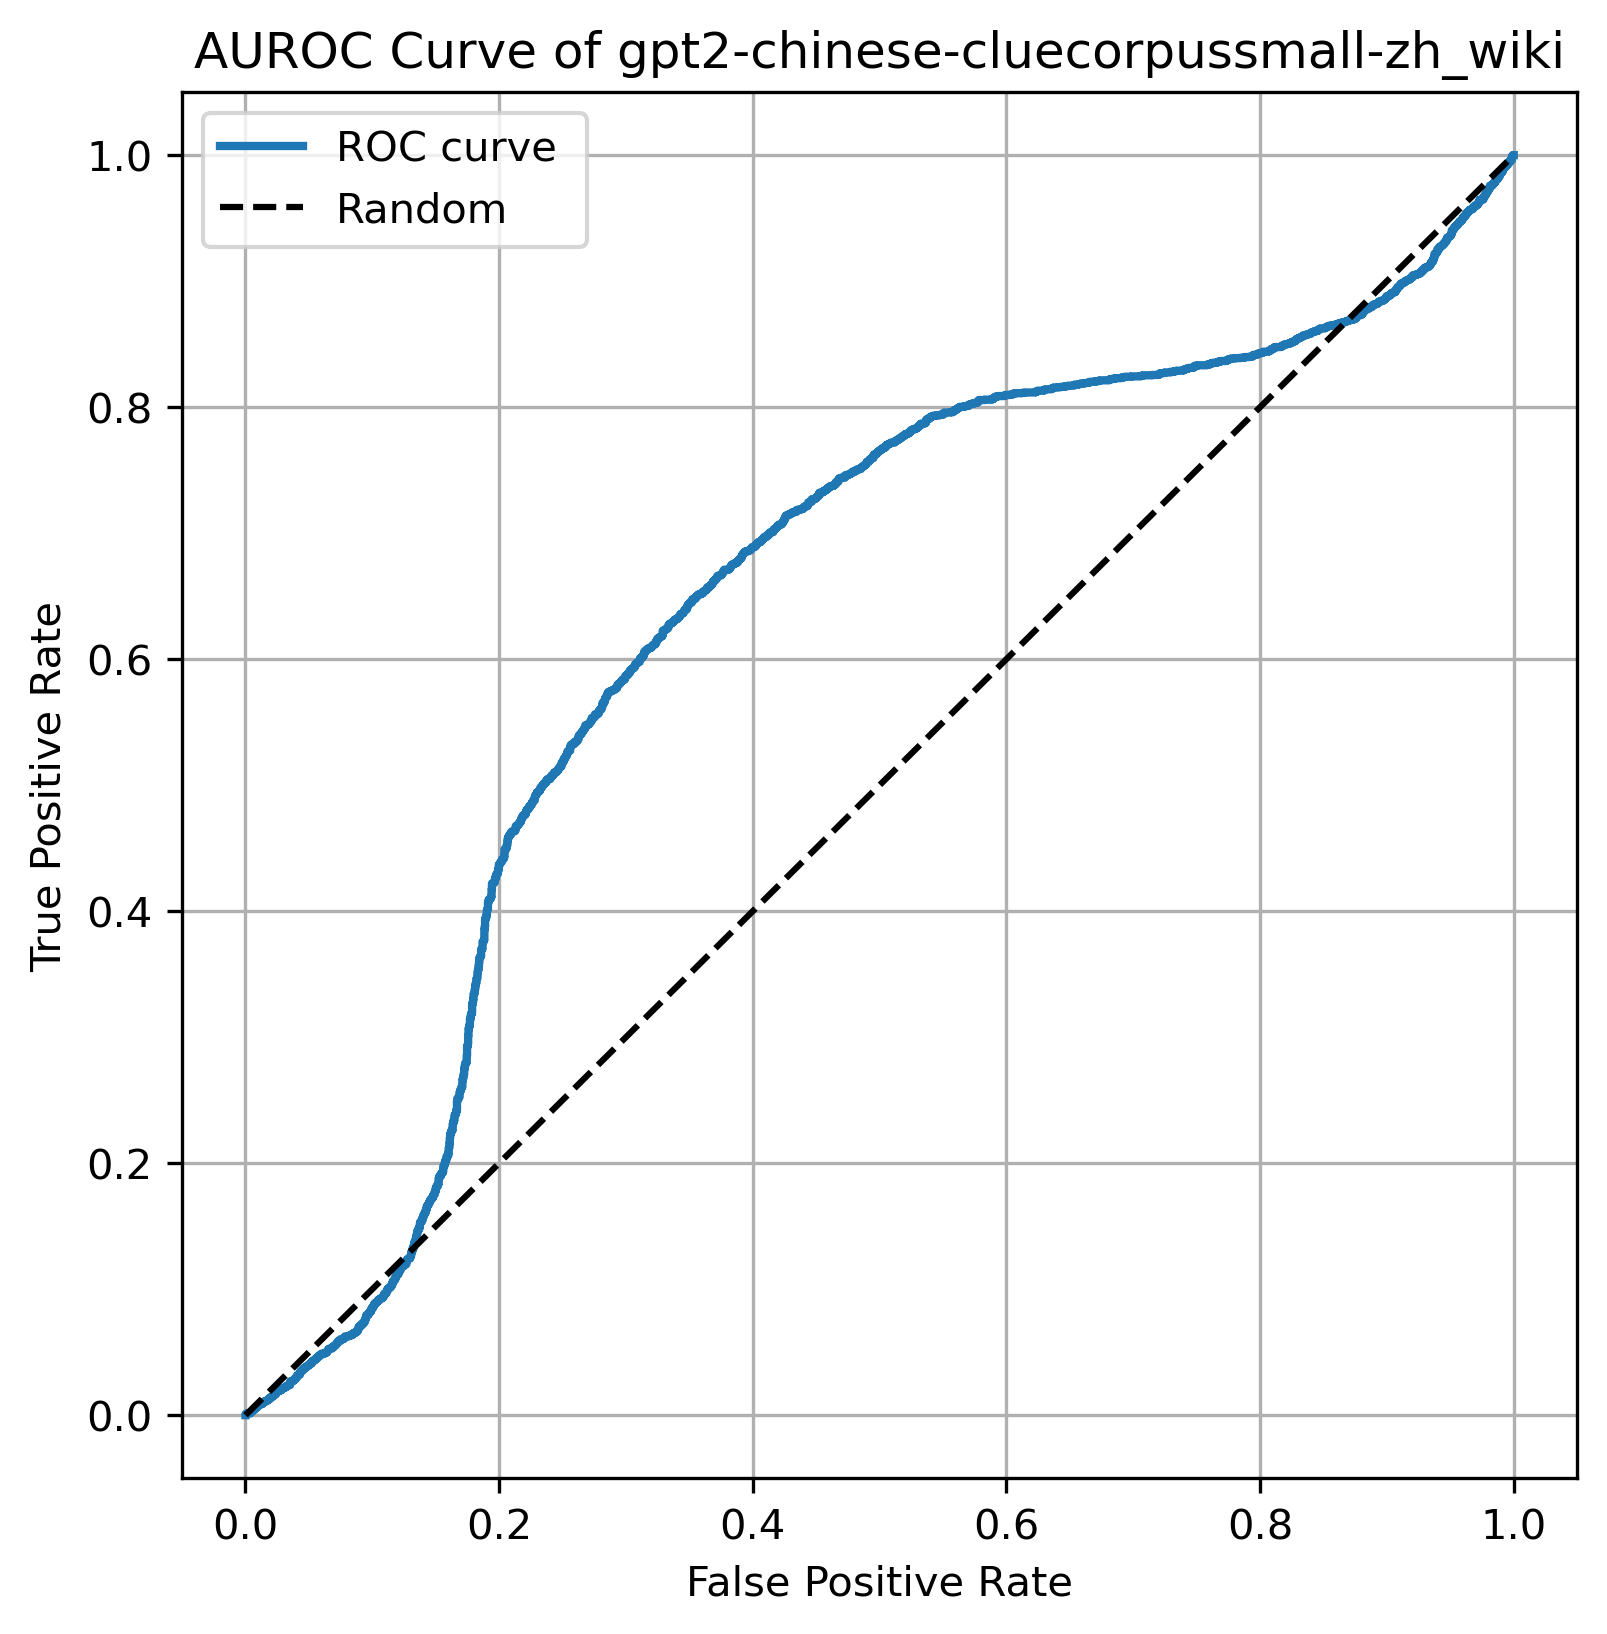
\includegraphics[width=\linewidth]{images/gpt2-chinese-cluecorpussmall-zh_wiki.png}
\end{columns}
\vspace{0.3cm}
\begin{columns}[t]
  \column{0.2\textwidth}
    \centering
    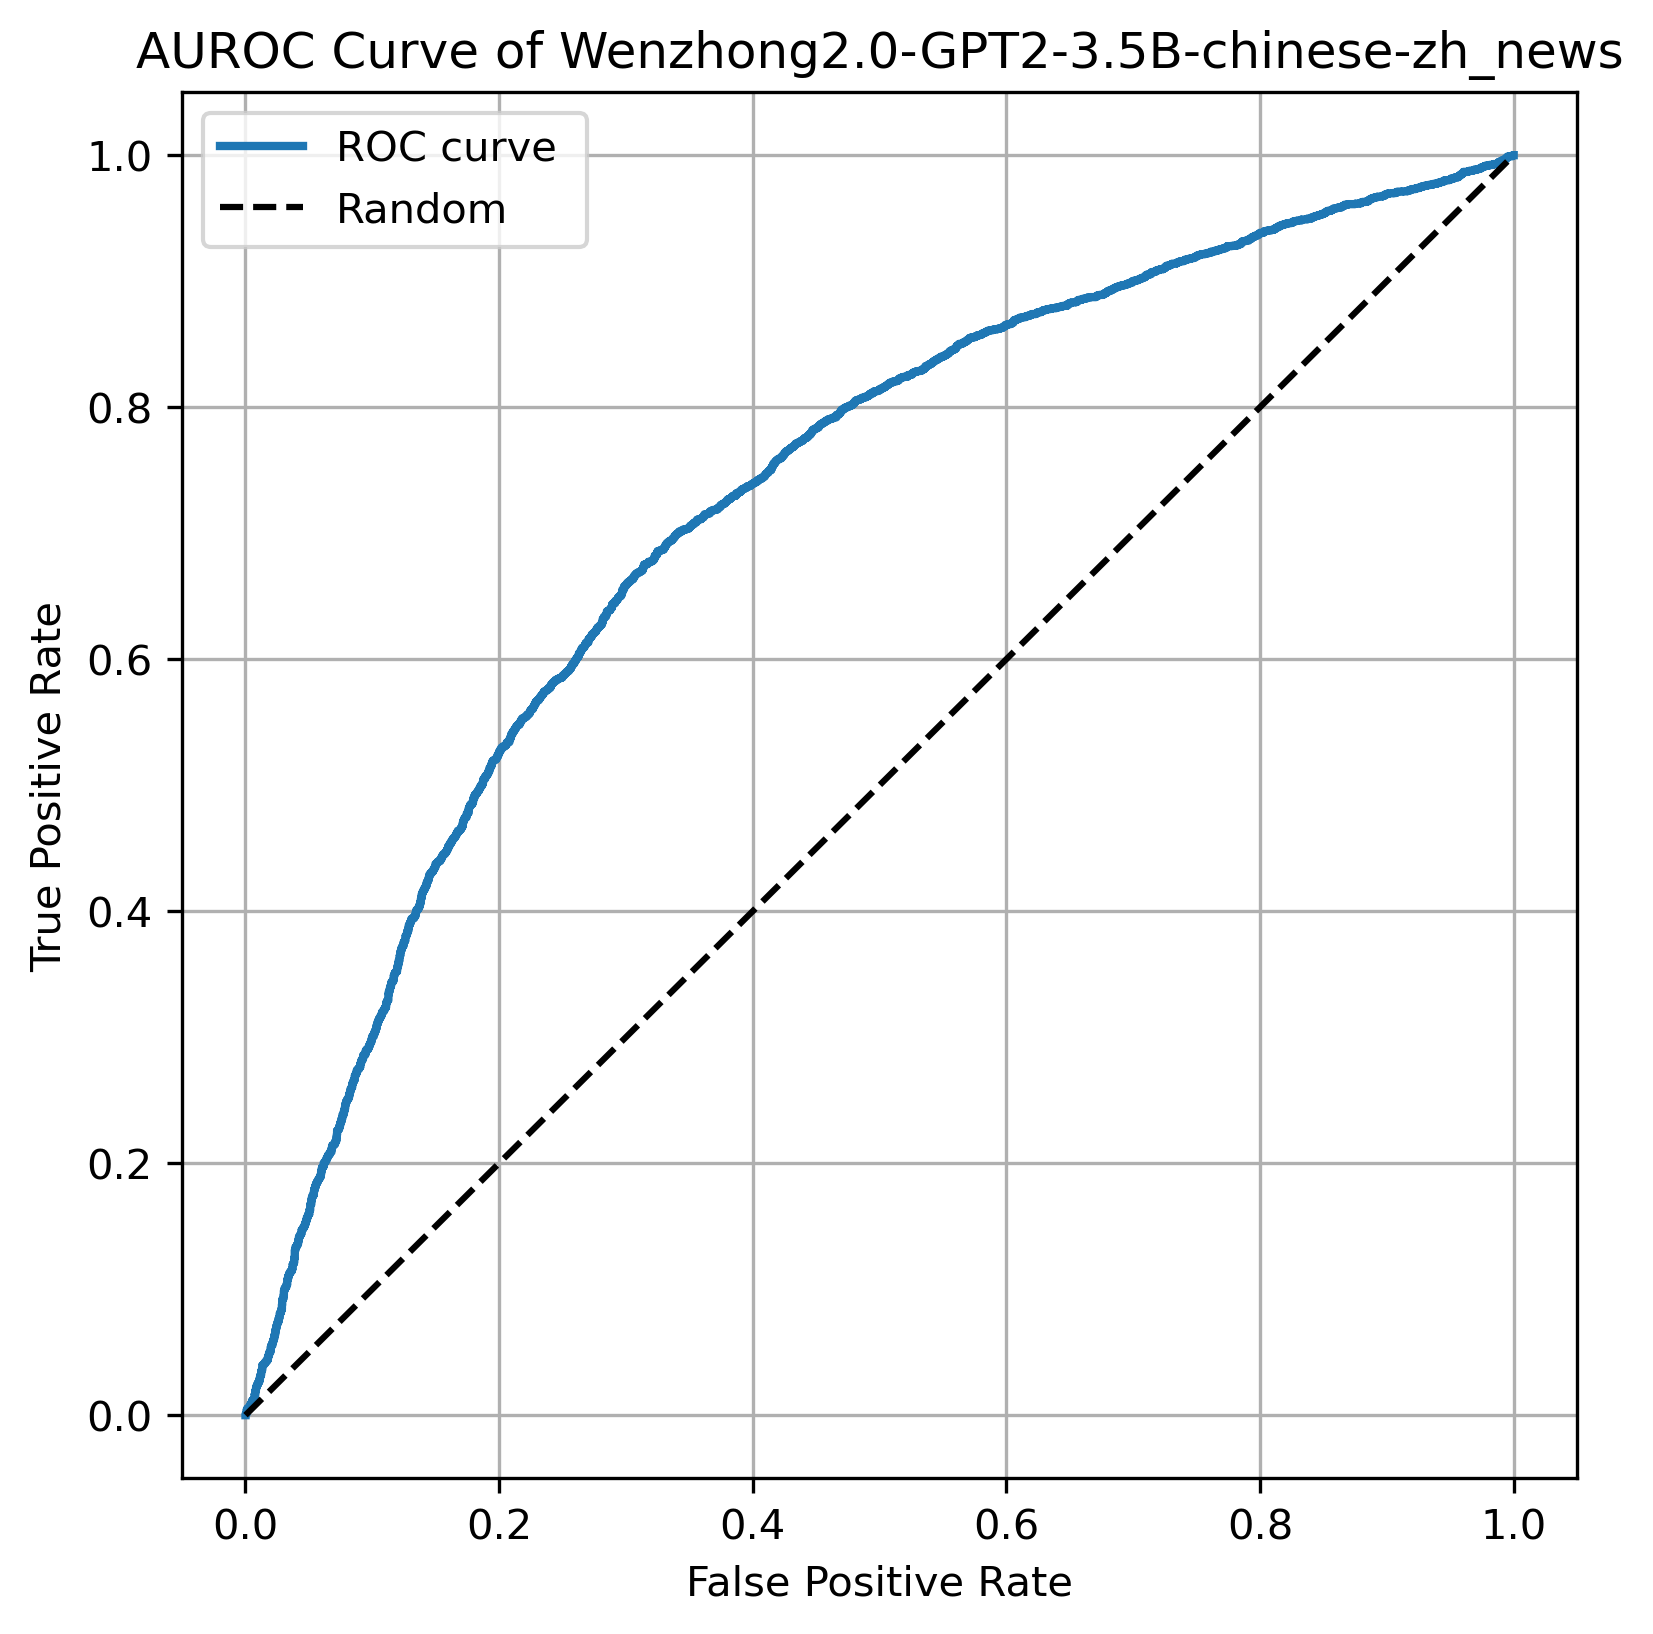
\includegraphics[width=\linewidth]{images/Wenzhong2.0-GPT2-3.5B-chinese-zh_news.png}

  \column{0.2\textwidth}
    \centering
    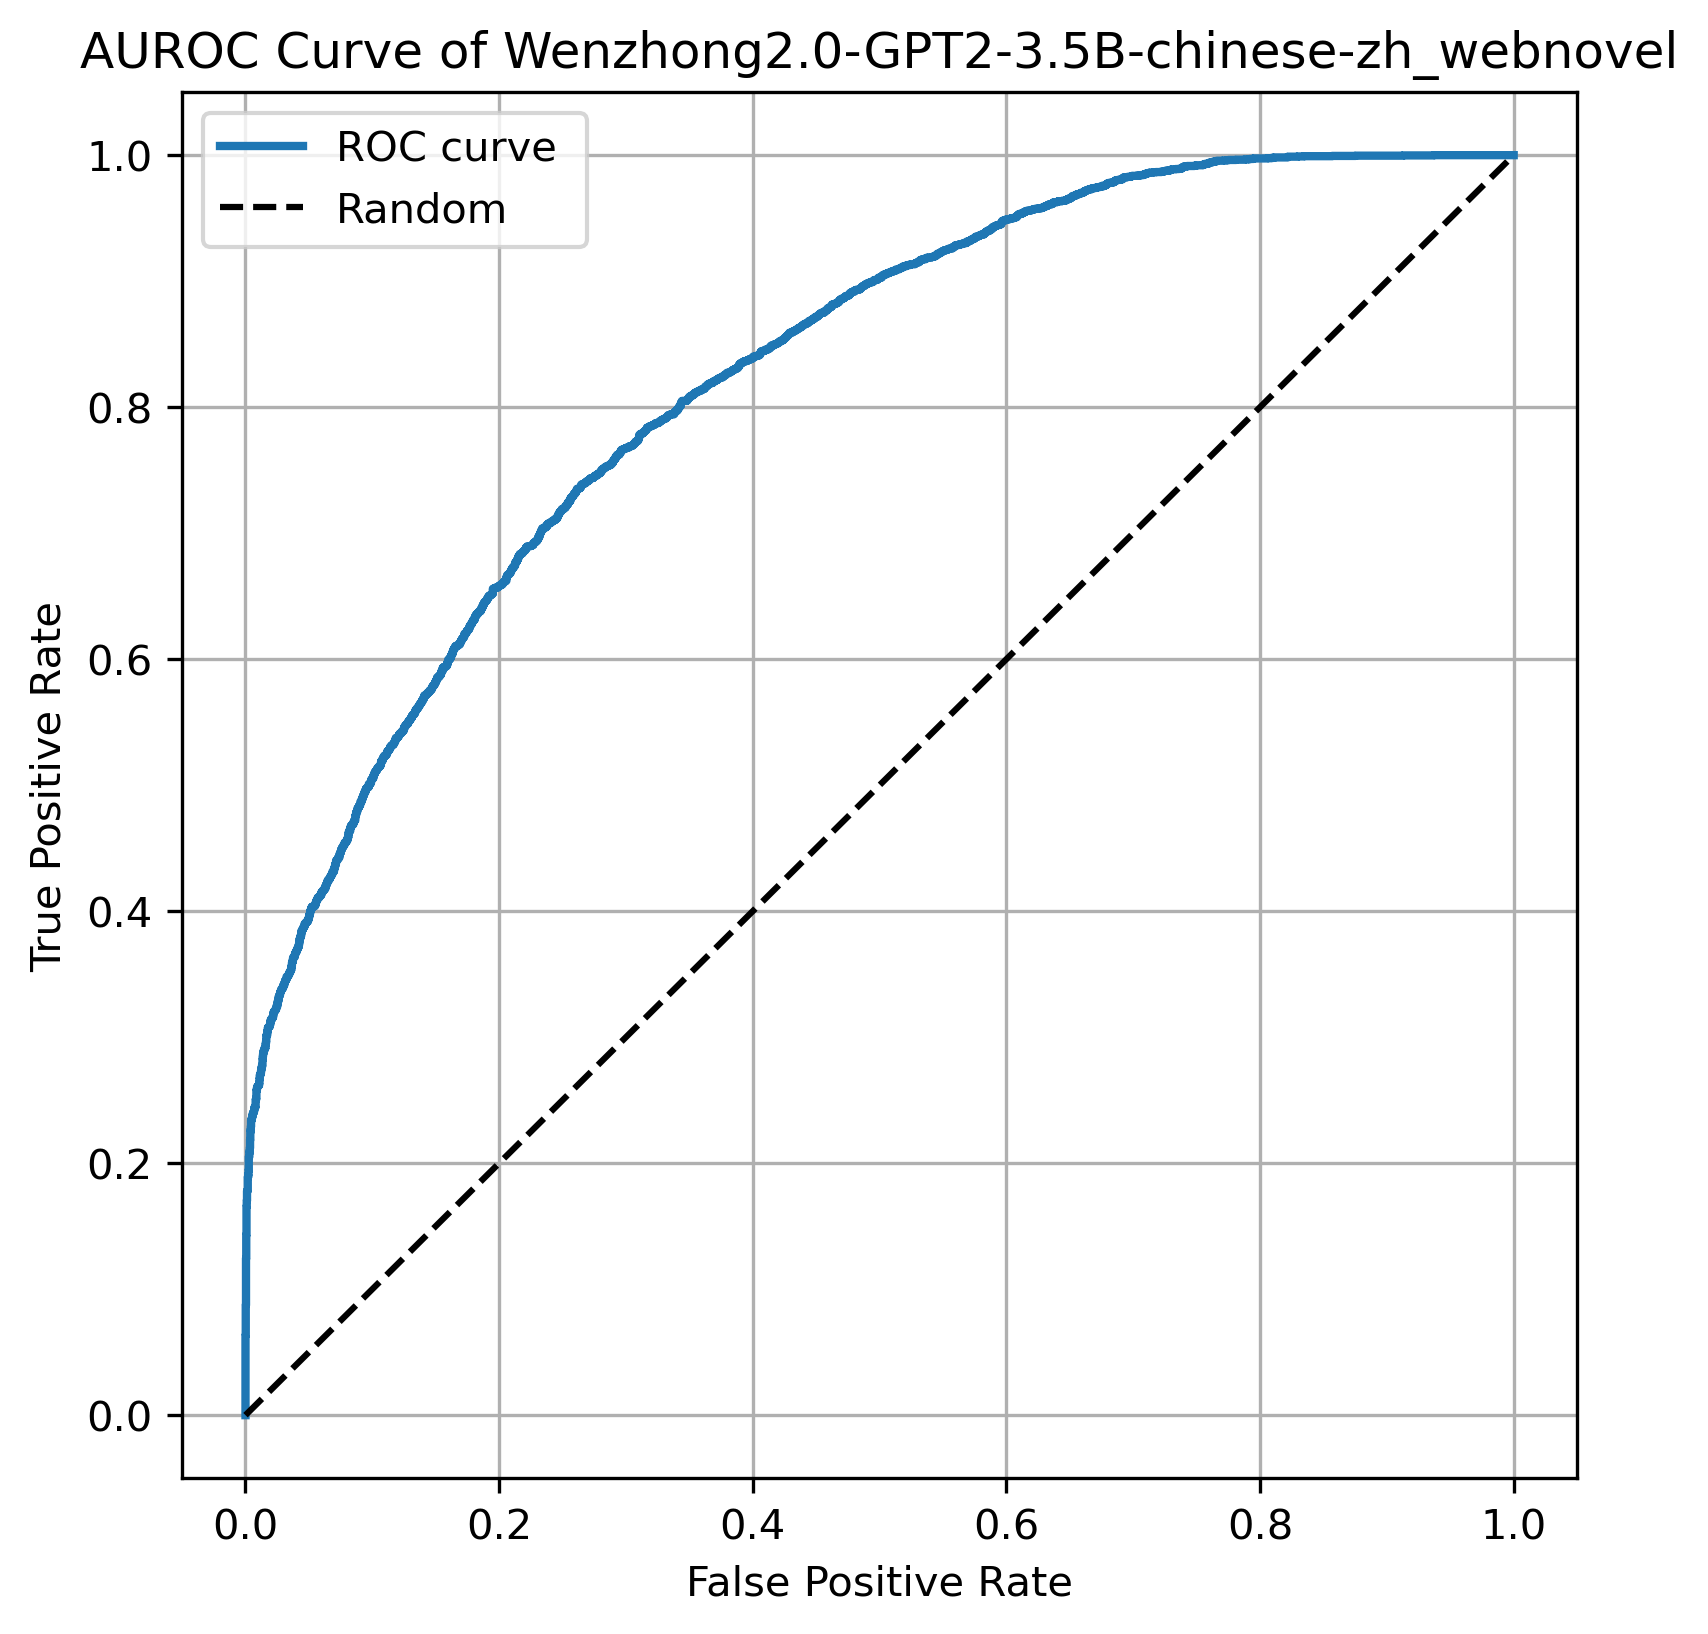
\includegraphics[width=\linewidth]{images/Wenzhong2.0-GPT2-3.5B-chinese-zh_webnovel.png}

  \column{0.2\textwidth}
    \centering
    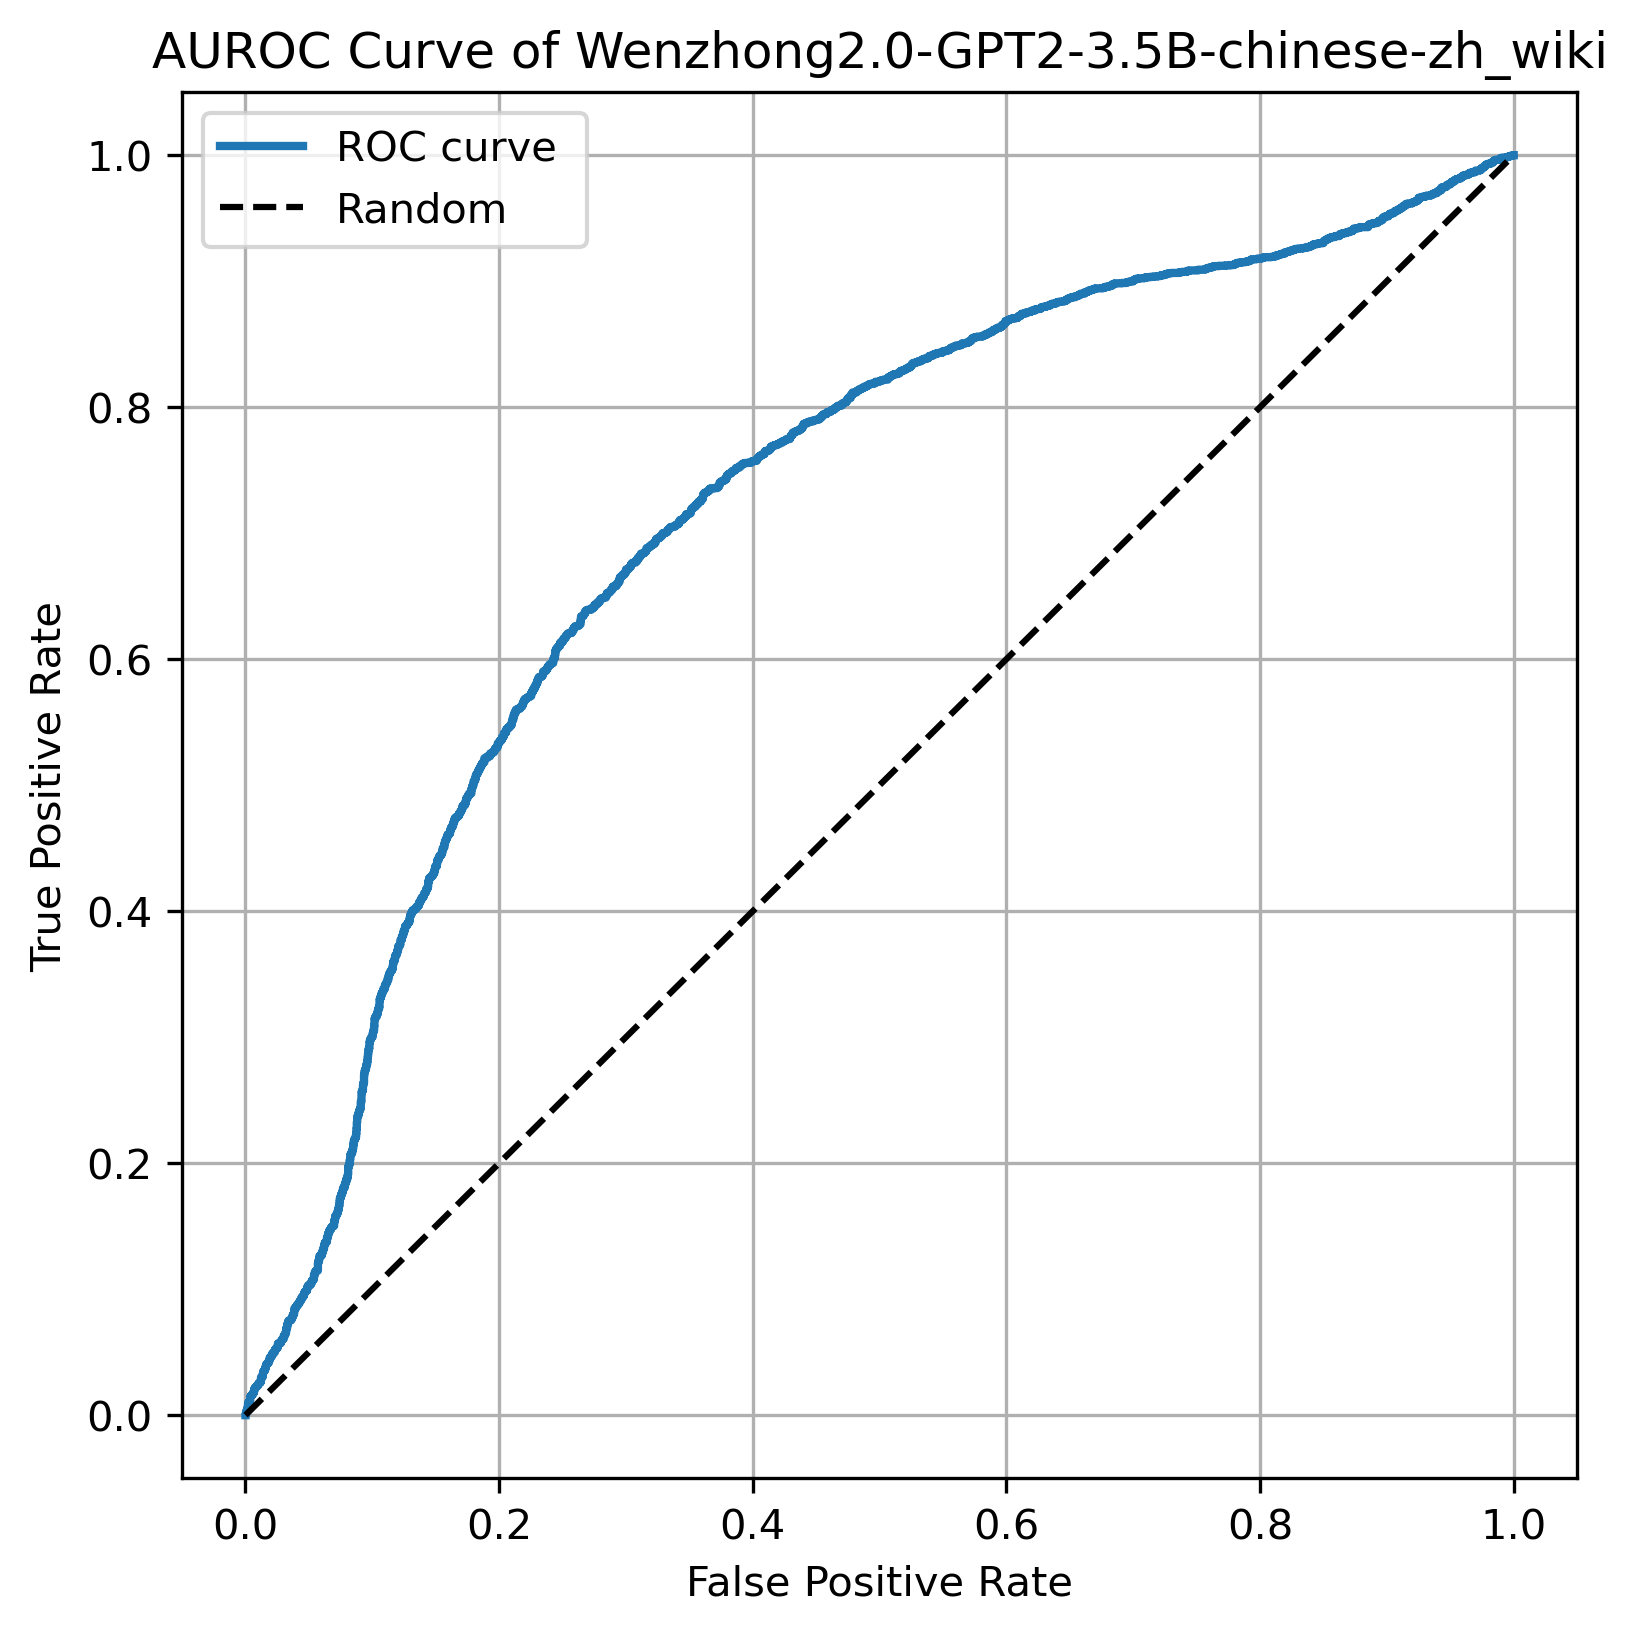
\includegraphics[width=\linewidth]{images/Wenzhong2.0-GPT2-3.5B-chinese-zh_wiki.png}
\end{columns}
\begin{itemize}
  \item The ROC curves for g\textbf{pt2-chinese-cluecorpussmall} show good \textbf{early rise} in news and webnovel datasets but remain flat and close to the diagonal in the wiki dataset, indicating weaker discrimination.
  \item The \textbf{Wenzhong2.0-GPT2-3.5B} has steeper, more left-top concentrated curves in news and webnovel datasets, demonstrating stronger classification performance.
\end{itemize}
\end{frame}

\begin{frame}{Zero-shot  Detection:Metrics Comparison (Zh)}
\centering
\tiny
\setlength{\tabcolsep}{2pt}
\renewcommand{\arraystretch}{1.0}
\vspace{0.3cm}
\resizebox{0.7\textwidth}{!}{%
\begin{tabular}{|l|c|c|c|}
\hline
\textbf{FT domain} & \textbf{news} & \textbf{webnovel} & \textbf{wiki} \\
\hline
Accuracy & 0.6227 & 0.6821 & 0.6474 \\
\hline
AUROC & 0.6561 & 0.7933 & 0.6381 \\
\hline
\end{tabular}%
}
\vspace{0.1cm}
{\scriptsize \captionof{table}{gpt2-chinese-cluecorpussmall-Zh}}

\centering
\tiny
\setlength{\tabcolsep}{2pt}
\renewcommand{\arraystretch}{1.0}
\vspace{0.3cm}
\resizebox{0.7\textwidth}{!}{%
\begin{tabular}{|l|c|c|c|}
\hline
\textbf{FT domain} & \textbf{news} & \textbf{webnovel} & \textbf{wiki} \\
\hline
Accuracy & 0.6788 & 0.7360 & 0.6849 \\
\hline
AUROC & 0.7232 & 0.8240 & 0.7216 \\
\hline
\end{tabular}%
}
\vspace{0.1cm}
{\scriptsize \captionof{table}{Wenzhong2.0-GPT2-3.5B-chinese-Zh}}
\end{frame}


\section{Result analysis}
\begin{frame}{Method comparison(English in domain)}
\begin{figure}
    \centering
    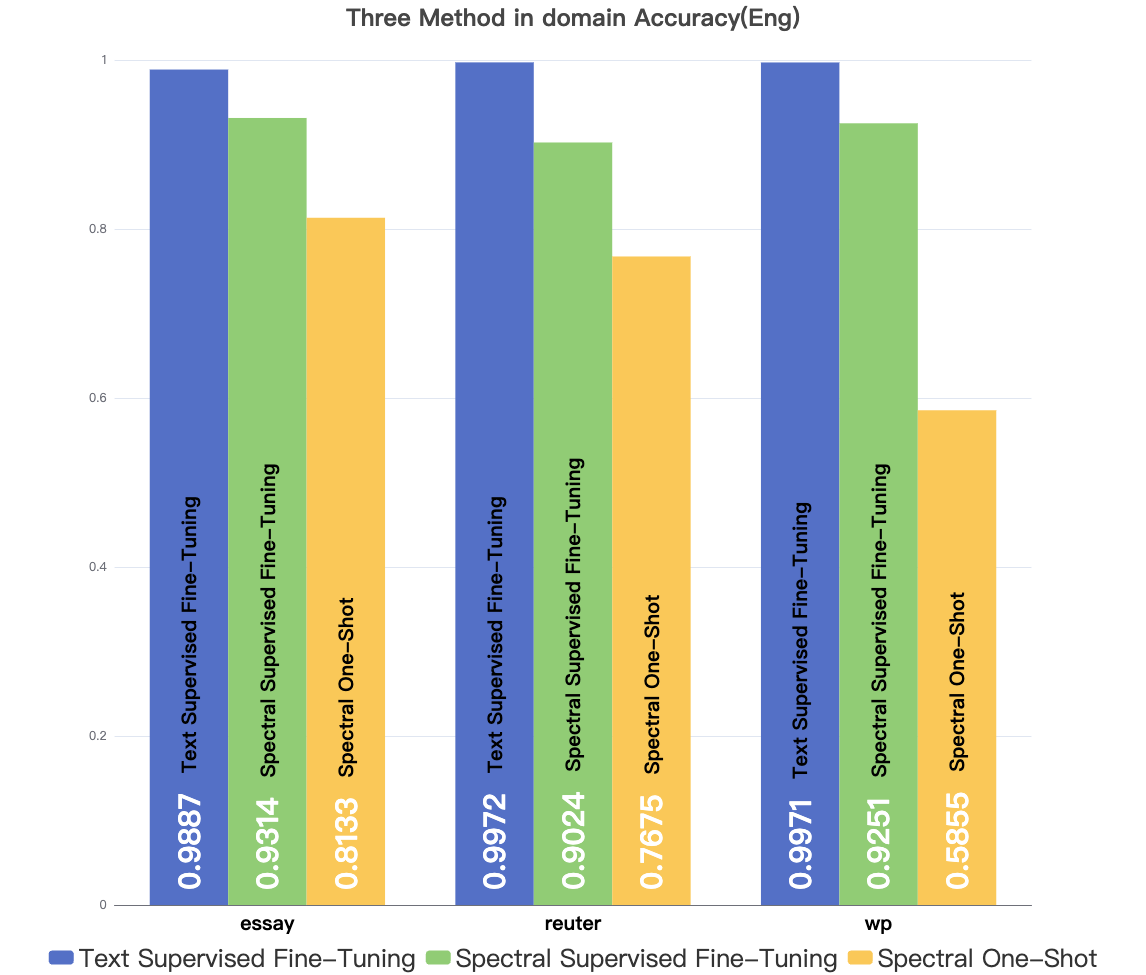
\includegraphics[width=0.5\linewidth]{images/Three Method in domain Accuracy(Eng).png}
\end{figure}
\small{
\begin{item}
    \item \textbf{Text Supervised Fine-Tuning achieves the highest accuracy across all domains}.
    
    \item  \textbf{Zero-Shot} shows the lowest accuracy and \textbf{high domain sensitivity}, especially in the wp domain(\textbf{0.58}).
\end{item}
}
\end{frame}

\begin{frame}{Method comparison(English out of domain)}
\begin{figure}
    \centering
    \includegraphics[width=0.4\linewidth]{images/Three Method out of domain Accuracy(Eng).png}
\end{figure}

\vspace{-0.5em}
\small{
\begin{item}
     \item \textbf{Text Supervised Fine-Tuning} demonstrates \textbf{strong generalization across domains}(above 0.85)

    \item S\textbf{pectral Supervised Fine-Tuning} performs poorly in cross-domain(below \textbf{0.6})

    \item \textbf{Spectral Zero-Shot} performs well on \textbf{essay(0.81) and reuter(0.77)}
\end{item}
}
\end{frame}

\begin{frame}{Method comparison(Zh in domain)}
\begin{figure}
    \centering
    \includegraphics[width=0.5\linewidth]{images/Three Method in domain Accuracy(Zh).png}
\end{figure}
\vspace{-0.5em}
\small{
\begin{item}
     \item \textbf{Text Supervised Fine-Tuning} outperforms all other methods in the \textbf{webnovel} domain(\textbf{0.788})

    \item \textbf{Two FourierGPT methods} perform competitively in the \textbf{news and wiki} domains(around \textbf{0.68})
\end{item}
}
\end{frame}

\begin{frame}{Method comparison(Zh out of domain)}
\begin{figure}
    \centering
    \includegraphics[width=0.5\linewidth]{images/Three Method out of domain Accuracy(Zh).png}
\end{figure}
\vspace{-0.5em}
\small{
\begin{item}
    \item Two \textbf{supervised learning} methods performs poorly(below \textbf{0.65})

    \item \textbf{Zero-shot detection} demonstrates \textbf{strong generalization across domains}(above \textbf{0.65})
\end{item}
}
\end{frame}

\begin{frame}{Reasoning}
\small
\begin{enumerate}
    \item \textbf{Which method performs best in in-domain scenarios, and why?}
    
    \textit{Answer:} \\
   Text Supervised \textbf{Fine-Tuning consistently achieves the highest accuracy in in-domain tasks} because it enables the model to learn detailed domain-specific features and patterns, whereas \textbf{Zero-Shot} methods lack access to such labeled examples during training.


    \vspace{0.3cm}
    \item \textbf{Which method performs best in out-of-domain (OOD) scenarios, and why?}
    
    \textit{Answer:} \\
    \textbf{Zero-Shot (One-Shot) methods show better generalization in out-of-domain settings}, especially in the \textbf{Chinese datasets}, because they do not rely heavily on domain-specific training data. Instead, they utilize more generalizable spectral features or pretrained knowledge, making them more adaptable to unseen domains despite lower in-domain accuracy.

    \vspace{0.3cm}
 
\end{enumerate}
\end{frame}
\begin{frame}{Reasoning}
\small
\begin{enumerate}
   \item \textbf{Why do the One-Shot results differ from those reported in essay?}
    
    \textit{Answer:} \\
 Our English dataset is generated by \textbf{gpt3.5-turbo}, which uses \textbf{Reinforcement Learning from Human Feedback (RLHF)} to improve the quality and safety of its generated content by leveraging human feedback. It also undergoes specialized fine-tuning to \textbf{enhance reasoning,  maintain memory and logical consistency} in multi-turn conversations. So it's harder to discriminate it from human than GPT 3.5 which is used in the paper.
    \vspace{0.3cm}
    \item \textbf{Why do supervised methods achieve lower accuracy in Chinese compared to English?}
    
    \textit{Answer:} \\
    The lower accuracy in Chinese supervised learning is mainly due to the increased \textbf{complexity and diversity of the Chinese language}, such as rich characters and more ambiguous context. 
    \end{enumerate}
\end{frame}

\section{Conclusion}


\begin{frame}{Summary}
\begin{itemize}
  \item This project compares \textbf{supervised learning} and \textbf{zero-shot detection} methods for cross-domain text generation detection.
  \item \textbf{Supervised learning} achieves the best performance \textbf{in-domain}, especially with \textbf{text supervised fine-tuning}.
  \item \textbf{Zero-shot detection} demonstrates stronger \textbf{out-of-domain generalization}, particularly on Chinese datasets.
  \item The \textbf{spectrum-based methods} provide effective feature representations to enhance detection robustness.
\end{itemize}
\end{frame}

\begin{frame}{Future Work}
\begin{itemize}
  \item Explore \textbf{more advanced pretrained models}, including larger multilingual models, for detection tasks.
  \item Investigate integrating \textbf{multi-modal information} (e.g., speech, images) to improve detection accuracy.
  \item Develop \textbf{more efficient spectral analysis and feature augmentation techniques} to boost zero-shot detection performance.
  \item Expand datasets in \textbf{size and diversity}, focusing on real-world and varied text sources.
\end{itemize}
\end{frame}
    
\end{document}